\documentclass{CR} % 文本环境

\begin{document}

% 封面
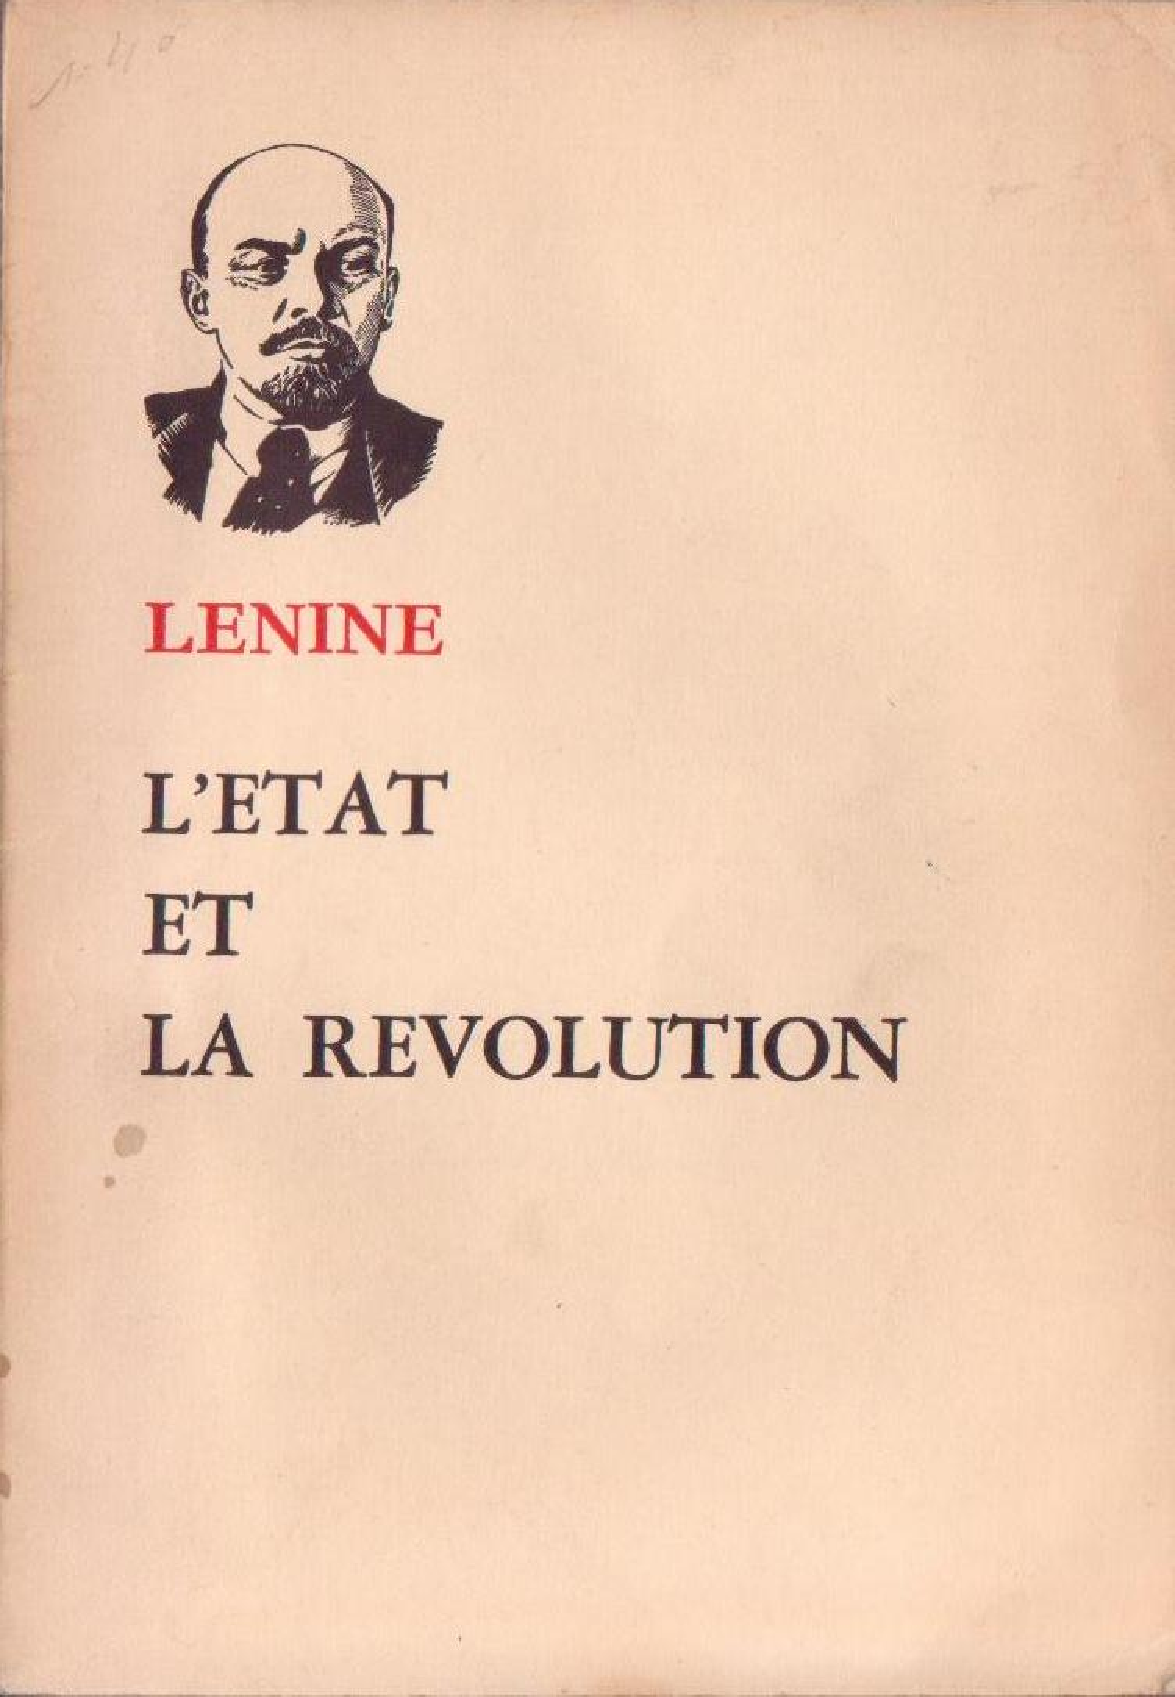
\includepdf[pagecommand={\thispagestyle{empty}}]{episode/FrontPage} 
\clearpage\thispagestyle{empty}\cleardoublepage

% 标题页
% 标题页

\leftskip=5mm
\small
\mbox{} \mbox{}

{\kaishu 全世界无产者,联合起来!}

\mbox{} \mbox{}

\leftskip=0mm
\begin{center}	
	\Large \kaishu{列~~宁}  \par 
	
	\huge{\Fheiti 国~~家~~与~~革~~命~~} \pskip
	
	\normalfont{}
	\normalsize
	
	(马克思主义关于国家的学说与\par 无产阶级在革命中的任务)$^{1}$
	
	\vfill
	
	\zihao{5}
	人~~~~民~~~~出~~~~版~~~~社
	
	一九六〇年$\cdot$ 北京	
\end{center}
\thispagestyle{empty}
\clearpage
%\bookmark[page=2,level=0]{封页}

% 出版信息页
% 出版信息页
\begin{center}
		
	\zihao{4}\fangsong\mbox{}
	
	\mbox{}\label{publish}\pdfbookmark{出版页}{publish}
	
	В.И.Ле́нин
	
	ГОСУДАРСТВО
	
	И 
	 
	РЕВОЛЮЦИЯ
	
	{\small 根据“列宁全集”中文版第25卷中的译文拓印。}
	
	\vfill \normalsize \kaishu{列~~宁} 
	
	\Fheiti{国~~家~~与~~革~~命~~}
	
	\normalfont{} 
	*
	
	人民出版社出版
	
	\zihao{-5} (北京朝阳门火街320号)
	
	\normalsize 
	北京外文印刷厂印刷~~新华书店总经营
	
	
	*
	
	\zihao{6}开本:850$\times$1168~~公厘$\frac{1}{32}$ $\cdot$印张:$3\frac{3}{4}$ $\cdot$字数:32,000
	
	1949年8月第1版~~~~1959年9月第6版
	
	1960年9月北京第8次印刷
	
	\normalsize 统一书号:1001$\cdot$21~~~~定价(四)0.33元
\end{center}
\thispagestyle{empty}
\clearpage


\frontmatter

%目录
\pagestyle{plain}
\tableofcontents 
\clearpage\thispagestyle{empty}\cleardoublepage

\mainmatter

\pagestyle{headings}

%\part[初版序言]{初\quad 版\quad 序\quad 言} % 初版序言 初\quad 版\quad 序\quad 言
\clearpage\thispagestyle{empty}\cleardoublepage % 单独留出一空白页

\chapter[初版序言]{初~版~序~言} % 小章节名称
%\blfootnote{} % 底线批注
%\pskip % 跳大行,段落间用
%\noindent % 书信体的开头
%\mbox{} % 插入个盒子,设定好的大小,用于隔开文本
%\leftskip= 文本左边腾出空格,用于文本排版


国家问题,现在无论在理论方面或在政治实践方面,都具有特别重大的意义。帝国主义战争大大加速和加剧了垄断资本主义变为国家垄断资本主义的过程。国家同拥有无限权力的资本家集团日益密切地溶和在一起,它对劳动群众的残酷压迫,愈来愈骇人听闻了。各先进国家(我们在这里是指这些国家的“后方”而言)已经变成了囚禁工人的军事苦工监狱。

连绵不断的战争造成的空前惨剧和灾难,使群众生活困苦不堪,使他们更加义愤填膺。国际无产阶级革命正在显著地发展,这个革命对国家所抱的态度,已经成为具有实际意义的问题了。

在几十年较为和平的发展中积聚起来的机会主义成分,使得社会沙文主义流派在世界各个正式社会主义政党内取得了统治地位。这个流派(在俄国有普列汉诺夫、波特列索夫、布列什柯夫斯卡娅、鲁巴诺维奇以及不太露骨的策列铁里先生、切尔诺夫先生之流;在德国有谢德曼、列金、大卫等;在法国和比利时有列诺得尔、盖德、王德威尔得;在英国有海德门和费边社分子$^{2}$等等)口头上是社会主义,实际上是沙文主义,其特点就在于这些“社会主义领袖”不仅对于“自己”民族资产阶级的利益,而且正是对于“自己”国家的利益,采取卑躬屈膝的迎合态度。因为大多数所谓大国早就在剥削和奴役很多弱小民族,帝国主义战争也正是为了瓜分和重分这些赃物而进行的战争。如果不在“国家”问题上反对机会主义偏见,就不能展开斗争,不能使劳动群众摆脱资产阶级的影响,特别是摆脱帝国主义资产阶级的影响。

首先,我们来考察一下马克思和恩格斯的国家学说,特别详细地谈谈这个学说被人遗忘或者遭到机会主义者歪曲地各个方面。其次,我们要专门分析一下歪曲这个学说地主要代表人物,即在这次战争中可耻地遭到彻底破产的第二国际(1889-1914年)最著名的领袖考茨基。最后,我们要给俄国1905年革命、特别是1917年革命的经验,做一个基本的总结。后面这次革命的第一个阶段现在(1917年8月初)大概正在结束,但整个这次革命只能认为使帝国主义战争引起的社会主义无产阶级革命的链条中的一个环节。无产阶级社会主义革命对国家的态度问题向群众说明,为了使自己从资本的枷锁下解放出来,他们在最近的将来应该做些什么。因此这个问题不仅具有实际的政治意义,而且具有最迫切的意义。

\mbox{} 

\leftskip=80mm 作者

\leftskip=73mm 1917年8月

\leftskip=0mm

%\clearpage\thispagestyle{empty}\cleardoublepage % 单独留出一空白页
%\part[再版序言]{再\quad 版\quad 序\quad 言} % 再版序言
%\clearpage\thispagestyle{empty}\cleardoublepage
%\leftskip=0pt % 恢复初始格式设置

\chapter[再版序言]{再~版~序~言} % 小章节名称
%\blfootnote{} % 底线批注
%\pskip % 跳大行,段落间用
%\noindent % 书信体的开头
%\mbox{} % 插入个盒子,设定好的大小,用于隔开文本
%\leftskip= 文本左边腾出空格,用于文本排版


本书再版时几乎没有变动,仅在第二章中增加了第三节

\mbox{} 

\leftskip=80mm 作者

\leftskip=73mm 1917年8月

\clearpage\thispagestyle{empty}\cleardoublepage

% 第一章 阶级社会和国家
\part[第一章]{第~一~章 \\ 阶级社会和国家}  
%\clearpage\thispagestyle{empty}\cleardoublepage
\leftskip=0pt

\chapter{国家是阶级矛盾不可调和的产物} % 小章节名称
% \blfootnote{} % 底线批注,在所需段落前加入
% \pskip % 跳大行,段落间用
% \noindent % 书信体的开头
% \mbox{} % 插入个盒子,设定好的大小,用于隔开文本
% \leftskip= 文本左边腾出空格,用于文本排版
% \CJKunderdot{} % 文字下加点
% {\kaishu } % 更改字体为楷书


马克思的学说在今天的遭遇,正如历史上各被压迫阶级解放斗争中的革命思想家和领袖的学说的遭遇一样。当伟大的革命家在世时,压迫阶级总是不断迫害他们,以最恶毒的敌意、最疯狂的仇恨、最放肆的诽谤对待他们的学说。在他们逝世以后,便企图把他们变为无害的神像,即所谓把他们偶像化,赋予他们的{\kaishu 名字}某种荣誉,以便“安慰”和愚弄被压迫阶级,同时却阉割革命学说的内容,磨灭它的革命锋芒,把它庸俗化,这同现在资产阶级和工人运动中的机会主义对马克思主义作的这种“修改”是一致的。他们遗忘、抹杀和歪曲这个学说的革命方面和革命精神,把资产阶级可以接受或者似乎可以接受的东西放在第一位来加以颂扬。现在,一切社会沙文主义者都成了“马克思主义者”(请不要笑!)。那些德国的资产阶级学者,昨天还是摧残马克思主义的专家,现在却愈来愈频繁地谈论起“德意志民族的”马克思来了,仿佛马克思培育极有组织的工人协会是为了进行掠夺战争!

在这种情况下,在歪曲马克思主义的风气空前流行的时候,我们的任务首先就是要{\kaishu 恢复}马克思关于国家的真正学说。为此,必须引证马克思和恩格斯著作中的许多话。当然,很多的引证会使文章冗长,不通俗,但是没有这样的引证是绝对不行的。马克思和恩格斯著作中所有论到国家问题的地方,至少一切有决定意义的地方,我们要尽可能完整地加以引证,一方面是读者对科学社会主义创始人的整个观点以及这些观点的发展有一个独立的概念,同时也可以确切地证实并指明现在占统治地位地“考茨基主义”对这些观点的歪曲。

我们现在先从传播最广的恩格斯的著作“家庭、私有制和国家的起源”一书讲起,这本书于1894年在斯图加特印行了第六版。我们必须根据德文原著译出一段引文,该书俄文译本虽然很多,但多半译得不完全,或者译得很糟。

\pskip
\leftskip=10mm
\small
恩格斯在总结他所做得历史分析时说:“国家绝不是从外面强加于社会得一种力量。国家也不想黑格尔所断言的是‘道德观念的现实’或‘理性的形象和现实’。国家是社会发展到一定阶段的产物;国家是社会陷入自身不可解决的矛盾的表现,是社会分裂为不可调和的对立面而又无力摆脱这种对立情况的表现。为了使这些对立面——这些经济利益彼此冲突的阶级不致在无谓的斗争中互相消灭,使社会同归于尽,于是,一种似乎驾于社会之上的力量,似乎可以缓和冲突、使它不致破坏‘秩序’的力量,就成为必要了。这个从社会中产生、驾于社会之上并日益同社会脱离的力量,就是国家。”(德文第六版第177-178页)$^{3}$

\leftskip=0mm
\normalsize
\pskip
这一段话已经十分清楚地表明了马克思主义关于国家的历史作用及其意义的基本思想。国家使阶级矛盾{\kaishu 不可调和}的产物和表现。在阶级矛盾客观上达到{\kaishu 不能调和}的地方、时候和程度,便产生国家。反过来说,国家的存在表明阶级矛盾的不可调和。

正是在这个最重要的根本问题上,人们从两个主要方面来歪曲马克思主义。

一方面,资产阶级的思想家,贴别是小资产阶级的思想家,迫于无可辩驳的历史事实而不得不承认,只有在有阶级矛盾和阶级斗争的地方才有国家,但他们又来“改正”马克思,说国家是阶级{\kaishu 调和}的机关。在马克思看来,如果阶级调和是可能的话,国家就不会产生,也不会保持下去。在市侩的庸俗的教授和政论家们(他们往往善意地引用马克思的言论!)看来,国家正是用来调和阶级的。在马克思看来,国家是阶级{\kaishu 统治}的机关,是一个阶级{\kaishu 压迫}另一个阶级的机关,是建立一种“秩序”,来使这种压迫合法化、固定化,使阶级冲突得到缓和。在小资产阶级政治家看来,秩序正是阶级调和,而不是一个阶级压迫另一个阶级;缓和冲突就是调和,而不是剥削被压迫阶级用来推翻压迫者的一定的斗争工具和手段。

\blfootnote{[1] 孟什维克(меньшевик),是地处欧洲东部和亚洲北部的俄国早期工人运动中的资产阶级改良主义派别}
例如,在1917年革命的时候,对国家的意义和作用的看法是一个非常重要的问题,是需要在实践中立刻行动,而且是大规模行动的问题,全体社会革命党人和孟什维克$^{[1]}$在这个问题上一下子就完全滚到“国家”“调和”阶级的小资产阶级理论方面去了。这两个政党的无数决议和他们的政治家的许多论文,都浸透了这种市侩的庸俗和“调和”论。国家是一定阶级的统之机关,这个阶级{\kaishu 绝不能}与同它对立的一方(同它对抗的阶级)调和,这一点是小资产阶级民主派始终不能了解的。在对待国家的态度问题上,再明显不过地表明我国社会革命党人和孟什维克根本不是社会主义者(我们布尔什维克向来就这样说),而是唱准社会主义高调地小资产阶级民主派。

另一方面,“考茨基主义”歪曲马克思主义地方法就巧妙得多了。“在理论上”,它不否认国家是阶级统治的机关,也不否认阶级矛盾是不可调和的。但是,它忽视或抹杀了一下一点:既然国家是阶级矛盾不可调和的产物,既然它是驾于社会之上并“\CJKunderdot{\kaishu 日益}同社会\CJKunderdot{\kaishu 脱离}”的力量,那么很明显,被压迫阶级的解放,不仅非暴力革命不可,\CJKunderdot{\kaishu 而且非消灭}统治阶级建立的、体现这种“脱离”的国家政权机关不可。这个结论在理论上是不言而喻的,西面我们会看到,这是马克思对革命的任务做了具体的历史分析后得出的绝对肯定的结论。正是这个结论(我们在下面还要详细说明)竟被考茨基······“遗忘”和歪曲了。




 % 国家是阶级矛盾不可调和的产物
\chapter{特别的武装队伍,监狱等等} % 小章节名称
%\blfootnote{} % 底线批注,在所需段落前加入
%\pskip % 跳大行,段落间用
%\noindent % 书信体的开头
%\mbox{} % 插入个盒子,设定好的大小,用于隔开文本
%\leftskip= 文本左边腾出空格,用于文本排版
% \CJKunderdot{} % 文字下加点
% {\kaishu } % 更改字体为楷书

恩格斯又说:
\pskip
\leftskip=10mm
\small

······“国家同旧的氏族(或宗族)组织不同的第一个特征,就是它按地域来划分它统治下的国民”······

\leftskip=0mm
\normalsize
\pskip

我们现在看来,这种划分是“很自然的”,但是这是同宗族或氏族的旧组织进行长期斗争获得的。

\pskip
\leftskip=10mm
\small

······“第二个特征,就是社会权力的建立,这个权力已经不是自己组织成武装力量的居民了。这个特别的社会权力之所以需要,是因为自从社会分裂成阶级以后,已经不可能有居民自动组成的武装了······\quad 这个社会权力在每一个国家里都有存在。构成这个权力的不仅有武装队伍,还有监狱、各种强制机关等物质附属机构,这些东西都是以前氏族社会制度没有的” ······

\leftskip=0mm
\normalsize
\pskip

恩格斯在这里阐明了由社会中产生而驾于社会之上并日益同社会脱离的国家这个力量的概念。这个力量主要是指什么呢?主要是指有用监狱等等的特别武装队伍。

应该说这是特别的武装队伍,因为任何国家所具有的社会权力已经不是武装的居民,不是居民“自动组成的武装”了。

同一切伟大的革命思想家一样,恩格斯竭力促使党悟工人注意的,正是盛行的庸俗观念认为最不值得注意、最习以为常,而被根深蒂固的,可以说是国家的权力的主要的工具,但是——难道可能不是这样吗?

\blfootnote{[2] 赫伯特·斯宾塞(Herbert Spencer,1820-1903)——“社会达尔文主义之父”、进化论先驱}
\blfootnote{[3]米海洛夫斯基(Н.К)——俄国社会学家、政治家,自由主义民粹派的著名代表,俄国主观社会学的创始人之一}
19世纪末叶,绝大多数欧洲人认为,这是不能不这样的。恩格斯的话正是对这些人说的。他们没有经历过,也没有亲眼看到过一次伟大的革命,他们完全不了解,什么是“居民自动组成的武装”。对于为什么要有驾于社会之上并使自己同社会脱离的特别武装队伍(警察、常备军),西欧和俄国的庸人总是喜欢借用斯宾塞$^{[2]}$和米海洛夫斯基$^{[3]}$的几句话来答复,说这是因为社会生活复杂化、职能分化等等。

这种说法似乎是“科学的”,而且最能迷惑庸人,掩盖社会分裂为不可调和敌对阶级这个主要的基本的事实。

如果没有这种分裂,“居民自动组成的武装”同使用棍棒的猿猴群、原始人类,或宗族社会的原始组织比较起来,只是程度上复杂些,技术上高明些,但这样的武装组织是可能的。

这样的组织之所以不可能有,就因为文明社会已分裂为敌对的而且是不可调和地敌对的阶级,如果这些阶级都有“自动组成的”武装,那在它们之间就一定会展开武装斗争。于是国家形成了,特别的力量、特别的武装队伍建立起来了。每当革命破坏国家机关的时候,我们都能清楚地看到,统治阶级是如何力图恢复替\CJKunderdot{\kaishu 它} 服务的特别武装队伍,被压迫阶级又是如何力图建立一种不替剥削者服务,而替被剥削者服务的新型组织。

上面恩格斯从理论上提出的问题,即每次大革命在实践中明显地而且是以大规模的行动提到我们面前的问题。正是“特别”武装队伍同“居民自动组成的武装”之间的相互关系问题。我们会看到,欧洲和俄国历次革命的经验是怎样具体地说明这个问题地。

现在我们再来看看恩格斯的论述。

他指出,有的时候,如在北美某些地方,这种社会权力是薄弱的(这里指的只是资本主义社会中少数的例外,以及在帝国主义时期以前北美那些自由移民占多数的地方),但一般说来,它是在加强:

\pskip
\leftskip=10mm
\small

······“社会权力是随着国家内部阶级矛盾尖锐化及邻国的扩大和人口增多而加强起来的。拿现在的欧洲来说,阶级斗争和侵略竞争已把社会权力提高到可以吞食整个社会,甚至吞食整个国家的地步” ······

\leftskip=0mm
\normalsize
\pskip

\blfootnote{[4]托拉斯(英语:Trust)是商业信托的音译,垄断组织的高级形式之一。}
这段话至迟是在19世纪90年代初期写的。恩格斯最后的序言写于1891年6月16日。当时向帝国主义的转变,无论就托拉斯$^{[4]}$的完全统治、大银行的无限权力或大规模的殖民政策等等来说,在法国还是刚刚开始,在北美和德国要差一点。此后,“侵略竞争”前进了一大步,尤其因为到了20世纪20年代初,世界已被这些“互相竞争的侵略者”,即巨大的强盗国家瓜分完了。从此海陆军备无限增长,1914年至1917年英德两国为了争夺世界霸权、为了瓜分赃物而进行的强盗战争,使社会上一切力量几乎都被强盗国家政权“吞没”,使情况发展到不可收拾的地步。

恩格斯在1891年就已指出,“侵略竞争”是各大强国对外政策最重要的特征之一,但是社会沙文主义的恶棍们在1914年至1917年,正当这个竞争加剧了许多倍并引起了帝国主义战争的时候,却用“保卫祖国”、“保卫共和国的革命”等等词句来掩盖他们维护“自己”资产阶级强盗利益的行为!





 % 特别的武装队伍,监狱等等
\chapter{国家是剥削和被压迫阶级的工具} % 小章节名称
%\blfootnote{} % 底线批注,在所需段落前加入
%\pskip % 跳大行,段落间用
%\noindent % 书信体的开头
%\mbox{} % 插入个盒子,设定好的大小,用于隔开文本
%\leftskip= 文本左边腾出空格,用于文本排版
% \CJKunderdot{} % 文字下加点
% {\kaishu } % 更改字体为楷书

为了维持驾于社会之上的特别社会权力,就需要捐税和国债。

\pskip
\leftskip=10mm
\small

恩格斯说:“官吏既然掌握着社会权力和征税权,他们就会成为社会机关而驾于社会之上。从前人们对氏族(或宗族)社会机关的那种自愿的敬意,即使他们能够获得,也不能使他们满足了。”······于是制定了官吏是神圣不可侵犯的特别法律。“一个微不足道的警察”却有大于氏族代表的“权威”,然而,即使是文明国家掌握军权的首脑,也会对“不是用强迫手段获得社会尊敬”的氏族首领表示羡慕。

\leftskip=0mm
\normalsize
\pskip

这里提出了作为国家政权机关的官吏的特权地位问题。指出了这样一个基本问题:究竟什么东西使他们驾于社会之上?我们在下面就会看到,1871年巴黎公社如何实际地解决了这个理论问题,而在1912年又如何被考茨基反动地抹杀了。

\pskip
\leftskip=10mm
\small

······“因为国家是为了控制阶级对抗而产生的,同时又是在这种阶级冲突中产生的,所以,它照例是最强大的、在经济上占统治地位的阶级的国家,这个阶级借助与国家而在政治上也成为占统治地位的阶级,因而获得了压制和剥削被压迫阶级的新手段”······不仅古代的国家和封建国家是剥削奴隶和农奴的机关,“现代的代议制国家也是资本剥削雇佣劳动的工具。但是也常有一些例外,如相互斗争的阶级达到势均力敌的地步,国家政权就暂时获得某种独立性,似乎成了这两个阶级之间的中介人”······17世纪和18世纪的君主专制,法国第一帝国和第二帝国的拿破仑主义,德国的俾斯麦时代,都是如此。

\leftskip=0mm
\normalsize
\pskip

\blfootnote{[5]亚历山大·弗多洛维奇·克伦斯基(А.В Керенский,1881-1970)——俄社会革命党人,发动二月革命。}
我们还可补充说,在共和制俄国的克伦斯基$^{[5]}$政府还是压迫革命无产阶级以后,由于小资产阶级民主派的领导,苏维埃{\kaishu 已经}软弱无力,而资产阶级{\kaishu 还}没有足够的力量来直接解散苏维埃的时候,也如此。

\pskip
\leftskip=10mm
\small

恩格斯又说,在民主共和国内,“财富是间接地发挥它的权力地,因此是更可靠的”,它所采用地第一个方法是“直接收买官吏”(美国),第二个方法是“政府同交易所结合”(法国和美国)。

\leftskip=0mm
\normalsize
\pskip

\blfootnote{[6]法文译词(syndicat),原意是“组合”,是垄断组织的重要形式之一}
\blfootnote{[7]上述人物为社会革命党或孟什维克派人士}
目前,任何最民主地共和国中地帝国主义和银行统治,都把这两种维护和实现财富地无限权力地方法“发展”到了非常巧妙地地步。例如,在俄国实行民主共和的头几个月里,在社会革命党人和孟什维克这两种“社会主义者”同资产阶级联姻的“蜜月”期间,帕尔钦斯基先生在联合政府中实行怠工,不愿实施制裁资本家、制止他们进行掠夺和借军事订货盗窃国库的种种措施,在帕尔钦斯基先生退出内阁以后(接替他的自然是同他一模一样的人),资本家“奖赏”给他年薪12万卢布的肥缺,试问这究竟是怎么一回事呢?是直接的收买,还是间接的收买?是政府同辛迪加$^{[6]}$勾结,还是“仅仅”是一种友谊关系?切尔诺夫、策烈铁里、阿夫克森齐耶夫、斯柯别列夫$^{[7]}$之流究竟起着什么作用?他们是盗窃国库的百万富翁的“直接”同盟者,还是仅仅是间接的同盟者?

“财富”的无限权力在民主共和制度下之所以更{\kaishu 可靠},是因为它不依赖资本主义的不好的政治外壳。民主共和制度是资本主义所能采用的最好的政治外壳,所以资本一掌握(通过帕尔钦斯基、切尔诺夫、策烈铁里之流)这个最好的外壳,就能十分可靠十分巩固地确立自己地权力,在资产阶级民主共和国中,无论人员、机关或政党地{\kaishu 任何}更换,都不会使这个权力动摇。

还应该指出,恩格斯十分肯定地认为,普选制是资产阶级统治的工具。他显然是估计了德国社会民主党的长期经验,他说普选制是
\pskip
\leftskip=10mm
\small

“工人阶级成熟的指标。在现代国家,普选制不能而且永远不会提供更多的东西”。

\leftskip=0mm
\normalsize
\pskip

小资产阶级民主派,如我国社会革命党人和孟什维克,及其同胞兄弟西欧一切社会沙文主义者和机会主义者,都希望从普选制中得到“更多的东西”。他们自己相信而且要人民也相信这种荒谬的想法,似乎普选制“在{\kaishu 现代}国家中”真正能够体现大多数劳动者的意志,并保证实现这种意志。

我们在这里只是指出这个错误的想法,只是指出,恩格斯这个十分明确而具体的说明,经常在“正式的”(即机会主义的)社会主义政党的宣传活动中遭到歪曲。至于恩格斯如何揭露这种想法的全部虚伪性,我们以后在谈到马克思和恩格斯对“{\kaishu 现代}”国家的看法时,还会详细地加以阐明。

恩格斯在他那部最通俗的著作中,把自己的看法总结如下:
\pskip
\leftskip=10mm
\small

“由此可见,国家不是自古就有的。曾经有过不需要国家、而且根本不知国家和国家政权为何物的社会。在经济发展到一定阶段而必然使社会分裂为几个阶级时,国家就成为必要了。现在我们正以迅速的步伐走上这样的生产发展阶段,在这个阶段上,这些阶级的存在不仅已经没有必要,而且成了生产的直接障碍。阶级必然会消失,正如他们从前必然会产生一样。随着阶级的消失,国家也必然会消灭。以生产者自由平等的联合体为基础的,按新方式来组织生产的社会,将把全部国家机器放到它应该去的地方,即放到古物陈列馆去,同纺车和青铜斧陈列在一起。”

\leftskip=0mm
\normalsize
\pskip

这一段引文在现代社会民主派的宣传鼓动书刊中很少看到,即使引用也多半是为了崇拜偶像,也就是说,为了正式表示对恩格斯的尊敬。他们根本不去考虑,先要经过怎样广泛而深刻的革命,才能“把全部国家机器放到古物陈列馆去”。甚至他们往往不懂恩格斯说的国家机器是什么。





 % 国家是剥削和被压迫阶级的工具
\chapter{国家“消亡”和暴力革命} % 小章节名称
%\blfootnote{} % 底线批注,在所需段落前加入
%\pskip % 跳大行,段落间用
%\noindent % 书信体的开头
%\mbox{} % 插入个盒子,设定好的大小,用于隔开文本
%\leftskip= 文本左边腾出空格,用于文本排版
% \CJKunderdot{} % 文字下加点
% {\kaishu } % 更改字体为楷书

恩格斯关于国家“消亡”的话是非常著名的,经常有人引证,它清楚地表明了目前流行的把马克思主义偷偷地改为机会主义的把戏的本质,因此我们必须详细地加以说明。现在我们把这句话的出处的那一段论述转录如下:

\leftskip=10mm
\small

“无产阶级取得了国家政权,首先把生产资料变为国家财产。按这样一来,无产阶级就消灭了自己之为无产阶级,就消灭了一切阶级差别和阶级对立,同时也就消灭了国家之为国家。过去和现在在阶级对立中向前发展的社会,需要国家,即需要一个剥削阶级的组织,以便维持其生产的全部外部条件,特别是用强力把被剥削阶级控制在当时生产方式所决定的那些压迫条件(奴隶制、农奴制、雇佣劳动制)以内。国家会是整个社会的正式代表,是社会的集中组织形式,但是国家所以成为这样,只是因为它是当时唯一代表整个社会的阶级的国家。在古代,它是奴隶主即国家公民的国家;在中世纪,它是封建贵族的国家;在我们的时代,它就自然而然地成为多余的东西了。那时候,必须加以镇压的社会阶级已不存在,一个阶级统治另一个阶级的现象以及目前生产无政府状态引起的生存斗争已不然存在,这个斗争中的冲突和过火行动(极端化)也随着消失,再也没有什么东西须要镇压了,于是,实行镇压的特别力量——国家也就不需要了。国家作为全社会的真正代表而采取的第一个行动,即以社会名义占有生产资料,也就是它以国家资格所采取的最后一个独立行动。那时,国家政权对社会关系的干涉,便会逐步成为多余的东西而自行停止。对人的管理将由对物的管理和对生产过程的指导所代替。国家不是‘被废除’的,它是自行消亡的。应该根据这一点来评价‘自由的人民国家’这句话,这句话用来鼓动暂时还可以,但毕竟是没有科学依据的。同时也应该根据这一点来评价所谓无政府主义者要在一天之内废除国家的要求。”(“反杜林论”德文第三版第301-303页)$^{4}$

\pskip
\leftskip=0mm
\normalsize

我们可以大胆地说:在恩格斯这一段思想极其丰富地论述中,只有与无政府主义“废除”国家地学说不同地国家“消亡”(马克思语)这一点,被现代社会主义政党当作真正的社会主义思想接受下来了。这样来割裂马克思主义,无异是把马克思主义编程机会主义,这样来“解释”,就只会留下一个模糊的观念,似乎只有缓慢的、平静的、逐渐的变化,而没有突变、风暴和革命。对国家“消亡”最普遍、最流行、最大众化的(如果能这样说的话)理解,无疑是抹杀革命,甚至是否认革命。

但是,这样的“理解”是对马克思主义的最粗暴的歪曲,仅仅有利于资产阶级。从理论上讲,产生这种歪曲的根源就是忘记了我们上面全部摘引的恩格斯的“总结性”论述中所指出的极重要的情况和观点。

第一、恩格斯在这段论述中一开始就说,无产阶级取得了国家政权,“也就消灭了国家之为国家”。这句话究竟是什么意思,人们“照例”是不假思索的,他们不是完全忽略这一点,就是认为这是恩格斯的“黑格尔主义的毛病”。其实这几句话扼要地表明了最伟大的一次无产阶级革命的经验,即1871年巴黎公社的经验,关于这一点,我们在下面还要详细地加以论述。实际上恩格斯在这里所讲的是以无产阶级革命来“消灭”{\kaishu 资产阶级}的国家,他讲的消亡是指社会主义革命{\kaishu 以后的无产阶级}国家制度的残余。恩格斯认为资产阶级国家是不会“自行消亡”的,而是要用无产阶级革命来“\CJKunderdot{\kaishu 消灭}”它。在这个革命以后,自行消亡的是无产阶级的国家或半国家。

第二、国家是“实行镇压的特别力量”,恩格斯下的这个绝妙而极其深刻的定义是十分明确的。从这个定义可以得出这样的结论:资产阶级对无产阶级,即一小撮富豪对千百万劳动者“实行镇压的特别力量”,应该由无产阶级对资产阶级“实行镇压的特别力量”(无产阶级专政)来代替。这就是“消灭国家之国家”。这就是以社会名义占有生产资料的“行动”。显然,以无产阶级的“特别力量”来代替资产阶级的“特别力量”,这样一种更换是绝不能靠“自行消亡”来实现的。

第三、恩格斯在谈到“自行消亡”和更鲜明更光辉的“自行停止”一语时,他十分明确而肯定地说,这是指在“国家以社会名义占有生产资料”\CJKunderdot{\kaishu 以后},即在社会主义革命\CJKunderdot{\kaishu 以后} 的事情。我们大家都知道,这时“国家”的政治形式是最彻底的民主制。但是那些无耻地歪曲马克思主义的机会主义者,却没有一个人想到恩格斯在这里所说的就是\CJKunderdot{\kaishu 民主制} 的“自行停止”和“自行消亡”。乍看起来,这似乎是很奇怪的。但是,只有那些没有想到民主制\CJKunderdot{\kaishu 也} 是国家、在国家消逝时民主制也会消逝的人,才会觉得这是“不可理解”的。资产阶级的国家只有革命才能“消灭”。最彻底的民主国家只能“自行消亡”。

第四、恩格斯在提出“国家自行消亡”这个著名的原理以后,立刻就具体地说明这一点时既反对机会主义者又反对无政府主义者的。但恩格斯放在首位的,是从这个原理中得出的反对机会主义者的结论。

可以担保,在1万个读过或听过“国家自行消亡”的论述的人中,由9990人完全不知道或不记得恩格斯从这个原理中得出的结论{\kaishu 不仅}是反对无政府主义者的。其余的10个人中可能有9个人不懂得什么是“自由的人民国家”,不懂得为什么反对这个口号就是反对机会主义者。历史就是这样记载的!伟大的革命学说就是这样被人偷偷地改成了流行的庸人主义!人们千百次地重复反对无政府主义者地结论,把它庸俗化并简单地装到头脑中去,形成了固执的偏见。至于反对机会主义者的结论,却被抹杀和“忘记”了!

“自由的人民国家”是70年代德国社会民主党人提出的纲领性要求和流行口号。这个口号只是市侩式地夸大了民主制的概念,没有丝毫政治内容。既然人们当时可以合法地利用这个口号来暗示民主共和国,恩格斯也就从鼓动的观点同意“暂时”替这个口号“辩护”。但这是一个机会主义的口号,它不仅起了粉饰资产阶级民主共和制的作用,而且表现出不懂得社会主义对一般国家的批评。我们拥护民主共和国,因为在资本主义制度下这是对无产阶级最有利的国家形势,但是,我们绝不能忘记,即使在最民主的资产阶级共和国里,人民仍然摆脱不了当雇佣奴隶的命运。在任何国家都是对被压迫阶级“实行镇压的特别力量”。因此{\kaishu 任何}国家都{\kaishu 不是}人民的。在70年代,马克思和恩格斯一再向他们党内的同志解释这一点。

第五、在恩格斯这本著作中,除了大家记得的关于国家消亡的论述以外,还谈到了暴力革命的意义。恩格斯对于革命的作用的历史评价成了对暴力革命的真正颂扬。但是,“谁都不记得”这一点,这个思想的意义在现代社会政党内是照例不谈、照例不想的,在群众进行的日常鼓动宣传中也不占任何地位。其实,这个思想同国家“自行消亡”的理论是密切联系的,是一个严密的整体。

请看恩格斯的论述:
\blfootnote{[8]“反杜林论”1956年人民出版社第190页}
\pskip
\leftskip=10mm
\small

······“暴力在历史上还起着另一种作用”(除作恶以外)“即革命的作用,暴力是替代任何一个孕育着新社会的旧社会接生的产婆(马克思语),暴力是社会运动借以开辟道路并破坏僵死硬化的政治形势的工具和手段,——关于这一切,杜林先生一个字也没有提到。他仅仅带着叹息和呻吟的口吻承认,为了推翻剥削者的经营制度,暴力也许是必要的(你们看,真可惜!),而任何暴力的采用,据说都会使采用暴力的人道德坠落。尽管在每次革命胜利以后,道德和思想都有显著的提高,他还是说出来这种话!而且这是在德国说的,当时德国人民可能被迫进行暴力冲突,发生这种事件的好处至少是可以排除三十年战争的耻辱在民族意识中造成的奴才气。难道可以把这种灰色的、萎靡不振、软弱无力的僧侣思想,推荐给历史上最革命的政党吗?”(“反杜林论”德文第三版第193页;第二编第四章末)$^{[8]}$

\pskip
\leftskip=0mm
\normalsize

怎样才能把恩格斯从1878年起至1894年他逝世时为止,一再向德国社会民主党人提出的颂扬暴力革命的论点,同国家“消亡”的理论结合起来呢?

人们往往用折衷主义,用无原则地或诡辩式地任意(或者为了讨好当权者)抽出前者或后者地方法把它们结合起来,而且在100次中有99次(如果不是更多的话)正是把国家“消亡”论摆在首位,用折衷主义代替辩证法,这就是目前在正式的社会民主党书刊中对马克思主义采取的最常见的最普遍的手法。这种做法,自然并不新奇,甚至在希腊古典哲学史上也是常见的。把马克思主义偷偷地改为机会主语的时候,用折衷主义冒充辩证法是最容易欺骗群众的。这样能使人感到一种似是似非的满足,似乎考虑到了过程的一切方面,发展的一切趋势,各方面的矛盾的影响等等,但实际上并没有对社会发展过程做出任何完整的革命分析。

我们在前面已经说过,马克思和恩格斯关于暴力革命不可避免的学说使针对资产阶级国家说的,在下面我们还要更详细地说明这一点。资产阶级国家由无产阶级国家(无产阶级专政)代替是{\kaishu 不能}经过“自行消亡”来实现的。根据一般规律,只能靠暴力革命来实现。恩格斯对暴力革命的颂扬同马克思的屡次声明完全符合(我们可以回忆一下,马克思在“哲学的贫困”$^{5}$和“共产党宣言”$^{6}$这两部著作的结尾部分,曾自豪地公开生命暴力革命的必然性;我们还可以回忆一下,约在30年以后,马克思在1875年写的“哥达纲领批判”$^{7}$中,曾无情地抨击了这个纲领表现的机会主义),这种颂扬决不是“迷恋”,决不是夸张,也决不是论战伎俩。必须不断教育群众,使他们{\kaishu 这样}来认识暴力革命,而且只能这样来认识暴力革命;这正是马克思和恩格斯{\kaishu 全部}学说的基础。现在占统治地位的社会沙文主义和考茨基主义流派对马克思和恩格斯学说的背叛,最突出地表现在这两个流派都把{\kaishu 这方面}的宣传和鼓动忘记了。

无产阶级国家代替资产阶级国家,必须通过暴力革命。无产阶级国家的消灭,即任何国家的消灭,只能通过“自行消亡”。

马克思和恩格斯在研究每一个革命形势,分析每一个革命的经验教训时,总是详细而具体地发挥了他们的这些见解。我们现在就来谈谈他们学说中这个最重要的部分。











 % 国家“消亡”和暴力革命

%\clearpage\thispagestyle{empty}\cleardoublepage

% 第二章 国家与革命 1848-1851年的经验
\part[第二章]{第~二~章 \\ 国家与革命\\ 1848-1851年的经验}  
%\clearpage\thispagestyle{empty}\cleardoublepage

\chapter{革命的前夜} % 小章节名称
%\blfootnote{} % 底线批注,在所需段落前加入
%\pskip % 跳大行,段落间用
%\noindent % 书信体的开头
%\mbox{} % 插入个盒子,设定好的大小,用于隔开文本
%\leftskip= 文本左边腾出空格,用于文本排版
% \CJKunderdot{} % 文字下加点
% {\kaishu } % 更改字体为楷书

成熟的马克思主义的最初著作“哲学的贫困”和“共产党宣言”,恰巧是在1848年革命前夜写成的。由于这种情况,这两本书除了叙述马克思主义的一般原理外,还在一定程度上反映了当时具体的革命形势。因此,我们来研究这两部著作的作者在做出1848-1851年革命经验的总结以前关于国家问题的言论,也许更为恰当。

\pskip
\leftskip=10mm
\small

马克思在“哲学的贫困”中写道,······“工人阶级在发展进程中将创造一个没有阶级和阶级对立的联合体来代替旧的资产阶级社会;从此再不会有任何原来意义的政权了,因为政权正是资产阶级社会内阶级对抗的正式表现。”(1885年德文版第182页)$^{8}$

\leftskip=0mm
\normalsize
\pskip

拿马克思和恩格斯在几个月后(1847年11月)写的“共产党宣言”中的论述来同这一段关于国家会随着阶级消灭而消逝的思想的论述比较一下,是颇有教益的。

\pskip
\leftskip=10mm
\small

······“当我们叙述无产阶级发展中最一般的阶段时,我们探讨了现存社会里多少带有隐蔽性的国内战争,一直到这个国内战争变成公开的革命,那是无产阶级就用暴力推翻资产阶级而建立自己的统治”······

······“我们在前面已经看见,工人革命的第一步是无产阶级变为(直译是提升为)统治阶级,争得民主。”

“无产阶级利用自己的政治统治,一步步地夺取资产阶级地全部资本,把一切生产工具集中到国家即组成统治阶级的无产阶级手中,并尽量迅速地增殖生产力总量。”(1906年德文第七版第31页和37页)$^{9}$

\leftskip=0mm
\normalsize
\pskip

在这里我们看到马克思主义关于国家问题的一个最卓越最重要的思想,即“无产阶级专政”(如马克思和恩格斯在巴黎公社以后所说的那样)的思想,其次我们还看到国家下的一个十分重要的定义,这个定义也属于马克思主义中“被人遗忘的言论”:“{\kaishu 国家即组成为统治阶级的无产阶级}”。

国家的这个定义,在各正式社会民主党最流行的宣传鼓动书刊中从来没有解释过。它恰巧被遗忘,因为它同改良主义是根本不相容的,它直接打击了“民主制和平发展”的一般机会主义偏见和市侩幻想。

无产阶级需要国家——一切社会主义者,社会沙文主义者和考茨基主义者都这样重复,硬说马克思的学说就是如此,但是“{\kaishu 忘了}”补充:马克思认为,第一、无产阶级所需要的只是逐渐消亡的国家,即需要建立一个立刻开始消亡而且不能不消亡的国家;第二、劳动者所需要的“国家”,就是“组织成为统治阶级的无产阶级”。

国家是特殊的组织,是用来镇压某一个阶级的强力组织。无产阶级要镇压的究竟是哪一个阶级呢?当然只是剥削阶级,即资产阶级。劳动者需要国家只是为了镇压剥削者的反抗,而能够领导和实行这种镇压的只有无产阶级,因为无产阶级是唯一彻底革命的阶级,是唯一能够团结一切被剥削劳动群众去反对资产阶级并把它完全铲除的阶级。

剥削阶级需要政治统治是为了维持剥削,也就是为了极少数人的私利去反对绝大多数人民。被剥削阶级需要政治统治,是为了彻底消灭一切剥削,也就是为了绝大多数人民的利益去反对极少数的现代奴隶主——地主和资本家。

小资产阶级民主派,这些以幻想阶级妥协来代替阶级斗争的假社会主义者,对于社会主义改造也抱着幻想,他们不是把改造设想为推翻剥削阶级的统治,而是设想为少数驯顺地服从那意识到了本身任务的多数。这种小资产阶级空想同认为国家是超阶级的观点有密切的联系,这种空想在实际上必然导致出卖劳动阶级的利益,法国1848年革命和1871年革命的历史已经证明了这一点,19世纪末和20世纪初英、法、意等国的“社会主义者”参加资产阶级内阁的经验也表明了这一点。

马克思一生都在反对这种小资产阶级社会主义,即目前在俄国由社会革命党和孟什维克复活起来的这种小资产阶级社会主义。马克思一贯坚持阶级斗争的理论,并把它贯彻到政权学说、国家学说之中。

只有无产阶级这一特殊阶级才能推翻资产阶级的统治,因为无产阶级生存的经济条件使它做好了推翻资产阶级统治的准备,使它有可能、有力量达到这个目的。资产阶级一方面分离和拆散农民及一切小资产者阶层,另一方面也使无产阶级联合、团结和组织起来。只有无产阶级,由于它在大生产中的经济作用,才能成为{\kaishu 一切}被剥削劳动群众的领袖,这些被剥削劳动群众受资产阶级的剥削、压迫和蹂躏往往比无产阶级更厉害,可是他们不能为自己的解放进行{\kaishu 独立}的斗争。

马克思在国家和社会主义革命问题上运用的阶级斗争学说,必然会承认无产阶级的{\kaishu 政治统治} ,承认无产阶级专政,即承认不与任何人分掌而直接依靠群众武装力量的政权。只有使无产阶级变为{\kaishu 统治阶级},变为能够镇压资产阶级必然要进行拼命的反抗、能够组织{\kaishu 一切}被剥削劳动群众来建立新的经济制度的统治阶级,才能推翻资产阶级。

无产阶级需要国家政权,集中的权力组织,强力组织,为的是镇压剥削者的反抗和{\kaishu 领导}广大民众即农民、小资产阶级和半无产阶级来“组织”社会主义经济。

马克思主义教育工人的党,教育无产阶级的先锋队,使它能够夺取政权并{\kaishu 引导全体人民}走向社会主义,领导建立新制度,成为所有被剥削劳动者在没有资产阶级参加并反对资产阶级而建立自己社会生活的事业中的导师、领导者和领袖。反之,现在占统治地位的机会主义却把工人的党教育成为一群脱离群众而代表工资优厚的工人的人物,只图在资本主义制度下“苟且偷安”,为了一碗稀饭而出卖长子的权利,即放弃权利不当领导人民反对资产阶级的革命领袖。

“国家即组织成为统治阶级的无产阶级”,——马克思的这个理论同他关于无产阶级在历史上的革命作用的全部学说,有不可分割的联系。这种作用的最高表现是无产阶级专政,无产阶级的政治统治。

既然无产阶级需要国家这样一个{\kaishu 反对} 资产阶级的{\kaishu 特殊}强力组织,那末自然就会得出一个结论:不预先消灭和破坏资产阶级为自己建立的国家机器,就不可能建立这样一个组织。在“共产党宣言”中已接近于得出这个结论,马克思在总结1848—1851年革命的经验时也就谈到了这个结论。
























 % 革命的前夜
\chapter{革命的总结} % 小章节名称
%\blfootnote{} % 底线批注,在所需段落前加入
%\pskip % 跳大行,段落间用
%\noindent % 书信体的开头
%\mbox{} % 插入个盒子,设定好的大小,用于隔开文本
%\leftskip= 文本左边腾出空格,用于文本排版
% \CJKunderdot{} % 文字下加点
% \part 单独插入标题作为一大页
% {\kaishu } % 更改字体为楷书

关于这个使我们感到兴趣的国家问题,马克思在“拿破仑第三政变记”中总结1848-1851年的革命时写道:

\pskip
\leftskip=10mm
\small

······“然而革命是彻底的。他还在前进中不断锻炼自己。它还在前进中不断锻炼自己。它在有条不紊地执行自己地任务。在1851年12月2日”(拿破仑的第三政变的日子)“以前,它完成了准备工作的前一半,现在正在完成后一半。它首先会使议会权力臻于完备,以便有可能推翻这个权力。现在,它已经做到了这一点,它就使\CJKunderdot{\kaishu 行使权力} 臻于完备,使行政权力达到最纯粹的表现形式,孤立起来,成为自己面前唯一的靶子,\CJKunderdot{\kaishu 以便集中一切破坏力量来反对这个行政权力}”(着重号使我们加的)。“当革命完成后一半准备工作时,欧洲就会跳起来欢呼说:老田鼠挖的好呀!”

这个行政杖力拥有庞大的官僚组织和军事组织,拥有极复杂的人为的国家机器,拥有50万官吏队伍和50万军队——这个像密网一样缠住法国社会的躯体并堵塞其一切毛孔的可怕的寄生机体,是在君主专制时代即封建制度崩溃的时候产生的,这个寄生机体又加速了封建制度的崩溃。”第一次法国革命发展了集中制,“但同时又扩大了政府的职权范围,增加了行政人员。拿破仑完成了这个国家机器”。正统王朝和七月王朝“除了实行更大的分工以外,没有增加任何新东西”······
······“最后,议会制共和国在其反对革命的斗争中,除采用高压手段以外,不得不加强政府权力的工具,不得不使国家权力更加集中。\CJKunderdot{\kaishu 迄今一切政变都是使这个机器更加完备而不是把它摧毁}”(着重号是我们加的),“那些争夺统治权的相互更替的政党,把夺取这个庞大的国家建筑看成是自己胜利时的主要战利品。”(“拿破仑第三政变记”1907年汉堡德文第四版第98一99页$^{10}$

\leftskip=0mm
\normalsize
\pskip

马克思主义在这一段出色的论述里比在“共产党宣言”中向前迈进了一大步。在该书中,国家问题还提得非常抽象,还只有最一般得概念和表述。在这里,问题已经提得具体了,还做出了非常确切、肯定、实际而具体的结论:{\heiti 过去一切革命使国家机器更加完备,但是这个机器是必须打碎,必须摧毁的}。

这个结论是马克思主义国家学说中最主要的基本的东西。正是这个基本的东西,不仅被现在占统治地位的正是社会民主党完全{\kaishu 遗忘},并且被第二国际最著名的理论家考茨基公然{\kaishu 歪曲}了(这点我们在下面还要讲到)。

在“共产党宣言”中做了一般的历史总结,使人们认识到国家是阶级统治的机关,还使人们得出这样一个必然的结论:{\heiti 无产阶级如果不先夺取政权,不取得政治统治,不把国家变成“组织成为统治阶级的无产阶级”,就不能推翻资产阶级};这个无产阶级国家在取得胜利以后就会立刻开始消亡,因为在没有阶级矛盾的社会里,国家是不需要的,是不可能存在的。在这里还没有提出究竟应当(从历史发展的观点来看)怎样以无产阶级国家来代替资产阶级国家的问题。

马克思在1852年提出来加以解决的正是这个问题。马克思是忠于自己的辩证唯物主义哲学的,他拿1848——1851年革命伟大年代的历史经验作为基础。马克思的学说在这里也像其他任何时候一样,是由深刻的哲学世界观和丰富的历史知识阐明的{\kaishu 经验总结}。

国家问题现在提得很具体:资产阶级得国家,资产阶级统治所需要得国家机器在历史上是怎样产生得?在历次资产阶级革命进程中,面临着各种被压迫阶级独立行动的时候,国家机关如何改变,如何演进?无产阶级对这个国家机器的任务怎样?

资本主义社会所特有的集中的国家政权,产生于专制制度崩溃的时代。最能表现这个国家机器特征的有两种机关,即官吏和常备军。马克思和恩格斯的著作中屡次谈到的这两个机器,恰巧同资产阶级有千丝万缕的联系。每个工人的经验都非常清楚非常有力地说明了这种联系。工人阶级由于亲身的体验,现在已经领会到这种联系意味着什么,正因为这样,工人阶级很容易懂得、很深刻地领会到这种联系不可避免的道理,小资产阶级民主派则不是愚蠢地、轻率地否认这一点,便是更轻率地加以“一般地”承认,但是忘了做出相应地实际结论。

官吏和常备军是资产阶级社会躯体上的“寄生虫”,是腐蚀着这个社会的内部矛盾所滋生的寄生虫,而且正是“堵塞”生命的毛孔的寄生虫。目前在正式社会民主党内占统治地位的考茨基机会主义,认为把国家看作一种{\kaishu 寄生机体}的观点是无政府主义独具的特性。这样来歪曲马克思主义,对于那些空前地玷污社会主义,把“保障祖国”的概念应用于帝国主义战争来替这个战争辩护粉饰的市侩,当然是有很大好处的,然而这毕竟是一种绝对的歪曲。

经过从封建制度崩溃以来欧洲所发生的多次资产阶级革命,这个官吏机关和军事机关就逐渐发展、完备和巩固起来。必须指出,小资产阶级被吸引到大资产阶级方面并受它支配多半是通过这个机关的,因为这个机关给农民、小手工业者、商人等等的上层分子以比较舒适、安静和显要的职位,使他们驾于人民之上。我们看一看俄国在1917年2月27日以后这半年中发生的一些事情吧:以前黑帮分子把持的官吏位置,现在成为立宪民主党人、孟什维克和社会革命党的贼物了。实际上他们不想进行任何认真的改革,力图把这些改革拖延到“立宪会议召开的时候”,而召开立宪会议的日期,他们又慢吞吞地拖延到战争结束以后!至于瓜分赃物,摄取部长、次长、总督等肥缺,却没有延期,没有等待任何立宪会议!分配政府要职地把戏,其实不过是全国上下一切中央和地方管理机关中瓜分和重分“赃物”的一种表现。现在各种改革都延期了,官吏职位已经分配完了,分配方面的“错误”也由几次重新分配纠正了,——这无疑是1917年2月27日到8月27日这半年的总结,客观的总结。

但是在各资产阶级政党和小资产阶级政党之间(拿俄国来讲,就是在立宪民主党、社会革命党和孟什维克之间)“重分”官吏机关的事实愈多,各被压迫阶级,首先是领导它们的无产阶级,就会愈清楚地认识到自己同{\kaishu 整个}资产阶级社会不可调和地敌对性。因此,一切资产阶级政党,甚至最民主的和“革命民主的”政党,也必须加强高压手段来反对革命的无产阶级,巩固高压机关,也就是巩固国家机器。这样的事变进程迫使革命“集中一切破坏力量”去反对国家政权,迫使革命提出{\kaishu 破坏}和{\kaishu 消灭}国家机器的任务,而不是去改善国家机器。

这个任务的提出,不是由于逻辑的推论,而是由于实际的事变发展,由于1848—1851年的生动经验。马克思在1852年还没有具体提出\CJKunderdot{\kaishu 用什么东西}去代替这个必须消灭的国家机器的问题,从这里我们可以看出,马克思是怎样严格地依据实际的历史经验的。那时在这个问题上,经验还没有提供材料,后来在1871年,历史才把这个问题提到日程上来。1852年,根据对自然历史过程的精确观察,只能判定无产阶级革命已\CJKunderdot{\kaishu 接近于} 提出“集中一切破坏力量”来反对国家政权的任务,即“摧毁”国家机器的任务。

这里可能会发生这样的问题:吧马克思的经验、观察和结论加以推广,用到比1848-1851这三年法国历史更为广泛的范围上去是否正确呢?为了分析这个问题,我们先回忆一下恩格斯的这一段话,然后再来研究实际材料。

\pskip
\leftskip=10mm
\small

恩格斯在“拿破仑第三政变记”第三版序言里写道:······“法国是这样一个国家,它历史上每一次阶级斗争的结局,都比其他各国更加彻底。它的经常更换的政治形势是最鲜明地表现出阶级斗争地进展及其结果。法国在中世纪时代是封建度的中心,在文艺复兴以后是一个纯粹等级制的典型帝国,它在大革命时代摧毁了封建制度而建立了纯粹的资产阶级统治,它所具有的这种典型的鲜明性,是欧洲其他国家所没有的,抬起头来的无产阶级反对统治的资产阶级的斗争在这里所表现的尖锐形式,也是其他各国从来没有的。”(1907年版第4页)

\leftskip=0mm
\normalsize
\pskip

最后一句话已经过时了,从1871年起,法国无产阶级的革命斗争就停顿了,可是无论停顿多久,法国也还有可能在即将到来的无产阶级革命中成为坚决把阶级斗争进行到底的典型国家。

现在我们来概括地看一看19世纪末20世纪初各先进国家的历史。我们可以看到,这样的过程在更加广阔的场所更缓慢更多样地进行着:一方面,在共和制的国家(法国、美国、瑞士)和君主制的国家(英国、一定程度上的德国、意大利及斯堪的纳维亚半岛各国)里正在形成“议会权力”,另一方面,瓜分和重分官吏职位“赃物”的各资产阶级政党和小资产阶级政党,在不改变资产阶级制度的基础上为争夺政权进行着斗争,最后,“行政权力”及其官吏机关和军事机关日益完备和巩固起来。

毫无疑问,这是现代资本主义国家整个进化过程中的共同特征。在1848-1851这三年内,法国迅速地、尖锐地、集中地表明了整个资本主义世界所固有的那种发展进程。

特别是帝国主义时代,银行资本时代,大资本主义垄断时代,垄断资本主义转变为国家垄断资本主义的时代表明,无论在君主制的国家或最自由的共和制国家,由于要对无产阶级加强镇压,“国家机器”就大大加强起来,它的官吏机关和军事机关也就空前地扩大了。

现在,整个世界历史无疑将在比1852年更加广泛的范围内把无产阶级革命的“一切力量集中起来”去“摧毁”国家机器。

至于无产阶级将会用什么来代替这个国家机器,巴黎公社对这一点提供了极有用的材料。








 % 革命的总结
\chapter{1852年马克思对问题的提法$^{*}$} % 小章节名称
%\blfootnote{} % 底线批注,在所需段落前加入
%\pskip % 跳大行,段落间用
%\noindent % 书信体的开头
%\mbox{} % 插入个盒子,设定好的大小,用于隔开文本
%\leftskip= 文本左边腾出空格,用于文本排版
% \CJKunderdot{} % 文字下加点
% {\kaishu } % 更改字体为楷书

\blfootnote{$^{*}$ 第二版增加的一节}
\blfootnote{[1]魏德迈(Joseph·Weydemeyer,1818年~1866年),德国和美国早期工人运动活动家,第一国际美国支部的组织者。}
1907年梅林把1852年3月5日马克思致魏德迈$^{[1]}$的信摘要登载在“新时代”杂志$^{11}$ (第25卷第2期第164页)上。在这封信里有这样一段出色的论述:

\pskip 
\leftskip=10mm
\small

“至于讲到我,无论是发现现代社会中有阶级存在或发现各阶级间的斗争,都不是我的功劳。在我以前很久,资产积极的历史学家就已叙述过阶级斗争的历史发展,资产阶级的经济学家也已对各个阶级做过经济上的分析。我的新贡献就是证明了下列几点:(1)阶级的存在仅仅同生产发展的一定历史阶段(historische Emtwicklungsphasen der Produktion)相联系;(2)阶级斗争必然要导致无产阶级专政;(3)这个专政不过是达到消灭一切阶级和进入无阶级社会的过度”······$^{12}$

\leftskip=0mm
\normalsize
\pskip 

在这一段话里,马克思非常清楚地指出了两点:第一、他的学说同资产阶级最渊博的先进思想家的学说之间的主要和根本的区别;第二、他的国家学说的实质。

马克思学说中的主要内容是阶级斗争。人们时常这样说,这样写。但这是不正确的。根据这个不正确的观点,往往会对马克思主义进行机会主义的歪曲,把马克思主义偷偷地改为资产阶级可以接受的东西。因为阶级斗争学说{\kaishu 不是}由马克思,而是由资产阶级在马克思{\kaishu 以前}创立的,而是一般来说,是资产阶级{\kaishu 可以接受的}。谁要是{\kaishu 仅仅}承认阶级斗争,那他还不是马克思主义者,他可能还没有走出资产阶级思想和资产阶级政策的圈子。用阶级斗争学说来限制马克思主义,就是割裂和歪曲马克思主义,把马克思主义变为资产阶级可以接受的东西。只有承认阶级斗争、{\kaishu 同时}也承认{\kaishu 无产阶级专政}的人,才是马克思主义者。马克思主义者同庸俗小资产者(以及大资产者)之间的最大区别就是这里。必须用这块试金石来验证是否{\kaishu 真正}了解和承认马克思主义。无怪乎当欧洲的历史在{\kaishu 实际上}向工人阶级提出这个问题时,不仅一切机会主义者和改良主义者,而且所有“考茨基主义者”(动摇于改良主义和马克思主义之间的人),都成了否认无产阶级专政的可怜的庸人和小资产阶级民主派。考茨基写的“无产阶级专政”一书,是在1918年8月,即在本书第一版刊行以后很久才出版的,这本书是用市侩的观点歪曲马克思主义、{\kaishu 口头}上假意承认马克思主义而{\kaishu 实际上}卑鄙地背叛马克思主义的典型(见我的“无产阶级革命和叛徒考茨基”1918年彼得格勒和莫斯科版)。

以过去的马克思主义者考茨基为主要代表的现代机会主义,完全陷入了马克思所评述的{\kaishu 资产阶级}立场,因为这个机会主义把承认阶级斗争的范围局限于资产阶级关系的领域以内。(在这个领域、这个范围内,任何一个有知识的自由主义者都不会拒绝在“原则上”承认阶级斗争!)机会主义恰巧在最主要的问题上{\kaishu 不承认}有阶级斗争,即不承认在资本主义向共产主义{\kaishu 过渡}的时期、在{\kaishu 推翻}资产阶级并彻底\CJKunderdot{\textbf{消灭}} 资产阶级的时期有阶级斗争。实际上,这个时期必然是阶级斗争空前残酷、阶级斗争形式空前尖锐的时期,因而这个时期的国家就必须是{\kaishu 新型}的民主国家(对无产者和一般穷人是民主的)和{\kaishu 新型}的专政国家(对资产阶级是专政的)。

其次,一个阶级专政,不仅一般阶级社会需要,不仅推翻资产阶级的{\kaishu 无产阶级}需要,而且,从资本主义过度到“无阶级社会”、过渡到共产主义的整个历史时期都需要,只有了解这一点的人,才算领会了马克思国家学说的实质。资产阶级国家虽然形式非常复杂,但本质上是一个,不管怎样,所有这些国家总是{\kaishu 资产阶级专政}。从资本主义过渡到共产主义,当然不能不产生多种多样的政治形势,但本质必然是一个,就是{\kaishu 无产阶级专政}。












 % 1852年马克思对问题的提法 

%\clearpage\thispagestyle{empty}\cleardoublepage

% 第三章 国家与革命 1871年巴黎公社的经验 马克思的分析
\part[第三章]{第~三~章 \\ 国家与革命\\ 1871年巴黎公社的经验 \\ 马克思的分析}  
%\clearpage\thispagestyle{empty}\cleardoublepage

\chapter{公社社员这次尝试的英雄主义何在呢?} % 小章节名称
%\blfootnote{} % 底线批注,在所需段落前加入
%\pskip % 跳大行,段落间用
%\noindent % 书信体的开头
%\mbox{} % 插入个盒子,设定好的大小,用于隔开文本
%\leftskip= 文本左边腾出空格,用于文本排版
% \CJKunderdot{} % 文字下加点
% {\kaishu } % 更改字体为楷书

大家知道,在巴黎公社前几个月,即1870年秋,马克思曾经警告巴黎工人说,推翻政府的尝试是一种绝望的愚蠢举动。但是,1871年8月,当工人{\kaishu 被迫}进行决战,起义已经成为事实的时候,尽管当时有种种恶兆,马克思还是以欢欣鼓舞的心情来迎接无产阶级革命。马克思并没有用学究式的言论来非难“不合时宜的”运动,像臭名昭彰的俄国马克思主义叛徒普列汉诺夫那样。普列汉诺夫在1905年11月写了一些鼓舞工人农民进行斗争的文章,而在1905年12月以后,却以自由主义的论调大叫其“本来是不需要拿起武器的”。

然而,马克思不仅是因为公社成员表现了如他所说的“翻天覆地”的英雄主义而感到愉快。虽然这次群众性的革命运动没有达到目的,但是他在这次运动中看到了有极重大意义的历史经验,看到了全世界无产阶级革命的一定进步,看到了比几百种纲领和议论更为重要的实际步骤。分析这个经验,从这个经验中得到策略教训,根据这个经验来重新审查自己的理论,这就是马克思提出的任务。

马克思认为对“共产党宣言”必须做出的唯一“修改”,就是他根据巴黎公社社员的革命经验而做出的。

在“共产党宣言”德文新版上由两位作者签名的最后一篇序言,是1872年6月24日写成的。在这篇序言中,作者马克思和恩格斯说:“共产党宣言”的纲领“现在有一些地方已经过时了”。

\pskip 
\leftskip=10mm
\small

他们又说······“特别是巴黎公社已经证明:‘工人阶级不能简单地掌握现成的国家机器并运用它来达到自己的目的’”······$^{13}$

\leftskip=0mm
\normalsize
\pskip 

这段引文中单引号内的话,是两位作者从马克思的“法兰西内战”一书中借用来的。

总之,马克思和恩格斯认为巴黎公社这个基本的主要的教训具有非常重大的意义。“共产党宣言”再版时,他们就把这一点加进去作为重要的修改。

非常值得注意的正是这个重要的修改被机会主义者歪曲了。“共产党宣言”的读者,大概有十分之九,甚至有百分之九十九是不了解这个修改的意义的。我们在下面专论歪曲的那一章里,还要对这种歪曲加以详细说明。现在只须指出,对于我们前面引证的马克思的那句名言,流行着一种庸俗的“了解”,认为马克思在这里是强调缓慢发展的思想,不主张夺取政权等等。

\blfootnote{[1]库格曼(Ludwig Kugelmann,1828~1902),德国社会主义者,第一国际会员,医生。库格曼在1862~1874年与马克思的通信成为研究马克思主义发展史和《资本论》创作史的珍贵文献。}
\blfootnote{$^{*}$ 见“列宁全集”1959年人民出版社第12卷第96页-105页——编者注}
实际上\CJKunderdot{\kaishu 恰巧相反}。马克思的意思是说工人阶级应当\CJKunderdot{\kaishu 打碎} 和\CJKunderdot{\kaishu 摧毁} “现成的国家机器”,而不是简单地夺取这个机器。
1871年4月12日,正是建立起巴黎公社的时候,马克思在给库格曼$^{[1]}$的信中写道:

\pskip 
\leftskip=10mm
\small

······“如果你读一下我的‘拿破仑第三政变记’的最后一章,你就会看到,我认为法国革命下一次的尝试不应该像以前那样,把官僚军事机器从一些人的手里转到另一些人的手里,而是应该把它\CJKunderdot{\kaishu 摧毁} ”(着重号是马克思加的;原文是zerbrechen),“这正是大陆上任何一次真正的人民革命的先决条件。我们英勇的巴黎同志们的尝试正是这样”(见“新时代”杂志第20卷1901-1902年第1期第709页)$^{14}$。(马克思的“给库格曼的信”至少有两种俄文版本,其中有一种是由我校订和作序的$^{*}$。)

\leftskip=0mm
\normalsize
\pskip 

“摧毁官僚军事国家机器”这几个字,已经把马克思主义关于无产阶级在革命中对国家的任务问题的主要教训,简单地表明了。现在占统治地位的考茨基主义在“解释”马克思主义的时候不仅把这个教训忘了,而且还公然歪曲它!

马克思从“拿破仑第三政变记”中摘录的话,我们在前面已经全部引用了。

在以上引证的马克思的那段论述中,有两个地方是值得特别指出的。第一、他把他的结论只限于大陆。这在1871年是可以理解的,那时英国还是纯粹的资本主义国家的典型,还没有军阀制度,大体上也没有官僚制度。所以马克思把英国除外,当时英国革命,甚至人民革命,很有可能{\kaishu 不必}以破坏“现成的国家机器为先决条件”。

现在到了1917年,在第一次帝国主义大战时期,马克思的这种有限制的说法已经不适用了。英国和美国这两个全世界最大的和最后的盎格鲁撒克逊“自由制”(从没有军阀制度和官僚制度这个意义来说)的代表,已经完全滚到一般欧洲式的、支配一切、压制一切的官僚军事机关的污浊血腥的泥潭中去了。现在,无论在英国或美国,\CJKunderdot{\kaishu 打碎}、\CJKunderdot{\kaishu 摧毁} “现成的”(1914-1917年间,这两个国家就达到了“欧洲式的”一般帝国主义的完备程度)“国家机器”,是“任何一次真正的人民革命的先决条件”。

\blfootnote{[2]彼得·伯恩哈多维奇·司徒卢威(П.Б Стюхловый),俄国经济学家、哲学家,“合法马克思主义”代表人物。其对马克思主义作资产阶级改良主义的歪曲,批判民粹派,美化资本主义制度等。}
第二、马克思说破坏官僚军事国家机器是“任何一次真正人民革命的先决条件”,这个非常深刻的见解是值得特别注意的。“人民”革命这一概念出自马克思的口中似乎是很奇怪的,俄国的普列汉诺夫分子和孟什维克,这些自命为马克思主义者的司徒卢威$^{[2]}$的信徒,也许会说马克思说这句话是“失言”。他们把马克思主义曲解为非常贫乏的自由主义,在他们看来,除了资产阶级革命和无产阶级阶级革命的对立以外,再没有任何东西,而且他们对这种对立的了解也是非常死板的。

\blfootnote{[3]即1910年共和主义者革命}
\blfootnote{[4]即1908~1909年青年土耳其党人发动并领导的以反对阿卜杜勒哈米德二世封建专制统治制度,实行君主立宪制为主要目标的资产阶级革命。}
如果以20世纪的革命为例,那末无论葡萄牙革命$^{[3]}$或土耳其革命$^{[4]}$,当然都应该算是资产阶级革命。但是无论前者或后者,都不是“人民”革命,因为人民群众,大多数人民,在这两次革命中显然都没有积极地、独立地为自己的经济要求和政治要求进行斗争。恰恰相反,1905-1907年的俄国资产阶级革命,虽然没有取得像葡萄牙革命和土耳其革命某些时候得到的那些“辉煌”成绩,但这无疑是一次“真正人民的”革命,因为人民群众,大多数人民,遭受压迫和剥削的社会最“底层”,都站起来了,提出{\kaishu 自己的}要求,要按照{\kaishu 自己的}方式建立新社会来代替正在破坏的旧社会,他们影响了整个革命的进程。

1871年,欧洲大陆上任何一个国家的无产阶级都没有占人民的多说。当时只有把无产阶级和农民都吸引到运动中来的革命,才真正是人民多数的“人民”革命。当时的“人民”就是由这两个阶级构成的。这两个阶级因为都受“官僚军事国家机器”的压迫、摧残和剥削而联合起来{\kaishu 打碎}这个机器,{\kaishu 摧毁}这个机器,——这就是“人民”,人民的多数,即工人和大多数农民的真正利益,这就是贫苦农民同无产者自由联盟的“先决条件”,没有这个联盟,民主制就不能稳固,社会主义改造就不能完成。

大家知道,巴黎公社会为自己开辟过实现这个联盟的道路,但是,由于许多内部和外部的原因,没有达到目的。

所以马克思在谈到“真正人民的革命”时,丝毫也没有忘记小资产阶级的特点(关于这些特点,他说得很多而且常常说),他极严格地估计了1871年欧洲大陆上多数国家中实际的阶级对比关系。另一方面,他又指出,“打碎”国家机器是工人和农民双方的利益所要求的,这个要求使他们联合起来,在他们面前提出了消灭“寄生虫”、用一种新东西来代替它的共同任务。

究竟用什么东西来代替呢?










 % 公社社员这次尝试的英雄主义何在呢?
\chapter{用什么东西来代替被打碎的国家机器呢?} % 小章节名称
%\blfootnote{} % 底线批注,在所需段落前加入
%\pskip % 跳大行,段落间用
%\noindent % 书信体的开头
%\mbox{} % 插入个盒子,设定好的大小,用于隔开文本
%\leftskip= 文本左边腾出空格,用于文本排版
% \CJKunderdot{} % 文字下加点
% {\kaishu } % 更改字体为楷书

1847年马克思在"共产党宣言"中对这个问题的回答还十分抽象,更正确些说,只是指出这个任务,而没有指出解决的方法。"无产阶级组织成为统治阶级","争得民主",这就是"共产党宣言"的回答。

无产阶级组织成为统治阶级究竟会采取怎样的具体形式,怎样才能组织得同最完备最彻底的"民主"相适应,关于这个问题,马克思并没有陷于空想,而是期待群众运动的{\kaishu 经验}来解答。

马克思在"法兰西内战"一书中会对公社的经验(尽管经验很少)作过极仔细的分析。现在我们把该书中最重要的几段摘录下来:

\pskip
\leftskip=10mm
\small

中世纪产生的"集中的国家政权及其遍布各地的机关——常备军、警察、官僚、僧侣、法官等级",在19世纪已经发展起来了。随着劳资阶级对抗的发展,"国家政权就愈来愈变成压迫劳动的社会权利,变成阶级统治的机器。在每次标志着阶级斗争的一定进步的革命后,国家政权的纯粹压迫性质,也就日益公开地显露出来"。在1848-1849年革命以后,国家政权就成为"全国资本对劳动作战的武器"。第二帝国使这种情况巩固起来。

"公社是同帝国绝对相反的东西"。"它是共和国的一种形式,这种共和国不仅应该消灭阶级统治的君主制形式,而且应该消灭阶级统治本身"······

\normalsize
\leftskip=0mm
\pskip

无产阶级社会主义共和国的"这种"形式是怎样的呢?公社开始建立的国家是怎样的呢?

\pskip
\leftskip=10mm
\small

······"公社的第一个法令就是废除常备军而用武装的人民来代替它"······

\normalsize
\leftskip=0mm
\pskip

现在一切自命为社会主义的政党的纲领中都有这个要求。但是它们的纲领究竟有什么价值,这从我国社会革命党人和孟什维克的行径中看得最清楚,实际上它们恰巧在2月27日革命以后就已经拒绝实现这个要求!

\pskip
\leftskip=10mm
\small

······"公社是由巴黎各区普选出的城市代表组成的。这些代表对选民负责,随时可以撤换。其中大多数自然是工人,或者是公认的工人阶级的代表"······

······"一向作为国家政府的工具的警察,立刻失去了一切政治职能,并变为公社中随时可以撤换的负责机关······\quad 其他各管理部门的官吏也是一样······\quad 从公社委员起,自上而下一切公职人员,都只是领取相当于{\kaishu 工人工资}的薪金。国家高级官吏所享有的一切特权及支付给他们的办公费,都随着这些官吏的消失而消失······\quad 公社在废除了常备军和警察等旧政府物质权力的武器以后,立刻着手摧毁精神压迫的工具僧侣······\quad 法官已经失去其表面的独立性······他们今后应该公开选出,对选民负责,并且随时可以撤换"······$^{15}$

\normalsize
\leftskip=0mm
\pskip

由此可见,公社用来代替被打碎的国家机器的,似乎"仅仅"是更完备的民主制:取消常备军,对公职人员实行全面的选举制和撤换制。但是这个"仅仅",事实上意味着完全用一些原则上不同的机关来代替另一些机关。在这里恰巧看到了一个由"量变到质变"的实际例子:民主制达到了一般想象的最充分最彻底的程度以后,就会由资产阶级的民主制变为无产阶级的民主制,就会由国家(=镇压一定阶级的特别力量)变为一种已经不是原来的国家的东西。

镇压资产阶级及其反抗,仍然是必要的。这对公社尤其必要,公社失败的原因之一就是在这方面做得不够坚决。但在这里实行镇压的机关是居民中的大多数,而不是居民中的少数,同过去奴隶制、农奴制、雇佣奴隶制时代的情形完全相反。既然人民大多数{\kaishu 亲自}镇压压迫自己的人,实行镇压的"特别力量"也就\CJKunderdot{\kaishu 不需要了}!国家就在这个意义上{\kaishu 开始消亡}。人民大多数可以代替那些享有特权的少数人(享有特权的官吏,常备军军官)的特殊机关来直接进行这些工作,而行使国家政权的职能愈是全民化,这个国家政权就愈不需要了。

在这方面特别值得注意的是马克思着重指出的公社所采取的措施:取消支付给官吏的一切办公费和一切金钱特权,把国家所有公职人员的薪金减到"工人工资"的水平。这里恰巧最明显地表现出一种{\kaishu 转变}:从资产阶级的民主制变为无产阶级的民主制,从压迫者的民主制转变为被压迫阶级的民主制,从国家这个镇压一定阶级的"特别力量"转变为由人民大多数——工人和农民用{\kaishu 共同的力量}来镇压压迫者。正是在这特别明显的一点上,也许是国家问题的最重要的一点上,人们把马克思的教训忘得干干净净!通俗的解释(这种解释多不胜数)是不提这一点的。把这一点看作已经过时的"幼稚行为","照例"不讲他,正如基督教徒在基督教成为国教以后,便"忘记了"原始基督教带有革命民族精神的"幼稚行为"一样。

\blfootnote{[5]爱德华·伯恩斯坦(1850年1月6日-1932年12月18日),德国社会民主主义理论家及政治家,德国社会民主党成员,进化社会主义(改良主义)的建立者之一。}
降低国家高级官吏的薪金,看来"不过"是幼稚的原始的民主主义的要求。最新的机会主义的"创始人"之一,以前的社会民主党人伯恩施坦$^{[5]}$会不止一次地玩弄过资产阶级嘲笑"原始的"民主主义的庸俗把戏。他同一切机会主义者及现在的考茨基主义者一样,完全不懂得:第一、如果不在某种程度上"回复"到"原始的"民主主义,从资本主义过渡到社会主义{\kaishu 是不可能的}(不这样做,怎么能够过渡到由大多数人民和全体人民行使国家职能呢?);第二、以资本主义和资本主义文化为基础的"原始民主主义"同原始时代或资本主义以前的原始民主主义是不一样的。资本主义文化{\kaishu 创立}了大生产、工厂、铁路、邮政、电话等等,在这个基础上,旧的"国家政权"的绝大多数职能就变得很简单,只要简单地办理一些登记、填表、检查等手续就行了,因此,每一个识字的人都完全能够行使这些职能,行使这些职能只须付给普通"工人的工资",并且可以(也应当)把这些职能中任何享受特权的"长官制"的残余铲除干净。

对一切公职人员毫无例外地实行全面选举制并可以{\kaishu 随时}撤换,把他们的薪金减低到普通"工人工资"的水平,所有这些简单的和"不言而喻"的民主措施必然会把工人和大多数农民的利益结合起来,同时也必然会成为从资本主义过渡到社会主义的桥梁,这些措施关系到国家的纯政治的社会改造,但是这些措施只有同正在实行或准备实行的"剥夺剥夺者"的措施联系起来,也就是同变生产资料资本主义私有制为社会公有制的措施联系起来,才会显示出全部意义。

\pskip
\leftskip=10mm
\small

马克思写道:"公社实现了所有资产阶级革命都提出的'廉价政府'的口号,因为它取消了两项最大的开支,即军队和官吏。"

\normalsize
\leftskip=0mm
\pskip

农民同小资产阶级其他阶层一样,他们当中只有极少数人能够"上升",能够"出头"(从资产阶级的意义来说),即变成富人,变成资产者,变成生活上有保障和享有特权的官吏。在任何一个有农民的资本主义国家(这样的资本主义国家占大多数),绝大多数农民是受政府压迫的,是渴望推翻这个政府和渴望"廉价"政府的。能够实现这一要求的{\kaishu 只有}无产阶级,而无产阶级实现了这一要求,也就是向国家的社会主义改造迈进了一步。


 % 用什么东西来代替被打碎的国家机器呢?
\chapter{议会制的消失} % 小章节名称
%\blfootnote{} % 底线批注,在所需段落前加入
%\pskip % 跳大行,段落间用
%\noindent % 书信体的开头
%\mbox{} % 插入个盒子,设定好的大小,用于隔开文本
%\leftskip= 文本左边腾出空格,用于文本排版
% \CJKunderdot{} % 文字下加点
% {\kaishu } % 更改字体为楷书


\pskip
\leftskip=10mm
\small

马克思写道:“公社不应当是议会式的,而应当是同时兼管立法和行政的工作机关”······

······“普选制不是为了每三年或六年决定一次,究竟由统治阶级中的什么人在议会里代表和压迫(ver-und zertreten)人民,普选制应当为组织在公社里的人民服务,使他们能为自己的企业找到工人、监工和会计,正如个人选择的权利为了同一目的服务于任何一个工厂主一样。”

\normalsize
\leftskip=0mm
\pskip

由于社会沙文主义和机会主义占了统治地位,这个在1871年对议会制提出的卓越批评,现在也成为马克思主义中“被人遗忘的言论”了。以部长和议员为职业的人们,现今的无产阶级叛徒和“实际的”社会主义者,把批评议会制的事情完全让给无政府主义者去做,而根据这一理由又振振有词地宣布,对议会制的{\kaishu 任何}批评都是“无政府主义”!!难怪“先进的”议会制国家的无产阶级一看到谢德曼、大卫、列金、桑巴、列诺得尔、韩德逊、王德威尔德、斯陶宁格、布兰亭、比索拉蒂之流的“社会主义者”,就产生一种恶感,而日益同情无政府工团主义,尽管无政府工团主义是机会主义的亲兄弟。

但是,马克思从来没有像普列汉诺夫和考茨基等人那样,把革命的辩证法看做是一种时髦的空谈或动听的词藻。马克思善于无情地摒弃无政府主义,因为它不会利用资产阶级议会制的“畜圈”,特别是在显然不具备革命形势的时候,但同时马克思又善于给议会制一种真正的革命无产阶级的批评。

每隔几年决定一次究竟是由统治阶级中的什么人在议会里代表和压迫人民,——这就是资产阶级议会制的真正本质,不仅在议会制的君主立宪国是这样,而且在最民主的共和国内也是这样。

但是,如果提出国家问题,如果把议会看成一个国家机关,那么就无产阶级在{\kaishu 这}方面的任务来说,摆脱议会制的出路何在呢?怎样才能避免议会制呢?

我们不得不一再指出,马克思从研究公社中得出的教训竟被现代的“社会民主党人”(请读作现代的社会主义叛徒)忘掉了,他们只知道对议会制的无政府主义批评或反动批评,简直不懂得任何其他的批评。

摆脱议会制的出路,当然不在于取消代表机关和废除选举制,而在于把代表机关由清谈馆变为“工作”机关。“公社不应当是议会式的,而应当是同时兼管立法和行政的工作机关”。

“不应当是议会式的,而应当是工作”机关,这正好打中了现代社会民主党议会议员和议会“哈巴狗”们的要害!请看一看任何一个议会制的国家,从美国到瑞士,从法国到英国和挪威等等,那里真正的“国家”工作是在后台决定而由各部、官厅和司命部来执行的。议会为了愚弄“老百姓”,专门从事空谈。这是千真万确的事实,甚至在俄国这样的共和国,在这个资产阶级民主共和国还没有来得及建立真正的议会以前,议会制的所有这些弊病就已经显露出来了。腐朽的市侩英雄们,如斯柯别列夫和策列铁里之流,切尔诺夫和阿夫克森齐也夫之流,竟按最卑鄙的资产阶级议会主义方式来玷污苏维埃,把它变成了清谈馆。在苏维埃里,“社会主义的”部长先生们用空谈和决议来愚弄轻信的农民。在政府里,则不断更换角色,一方面为的是依次让更多的社会革命党人和孟什维克尝尝高官厚禄的“甜头”,另一方面为的是“转移”人民的“视线”。而“国家”工作却在官厅和司令部里“作”!

执政的“社会革命党”的机关报“人民事业报”不久以前在一篇社论中,用“大家”都以为政治卖淫为业的“好社会”中的人物的坦率口吻自供说,甚至在“社会主义者”(请原谅我用这个名词!)管的各部中,全体官吏实际上原封未动,他们像以前一样行使着职权,十分“自由地”对革命地创举实行怠工!即使没有这个自供,社会革命党人和孟什维克参加政府地事实不也证明了这一点吗?这里值得注意的是,同立宪民主党人一起呆在政府官场里的切尔诺夫、鲁萨诺夫、晋集诺夫之流以及“人民事业报”的其他编辑先生,竟毫不害羞地、满不在乎地当众宣布说,在“他们的”各部中一切照旧!!革命民主的词句是用来愚弄乡下人的,官僚主义官厅的拖拉作风则是为了博得资本家的“欢心”,这就是“真诚的”联合政府的{\kaishu 实质}。

在公社用来代替资产阶级社会贪污腐败的议会制的机关中,发表意见和讨论的自由不会流为骗局,因为议员必须亲自工作,亲自执行自己通过的法律,亲自检查在实际生活中执行的结果,亲自对选民负责。代表机关仍然存在,然而作为一种特殊的机构,作为立法和行政的分工以及议员们享有特权的议会制,在这里是{\kaishu 不存在}的。如果没有代表机关,那我们就很难想象有什么民主制,也很难想象有无产阶级的民主制;但是,如果我们对资产阶级社会的批评不是空谈,如果推翻资产阶级统治的愿望是我们真正的和真诚的愿望,而不是像孟什维克和社会革命党人、谢德曼、列金、桑巴、王德威尔德之流的那种骗取工人选票的“竞选”词句,那我们可以而且{\kaishu 应当}不要议会制。

非常值得注意的是:马克思在谈到既为公社需要、又为无产阶级民主制需要的{\kaishu 那种}官吏机构的职能时,他拿“任何一个工厂主”雇用的人员来加以比较,即拿雇用“工人、监工和会计”的普通资本主义企业来加以比较。

马克思丝毫没有陷入空想主义,他没有虚构和幻想“新”社会。相反,他把{\kaishu 从}旧社会{\kaishu 诞生}新社会、从前者进到后者的过渡形式,作为一个自然历史过程来研究。他吸取无产阶级群众运动的实际经验,竭力从这个经验中取得实际教训。他向公社“学习”,正像一切伟大的革命思想家不怕向被压迫阶级的伟大运动的经验学习一样,他对这个运动从来没有讲过一句学究式的“训言”(像普列汉诺夫所说的“本来是不需要拿起武器的”,或策列铁里所说的“阶级应当自己约束自己”)。

立刻彻底消灭各地的官吏机构是谈不到的。这是空想。但是立刻{\kaishu 打碎}旧的官吏机器,开始建立一个新的机器,逐步消灭一切官吏机构,这并\CJKunderdot{\kaishu 不是} 空想,这是公社的经验,这是革命无产阶级当前的直接任务。

资本主义使“国家”管理机关的职能简化了,使我们有可能抛弃“长官制”,把全部事情交给以全社会名义雇用“工人、监工和会计”的无产者(统治阶级)组织。

我们不是空想主义者,我们决不“梦想”{\kaishu 立刻}取消任何管理制度和任何从属关系;这种由于不了解无产阶级专政的任务而产生的无政府主义梦想,是与马克思主义根本不相容的。实际上这种梦想只会把社会主义革命拖延下去,直到人们变成另一种人的时候。我们不是这样,我们希望由现在的人们来实行社会主义革命;现在的人们没有从属关系、没有监督、没有“监工和会计”是不行的。

但是应当服从的是一切被剥削劳动者的武装先锋队——无产阶级。国家官吏的特殊“长官制”可以并且应该在一天之内用“监工和会计”的简单职能来代替,这些职能现在只要有一般市民水平的人就能胜任,只要发给“工人的工资”就完全能够执行了。

我们工人将以资本主义创造的成果为基础,依靠自己的经验来{\kaishu 亲自}组织大生产,建立依靠武装工人的国家政权来维护的最严格的铁的纪律,使国家官吏成为不过是执行我们的委托的工作人员,使他们成为对选民负责的、随时可以撤换的而且是领取普通薪金的“监工和会计”(当然还要用各式各样的和具有各种水平的技术人员),这就是{\kaishu 我们}无产阶级的任务,无产阶级革命实现以后,就可以而且应该从这里{\kaishu 开始}做起。在大生产的基础上,这个开始自然会使一切官吏机构逐渐“消亡”,使这个不带引号的、与雇用奴隶制不同的秩序逐渐建立起来,在这个秩序下,日益简化的监督和报告的职能将由大家轮流行驶,等到大家逐渐习惯了遵守秩序,这些职能也就不成其为特殊阶层的{\kaishu 特殊}职能了。

19世纪70年代,有一位聪明的德国社会民主党人认为{\kaishu 邮政}是社会主义经济的范例。这是非常正确的。目前邮政是按国家{\kaishu 资本主义}垄断组织形式组织的一种经济。帝国主义逐渐把所有托拉斯都变成这种类型的组织。现在压在那些工作繁重、忍饥挨饿的“粗笨的”劳动者头上的也正是这个资产阶级的官僚机构。但是社会管理机构在这里已经准备好了。只要推翻资本家,用武装工人的铁拳粉碎这些剥削者的反抗,摧毁现代国家的官僚机器,我们就会有一个派排除了“寄生虫”而拥有高度技术设备的机构,这个机构完全可以由已经团结起来的工人亲自使用,雇用一些技术人员、监工和会计,付给{\kaishu 所有}这些人的工资,也像付给{\kaishu 所有}“国家”官员的工资一样,将相当于工人的工资。这就是对一切托拉斯的具体、实际而且立即可行的任务,这样做会使劳动者免除剥削,并估计到了公社在实践中创造的经验(特别是在国家建设方面的经验)。

把{\kaishu 整个}国民经济组织得像邮政一样,使技术人员、监工、会计以及{\kaishu 所有}公职人员所领的薪金不超过“工人的工资”,使他们受武装无产阶级的监督和领导,这就是我们最近的目标。我们所需要的正是建立在这样的经济基础上的国家。这样才能消灭议会制而保留代表机关,这样劳动阶级才能使这些机关不受资产阶级的糟蹋。










 % 议会制的消失
\chapter{民族统一的建立} % 小章节名称
%\blfootnote{} % 底线批注,在所需段落前加入
%\pskip % 跳大行,段落间用
%\noindent % 书信体的开头
%\mbox{} % 插入个盒子,设定好的大小,用于隔开文本
%\leftskip= 文本左边腾出空格,用于文本排版
% \CJKunderdot{\textbf{}} % 文字下加点
% {\kaishu } % 更改字体为楷书

\pskip
\leftskip=10mm
\small

······"公社在它没有来得及进一步加以发挥的全国组织纲要上十分肯定地说,公社甚至应该······成为一个最小村落的政治形式"······巴黎“国民代表机关”也应当由各公社选举出来。

······“那时仍由中央政府行使的一些为数不多而又非常重要的职能不应该废除(断言应该废除是有意的捏造),而应该交给公社的官吏,即交给那些真正负责的官吏”······

······“民族的统一不应该消灭,相反地应该借助于公社的机构建立起来。要实现民族的统一,必须消灭以民族统一的体现者自居同时却脱离民族、驾于民族之上的国家政权。实际上这个国家政权只是民族躯体上的寄生赘疣”······“任务就在于铲除旧政权的纯粹压迫机关,把这个妄图驾于社会之上的政权的合理职能夺过来,交给社会上负责的公仆”。

\normalsize
\leftskip=0mm
\pskip

\blfootnote{[6]皮埃尔-约瑟夫·蒲鲁东(Pierre-Joseph Proudhon,1809年1月15日——1865年1月19日),法国政论家,经济学家,小资产阶级社会主义者,无政府主义奠基人之一}
叛徒伯恩施坦所著的遗臭万年的“社会主义的先决条件和社会民主党的任务”一书,再清楚不过地表明现代社会民主党内地机会主义者是多么不了解,或者更正确些说,是多么不愿意了解马克思地这些论述。伯恩施坦在谈到马克思上述的一段话时写道,这个纲领“就其政治内容来说,在一切要点上都十分类似蒲鲁东$^{[6]}$主张的联邦制······\quad 不管马克思和‘小资产者’蒲鲁东(伯恩施坦把“小资产者”这几个字放在引号内大概是表示讽刺)之间有种种分歧,可是在这些要点上,他们的思维过程是再接近不过的”。伯恩施坦接着又说:自然,市政局的作用更加重要了,但是,“我怀疑民主制的第一个任务就是废除(Aufl\"{o}sung——直译是解散、融解) 现代国家和完全改变(Umwandlung——变革)其组成,像马克思和蒲鲁东所想象的那样:由各省或各州的会议选出代表组织全国会议,而各省或各州的会议则由各公社选出代表组成,这样,全国代表机关的旧形式就会完全消失”(伯恩施坦:“先决条件”1899年德文版第134页和136页)。

把马克思关于“消灭寄生虫式的国家政权”的观点同蒲鲁东的联邦制混为一谈,这简直就是骇人听闻的事!但这不是偶然的,因为机会主义者从来没有想到,马克思在这里谈的根本不是要建立同集中制对立的联邦制,而是要打碎一切资产阶级国家里旧的资产阶级国家机器。

机会主义者所想的,只是再自己周围、在庸俗的市侩人物中和停滞的“改良主义”环境中看到的东西,只是看到了“市政局”!至于无产阶级革命,机会主义者连想都没有想过。

这是很可笑的。但值得注意的是,在这一点上就没有人同伯恩施坦进行过争论。许多人都会排斥过伯恩斯坦,特别是俄国著作界的普列汉诺夫和西欧著作界的考茨基,但是,无论前者或后者都{\kaishu 没有}谈到伯恩施坦对马克思的{\kaishu 这一}歪曲。

机会主义者不会用革命的头脑来思考革命,他们竟把“联邦制”强加在马克思头上,把他同无政府主义的始祖蒲鲁东混为一谈。而想成为正统派马克思主义者,想捍卫革命的马克思主义学说的考茨基和普列汉诺夫却对此默不作声!这就是考茨基主义者和机会主义者如此庸俗地认为马克思主义同无政府主义的区别的根源之一,关于这种庸俗的观点,我们以后还要讲到。

在上述的马克思关于公社经验的论述中根本没有谈到联邦制。马克思和蒲鲁东相同的地方,恰巧是机会主义者伯恩施坦看不到的;马克思和蒲鲁东不同的地方,恰巧是伯恩施坦认为相同的。

马克思和蒲鲁东相同的地方,就在于他们两人都主张“打碎”现代国家机器。马克思主义同无政府主义(不管是蒲鲁东或巴枯宁)这一相同的地方,无论机会主义者或考茨基派都不愿意看见,因为他们在这一点上离开了马克思主义。

马克思同蒲鲁东和巴枯宁不同的地方,恰巧就在联邦制问题上(更不用说无产阶级专政的问题上了)。联邦制在原则上是从无政府主义的小资产阶级观点产生的。马克思是主张集中制的,在他上述的那段论书中,丝毫没有离开集中制。只有对国家充满市侩“迷信”的人们,才会把消灭资产阶级国家机器看成是消灭集中制!

无产阶级和贫苦农民把国家政权掌握在自己手中,十分自由地组织在公社内,采取{\kaishu 一致}行动打击资本,粉碎资本家的反抗,把铁路、工厂、土地以及其他私有财产交给{\kaishu 整个}民族、整个社会,难道这不是集中制吗?难道这不是最彻底的民主集中制、而是无产阶级的集中制吗?

伯恩施坦根本没有想到可能有自愿的集中制,可能使各公社自愿结合为统一的民族,可能使无产阶级的公社在破坏资产阶级统治和资产阶级国家机器的事业中自愿溶合在一起。伯恩施坦同其他所有庸人一样,以为集中制是职能从上面、只能由官吏和军阀强迫实行和维持的东西。

马克思似乎预料到会有人歪曲他的这些观点,所以故意着重指出,如果非难公社取消民族的统一、废除中央政权,那就是有意的捏造。他故意用“建立民族统一”这句话,以便把自觉的、民主的、无产阶级的集中制同资产阶级的、军阀的、官吏的集中制对立起来。

但是······不愿意听的人比聋子还聋。现代社会民主党内的机会主义者正是不愿意听消灭国家政权、铲除寄生虫这样的话的人。







 % 民族统一的建立
\chapter{消灭寄生虫式的国家} % 小章节名称
%\blfootnote{} % 底线批注,在所需段落前加入
%\pskip % 跳大行,段落间用
%\noindent % 书信体的开头
%\mbox{} % 插入个盒子,设定好的大小,用于隔开文本
%\leftskip= 文本左边腾出空格,用于文本排版
% \CJKunderdot{\textbf{}} % 文字加粗下加点
% {\kaishu } % 更改字体为楷书


我们已经引用了马克思有关这个问题的言论,现在再引几段。

\pskip
\leftskip=10mm
\small

马克思写道:······“人们往往把新的历史创举当作是抄袭旧的、甚至已经过时的社会生活形式,只要新的机关稍微与这些形式有点相似。这就是新的历史创举的通常命运。于是摧毁(bricht——打碎)现代国家政权的新公社,也就被看作中世纪公社的复活······看作许多小国家的联盟(孟德斯鸠,吉伦特派)······看作从前反对过分集中的斗争的扩大形式”······

······“公社制度将迄今靠社会供养而又阻碍社会自由发展的寄生赘疣——‘国家’所吞食的一切力量归还给社会机体。仅仅这一点就会把法国的复兴向前推进了”······

······“公社制度会使农村生产者在精神上受各省主要城市的领导,保证他们能够得到城市工人做自身利益的天然代表者。公社的存在自然而然会带来地方自治,但这种地方自治已经不是用来对抗现在已经成为废物的国家政权的东西了”······

\normalsize
\leftskip=0mm
\pskip

消灭“国家政权”这个“寄生赘疣”,“铲除”它,“破坏”它;“国家政权现在已经成为废物”,——马克思在评价和分析公社的经验时,关于国家就是这样谈的。

所有这些都是在大约半世纪以前写的,现在必须把这些话发掘出来,使广大群众能够认识马克思主义的本来面目。马克思观察了他经历的最后一次大革命之后做出的结论,恰巧在新的无产阶级大革命时代到来的时候被人遗忘了。

\pskip
\leftskip=10mm
\small

······“人们对公社的各种估计以及公社所代表的利益证明,公社是一个高度灵活的政治形式,而一切旧有的政权形似在本质上都是压迫者的政权。公社的真正秘密就在于它实质上是{\kaishu 工人阶级的政府},是生产者阶级同占有者阶级斗争的结果,是终于发现的、可以使劳动者在经济上获得解放的政治形式”······

“如果没有最后这个条件,公社制度就没有实现的可能,而是一个骗局”······

\normalsize
\leftskip=0mm
\pskip

空想主义者从事于“发现”可以使社会进行社会主义改造的各种政治形式。无政府主义者避而不谈一般政治形式的问题。现代社会民主党内的机会主义者则认为,资产阶级议会制民主国家的政治形式是不可逾越的极限,他们对着这个“典范”磕头磕得头破血流,他们宣布\CJKunderdot{\textbf{摧毁}}这种政治形式的任何意图都是无政府主义。

马克思从社会主义和政治斗争的全部历史中得出结论:国家一定会消逝;国家消逝的过渡形式(从国家到非国家的过渡),将是“组织成为统治阶级的无产阶级”。但是,马克思并没有去{\kaishu 发现}这个未来的政治{\kaishu 形式}。他只是确切地考察和分析了法国历史,正确地得出了1851年事变的结论:问题在于{\kaishu 破坏}资产阶级的国家机器。

当无产阶级群众革命运动爆发的时候,尽管这个运动遭到挫折,尽管这个运动为期很短而且有显著的弱点,马克思还是来研究这个运动究竟{\kaishu 发现了}怎样的政治形式。

公社是无产阶级革命{\kaishu 打碎}资产阶级国家机器的第一次尝试,是“终于发现的”政治形式,这个政治形式可以而且应该用来{\kaishu 代替}已被打碎的国家机器。

我们往下就会看到,俄国1905年革命和1917年革命在另一个环境和另一种条件下继续着公社的事业,证实着马克思这种天才的历史分析。







 % 消灭寄生虫式的国家

%\clearpage\thispagestyle{empty}\cleardoublepage

% 第四章 续前 恩格斯的补充说明
\part[第四章]{第~四~章 \\ 续前\quad 恩格斯的补充说明}  
%\clearpage\thispagestyle{empty}\cleardoublepage

%\chapter{} % 小章节名称
%\blfootnote{} % 底线批注,在所需段落前加入
%\pskip % 跳大行,段落间用
%\noindent % 书信体的开头
%\mbox{} % 插入个盒子,设定好的大小,用于隔开文本
%\leftskip= 文本左边腾出空格,用于文本排版
% \CJKunderdot{\textbf{}} % 文字下加点

\mbox{}

\mbox{}

马克思对公社经验的意义问题指出了基本的要点。恩格斯不止一次地谈到这个问题,说明马克思的分析和结论,而且非常有力非常突出地阐明这个问题的\CJKunderdot{\textbf{其他}} 方面,因此我们必须要特别来谈谈这些说明。

\chapter{“住宅问题”} % 小章节名称
%\blfootnote{} % 底线批注,在所需段落前加入
%\pskip % 跳大行,段落间用
%\noindent % 书信体的开头
%\mbox{} % 插入个盒子,设定好的大小,用于隔开文本
%\leftskip= 文本左边腾出空格,用于文本排版
% \CJKunderdot{\textbf{}} % 文字下加点
% {\kaishu } % 更改字体为楷书

恩格斯在他论住宅问题的著作(1872年出版)中,已经估计到了公社的经验,并且屡次谈到革命对于国家的任务。值得注意的是,他在谈到这个具体问题时,一方面明显地说明了无产阶级国家同现代国家相似的特征,根据这些特征我们可以把前者和后者都称为国家;另一方面他又说明了二者之间不同的特征,即无产阶级国家是要逐渐消亡的。

\pskip
\leftskip=10mm
\small

“怎样解决住宅问题呢?在现在的社会里,解决这个问题同解决其他一切社会问题完全一样,即靠供求关系在经济上的逐渐均衡来解决,但是这样解决之后这个问题还会不断产生,也是就说,等于没有解决。社会革命将怎样解决这个问题呢?这不仅要以时间地点为转移,而且也同一些带根本性的问题有关,其中最重要的就是消灭城乡对立的问题。既然我们不预备凭空设想未来社会结构的制度,现在各大城市中有足够的住宅,只要合理使用,就能够使真正{\kaishu 需要}住宅的人立刻得到帮助。当然,要实现这一点,就必须剥夺现在的房东,让没有房子住或住得很挤的工人搬到这些住宅里去。只要无产阶级取得了政权,这种有关社会福利的措施就会像现代国家剥夺其他东西的措施和占据住宅那样容易实现。”(1887年德文版第22页)$^{16}$

\normalsize
\leftskip=0mm
\pskip

这里没有谈国家政权形式的改变,只是谈到了国家政权活动的内容。根据现代国家的命令也就是要剥夺住宅和占据住宅的,无产阶级的国家,从形式上来讲,也会“下令”占据和剥夺住宅。但是很明显,旧的执行机关,即与资产阶级勾结的官吏机构,是完全不能执行无产阶级国家的命令的。

\pskip
\leftskip=10mm
\small

······“必须指出,由劳动人民实际占有一切劳动工具和全部工业,是同蒲鲁东主义的‘赎买’政策完全相反的。如果采用后一种措施,则每个工人将成为某一所住宅、某一块土地、某些劳动工具的所有者;如果采用前一种措施,则‘劳动人民’将成为全部住宅、工厂和劳动工具的集体所有者。这些住宅、工厂等等,至少在过渡时期还未必会毫无代价地分配给个人或共耕社使用。同样,消灭土地私有制不是消灭地租,而是用另一种形式把地租转交给社会。所以由劳动人民实际占有一切劳动工具,无论如何都不排斥承租和出租。”(第68页)$^{[1]}$

\normalsize
\leftskip=0mm
\pskip

\blfootnote{[1]“马克思恩格斯文选(两卷集)1954年莫斯科中文版第1卷第605页。”}
我们在下一章将要考察在这段论述中提到的问题,即关于国家消亡的经济基础的问题。恩格斯非常谨慎,他说无产阶级国家“至少在过渡时期”“未必”会毫无代价地分配住宅。把属于全民的住宅租给个别家庭就要征收租金,要实行一定的监督并规定分配住宅的某种标准。这一切都是要求有一定的国家形式,但决不需要特别的军事官僚机关及其享有特权的长官。至于过度到免费分配住宅,那是与国家的完全“消亡”联系着。

\blfootnote{[2]布朗基主义(法语:Blanquisme)是19世纪中期工人运动中的革命冒险主义的思潮,其强调社会主义革命应由相对少数的高度组织化和秘密的密谋者施行,主张依靠少数革命家的密谋活动来推翻资产阶级的统治,建立少数人的专政,一步就跳到共产主义。}
恩格斯谈到布朗基主义者$^{[2]}$在公社以后因受到公社经验的影响而转到马克思主义的原则立场上的时候,会顺便把这个立场表述如下:

\pskip
\leftskip=10mm
\small

······“无产阶级必须采取政治行动、实行专政,是为了过渡到废除阶级并废除国家”······(第55页)$^{[3]}$

\normalsize
\leftskip=0mm
\pskip
\blfootnote{[3]同上第589页}

那些喜欢咬文嚼字的批评家或者“糟蹋马克思主义”的资产阶级分子大概认为,在这里{\kaishu 承认}“废除国家”,在上述“反杜林论”的一段论述中又把这个公式当作无政府主义的公式加以否定,这是矛盾的。如果机会主义者把恩格斯算作“无政府主义者”,那并没有什么奇怪,因为社会沙文主义者斥责国际主义者是无政府主义者的做法现在已经成为一种风气了。

国家会随着阶级的废除而废除,这是马克思经常教导我们的。“反杜林论”的那段人所共知的关于“国家消亡”的论述,并不是单纯斥责无政府主义主张废除国家,而是斥责他们宣传可以“在一天之内”废除国家。

现在占统治地位的“社会民主主义”学说把马克思主义在消灭国家问题上对无政府主义的态度完全歪曲了,因此我们来回忆一下马克思和恩格斯同无政府主义者的一次论战,是特别有益的。

 % “住宅问题”
\chapter{同无政府主义者的论战} % 小章节名称
%\blfootnote{} % 底线批注,在所需段落前加入
%\pskip % 跳大行,段落间用
%\noindent % 书信体的开头
%\mbox{} % 插入个盒子,设定好的大小,用于隔开文本
%\leftskip= 文本左边腾出空格,用于文本排版
% \CJKunderdot{\textbf{}} % 文字下加点
% {\kaishu } % 更改字体为楷书

这次论战发生在1873年。马克思和恩格斯曾经把驳斥蒲鲁东主义者、“自治派”或“反权威主义者”的论文寄到意大利,收在一本社会主义文集里,这些论文在1913年才译成德文发表在“新时代”杂志上$^{17}$。

\pskip
\leftskip=10mm
\small

马克思讥笑无政府主义者否认政治时写道,······“如果工人阶级的政治斗争采取革命的形式,如果工人建立起自己的革命专政来代替资产阶级专政,那他们就犯了侮辱原则的莫大罪行,因为工人为了满足自己低微的起码的日常需要,为了打破资产阶级的反抗,竟不放下武器,不废除国家,而赋予国家以革命的暂时的形式”······(“新时代”杂志1913—1914年第32卷第1期第40页)

\normalsize
\leftskip=0mm
\pskip

马克思在驳斥无政府主义者时,只是反对这样的“废除”国家!马克思完全不是反对国家将随阶级的消逝而消逝,或国家将随阶级的废除而废除,而是反对要工人拒绝运用武器,拒绝运用有组织的暴力,{\kaishu 即拒绝}以“打破资产阶级反抗”为目的的{\kaishu 国家}。

马克思故意着重指出无产阶级所需要的国家具有“革命的{\kaishu 暂时的}形式”,以免人们歪曲他同无政府主义者斗争的真实意义。无产阶级需要国家只是暂时的。我们和无政府主义者斗争的真实意义。无产阶级需要国家只是暂时的。我们和无政府主义者都认为废除国家是{\kaishu 目的},在这个问题上完全没有分歧。但我们肯定地说,为了达到这个目的就必须暂时运用国家政权的武器、工具、手段去{\kaishu 反对}剥削者,正如为了消灭阶级,就必须实行被压迫阶级的暂时专政一样。马克思在驳斥无政府主义者时,把问题提得非常尖锐,非常明确,工人在推翻了资本家的压迫以后,应当“放下武器”呢,还是应当利用它来反对资本家,粉碎他们的反抗?一个阶级有步骤地运用武器反对另一个阶级,如果不采用国家那种“暂时的形式”,又采用什么呢?

每一个社会民主党人都应该问问自己:他在同无政府主义者论战时是{\kaishu 这样}提出国家问题的吗?第二国际绝大多数正是社会主义政党{\kaishu 这样}提出国家问题的吗?

恩格斯更加详尽更加通俗地阐明了这个思想。他首先讥笑蒲鲁东主义者地糊涂观念,他们自命为“反权威主义者”,否认任何权威、任何服从、任何权利。恩格斯说,试拿工厂、铁路、航海的轮船来说,这是一些使用机器的、很多人有计划地共同工作的复杂技术企业,如果没有某种从属关系,没有某种权威或权力,那就没有一样能开动起来,这难道还不明显吗?

\pskip
\leftskip=10mm
\small

恩格斯写道:······“如果我拿这种论据来反对最顽固的反权威主义者,那他们只能这样回答:‘是啊!这是对的,但这里说的并不是我们赋予我们的代表的那种权威,而是说的某种委托。’这些人以为只要改变某一事物的名称,就可以改变这一事物本身”······

\normalsize
\leftskip=0mm
\pskip

恩格斯由指明了权威和自治都是相对的概念,运用他们的范围随着社会发展的不同阶段而改变,把它们看作绝对的东西是荒谬的,并且补充说,使用机器和大规模生产的范围在日益扩大,然后恩格斯从权威问题的一般论述谈到国家问题。

\pskip
\leftskip=10mm
\small

恩格斯写道······“如果自治派仅仅是想说将来的社会组织只会在生产条件所必然要求的限度内允许权威存在,那也许还可以同他们说得通。但是,他们闭眼不看一切使权威成为必要的事实,只是拼命反对名词。

为什么反权威主义者不只是限于高喊反对政治权威和反对国家呢?所有的社会主义者都一致认为,国家以及政治权威将由于未来的社会革命而消逝,也就是说,社会职能将失去其政治性质,而变成关心社会利益的简单管理职能。但是,反权威主义者却要求在那些产生政治国家的社会关系废除以前,一举把政治国家废除。他们要求社会革命的第一个行动就是废除权威。

这些先生见过一次革命没有?革命无疑是天下最有权威的东西。革命就是一部分人用枪炮、刺刀,即用非常权威的手段迫使另一部分人服从自己的意志。而获得胜利的政党往往不得不用自己的武器使反动派感到畏惧,来维持自己的统治。要是巴黎公社没有依靠武装人民的权威来反对资产阶级,它能支持一天以上吗?反过来说,难道我们没有理由责备公社把这个权威用得太少吗?总之,二者必居其一。或者是反权威主义者自己不知所云,如果是这样,那他们只是在散步糊涂观念;或者是他们知道这一点,如果是这样,那他们就是背叛无产阶级的事业。在这两种情况下,他们都只是为反动派效劳。”(第39页)$^{[4]}$

\normalsize
\leftskip=0mm
\pskip
\blfootnote{[4]“马克思恩格斯文选(两卷集)1954年莫斯科中文版第1卷第613-614页。”}

在这段论述中涉及了在考察国家消亡时期政治与经济的相互关系(下一章要专门论述这个问题)时应该考察的问题。那就是关于社会职能由政治职能变为简单管理职能的问题和关于“政治国家”的问题。后面这个名词特别容易引起误会,它是指处在消亡过程中的国家,因为正在消亡的国家在它消亡的一定阶段,才可以叫做非政治国家。

恩格斯这段论述中最精彩的地方,又是他用来反驳无政府主义者的问题提法。愿意做恩格斯的学生的社会民主党人,从1873年以来同无政府主义者争论过几百万次,但他们在争论时所采取的态度,恰巧 \CJKunderdot{\kaishu 不是}马克思主义者可以而且应该采取的。无政府主义者对废除国家的观念是糊涂的,而且是{\kaishu 不革命的},恩格斯就是这样提出问题的。无政府主义者不愿看见的,正是革命的产生和发展,以及革命对暴力、权威、政权、国家的特殊任务。

现在社会民主党人通常对无政府主义者的批评,可以归结为纯粹市侩式的极其庸俗的一句话:“我们承认国家,而无政府主义者不承认!”这样庸俗的论调自然不能不使那些稍有思想的革命工人感到厌恶。恩格斯就不是这样谈问题的。他着重指出,所有的社会主义者都承认国家的消逝是社会主义革命的结果。然后他具体提出了关于革命的问题,这个问题机会主义的社会民主党人通常是避而不谈的,他们把它留给无政府主义者来专门“研究”。恩格斯一提出这个问题就抓住了问题的关键:公社难道不应该{\kaishu 更多地}运用{\kaishu 国家的革命}政权,即运用武装起来并组织成为统治阶级的无产阶级的{\kaishu 革命}政权吗?

现在占统治地位的正式社会民主派,对于无产阶级在革命中的具体任务问题,通常是简单地用庸俗的讥笑口吻来敷衍,至多也不过是用诡辩来搪塞,说什么“将来再看吧”。因此无政府主义者有权攻击社会民主派,责备他们背弃了对工人进行革命教育的任务。恩格斯运用最近这次无产阶级革命的经验,正是为了十分具体地研究一下无产阶级对银行和国家究竟应该怎么办。 % 同无政府主义者的论战
\chapter{给倍倍尔的信} % 小章节名称
%\blfootnote{} % 底线批注,在所需段落前加入
%\pskip % 跳大行,段落间用
%\noindent % 书信体的开头
%\mbox{} % 插入个盒子,设定好的大小,用于隔开文本
%\leftskip= 文本左边腾出空格,用于文本排版
% \CJKunderdot{\textbf{}} % 文字下加点
% {\kaishu } % 更改字体为楷书

\blfootnote{[5]奥古斯特·倍倍尔(August Bebel,1840年2月22日——1913年8月13日),德国社会主义者,德国社会民主党创始人之一,西欧社会党历史上最受欢迎的杰出人物之一。}
恩格斯在1875年3月18-28日给倍倍尔$^{[5]}$的信中有下面这样一段话,这段话在马克思和恩格斯关于国家问题的著作中,如果不算是最精彩的论述,也得算是最精彩得论述之一。附带说一下,据我们所知,倍倍尔第一次发表这封信是他1911年出版的回忆录(“我的一生”)第2卷里,也就是说在恩格斯发出这封信的三十六年后。

\blfootnote{[6]威廉·白拉克,职业为书商和出版者,德国社会民主工党(爱森纳赫派)创建人和领导人之一。}
恩格斯在给倍倍尔的信里批判了马克思在给白拉克$^{[6]}$的有名的信里批判过的哥达纲领草案,并且特别谈到了国家问题,他写道:

\pskip
\leftskip=10mm
\small

······“自由的人民国家变成了自由国家。从字面上看,自由国家就是可以自由对待本国公民的国家,即具有专制政府的国家。应当抛弃这一切关于国家的废话,特别是在巴黎公社以后,公社已经不是原来意义上的国家了。无政府主义者用‘人民国家’这一名词把我们挖苦得很久了。虽然马克思驳斥蒲鲁东的著作以及后来的‘共产党宣言’都已经直接指出:社会主义社会制度建立以后,国家就会自行消散(sich aufl\"{o}st)和消失。既然国家只是在斗争中、在革命中用暴力镇压敌人的一种暂时机关,那么所谓自由的人民国家就纯粹是无稽之谈。无产阶级还\CJKunderdot{\textbf{需要}}国家的时候,不是为了自由,而是为了镇压自己的敌人,到了有可能来谈自由的时候,国家就不成其国家了。因此,我们建议把‘国家’一词全部改成‘公团’(Gemeinwcsen),这是一个极好的德文古词,相当于法文中的‘公社’。”(德文原本第321-322页)$^{18}$

\normalsize
\leftskip=0mm
\pskip

应当指出,在这封信里谈到了党纲,几星期以后,马克思在一封信(马克思的信写于1875年5月5日)里批判的党纲就是这个党纲;当时恩格斯和马克思一起住在伦敦,因此,恩格斯在最后一句话里用“我们”二字,无疑是以他自己和马克思的名义向德国工人党的领袖建议,把“国家”一词{\kaishu 从党纲中去掉},用“公团”来代替。

如果向现在这些为迁就机会主义者而伪造的“马克思主义”的首领们建议这样来修改党纲,那他们该会怎样大叫大骂“无政府主义”呵!

让他们叫骂吧。资产阶级会因此称赞他们的。

我们还是要做我们自己的事情。在审查我们的党纲时,绝对必须考虑恩格斯和马克思自己的意见,以便更接近真理,以便恢复马克思主义,消除歪曲马克思主义的一切言论,更正确地指导工人阶级争取自身解放的斗争。在布尔什维克当中大概不会有人反对恩格斯和马克思的意见。困难也许只是在名词上。德文中有两个词都作“公团”解释,恩格斯用的那个词{\kaishu 不是}指单独的公团,而是指公团的总和即公团体系。俄文中国没有这样一个词,也许只好采用法文中的“公社”一词,虽然这个词也有它的不便之处。

“公社已经不是原来意义上的国家了”——这是恩格斯在理论上最重要的论断。看了上文以后,这个论断是完全可以理解的。公社{\kaishu 已经不成其为}国家了,因为公社所要镇压的不是大多数居民,而是少数居民(剥削者);它已经打碎了资产阶级的国家机器;居民已经自己上台来代替实行镇压的{\kaishu 特别}力量。所有这一切都已经不是原来意义上的国家了。如果公社得到巩固,那么公社的国家痕迹就会自行“消亡”,它就用不着“废除”国家机关,因为国家机关将无事可做而逐渐失去其作用。

“无政府主义者用‘人民国家’这一个名词挖苦我们”,——恩格斯的这句话首先是指巴枯宁和他对德国社会民主党的攻击说的。恩格斯认为他攻击得对,因为“人民国家”和“自由的人民国家”这两种说法都是荒谬的,都是离开社会主义的。恩格斯力图纠正德国社会民主党人在反对无政府主义者的斗争中的偏差,使这个斗争在原则上正确,清楚它在“国家”问题上的种种机会主义偏见。真可惜!恩格斯的这封信竟被搁置了三十六年。我们在下面可以看到,就在这封信发表以后,考茨基实际上还是顽固地重犯恩格斯警告过的那些错误。

\blfootnote{[7]卡尔·李卜克内西(Karl Liebknecht,1871-1919),德国社会民主党和第二国际左派领袖,德国共产党创始人之一,德国青年运动的领袖,著名的无产阶级革命家,国际共产主义运动中著名的宣传鼓动家和组织家。}
倍倍尔在1875年9月21日写回信给恩格斯,信中顺便谈到他“完全同意”恩格斯对纲领草案的意见,并说他则被了李卜克内西$^{[7]}$的让步态度(见倍倍尔的回忆录德文版第2卷第334页)。但是把倍倍尔的“我们的目的”(《Unsere Ziele》)这本小册子拿来,我们就可以看到一些关于国家的完全不正确的议论:

\pskip
\small

“必须把基于{\kaishu 阶级统治}的国家变成{\kaishu 人民国家}。”(“我们的目的”1886年德文版第14页)

\normalsize
\pskip

这就是倍倍尔那本小册子{\kaishu 第九}版(第九版!)中的话。难怪德国社会民主党还是如此顽固地重复着关于国家问题的机会主义议论,特别是在恩格斯所作的革命解释被人埋藏起来而整个生活环境又长期使人“忘记”革命的时候。




 % 给倍倍尔的信
\chapter{爱尔福特纲领草案批判} % 小章节名称
%\blfootnote{} % 底线批注,在所需段落前加入
%\pskip % 跳大行,段落间用
%\noindent % 书信体的开头
%\mbox{} % 插入个盒子,设定好的大小,用于隔开文本
%\leftskip= 文本左边腾出空格,用于文本排版
% \CJKunderdot{\textbf{}} % 文字下加点
% {\kaishu } % 更改字体为楷书

在分析马克思主义的国家学说时,不能不提到恩格斯在1891年6月29日寄给考茨基而过了十年以后才在“新时代”杂志上发表的爱尔福特纲领草案$^{19}$批判,因为这篇文章主要是批判社会民主党在{\kaishu 国家}结构问题上的{\kaishu 机会主义}观点的。

顺便指出,恩格斯还对经济问题作了一个非常宝贵的指示,这说明恩格斯是如何细心、如何深刻地考察了现代资本主义的种种变化,从而说明了他是如何善于在一定程度上预先想到当前帝国主义时代的任务。这个指示是恩格斯在谈到该纲领草案用“无计划(Planlosigkeit)”这几个字来说明资本主义的特征时作的,他写道:

\pskip
\small
\leftskip=10mm

······“当股份公司演进到统治并垄断许多工业部门的托拉斯的时候,不仅私人生产停止了,而且无计划的现象也没有了。”(见“新时代”杂志第20卷1901-1902年第1册第8页)

\normalsize
\leftskip=0mm
\pskip

这里指出了对现代资本主义即帝国主义的理论评价中最主要的东西,即资本主义变成了垄断\CJKunderdot{\kaishu 资本主义}。后面这四个字必须加上着重号,因为目前最普遍的一种错误就是根据资产阶级改良主义的观点来断定,垄断资本主义或国家垄断资本主义{\kaishu 已经不是}资本主义,已经可以称为“国家社会主义”等等。完备的计划性当然是托拉斯所从来没有而且也不可能有的。尽管托拉斯有一点计划性,机关资本大王们预先考虑到了一国范围内甚至国际范围内的生产规模,尽管他们有计划地调节生产,但是现在还是处在{\kaishu 资本主义}下,虽然是在它的新阶段,但无疑还是资本主义。在无产阶级的真正代表来看,这种资本主义之“接近”社会主义,只是证明社会主义革命已经接近,已经不难实现,已经可以实现,已经不容延缓,而绝不是证明可以容忍一切改良主义者否认社会主义革命和粉饰资本主义的言论。

现在我们回过来将国家问题。恩格斯在这里作了三类特别宝贵的指示:第一是关于共和国问题;第二类是关于民族问题和国家结构的联系;第三类是关于地方自治。

关于共和国,恩格斯把它作为批判爱尔福特纲领草案的重点。如果我们还记得当时爱尔福特纲领在整个国际社会民主运动中其有怎样的意义,它怎样成了整个第二国际的模范纲领,那么可以毫不夸大地说,恩格斯在这里是批判了整个第二国际的机会主义。

\pskip
\small
\leftskip=10mm

恩格斯写道:“草案提出的政治要求有一个很大的缺点。\CJKunderdot{\kaishu 草案中没有说}(着重号是恩格斯加的)本来应当说的东西。”

\normalsize
\leftskip=0mm
\pskip

其次,恩格斯解释道,德国的宪法实质上是1850年最反动的宪法的抄本;正如威廉·李卜克内西所说的,德国议会只是“专制制度的遮羞布”;想在规定各小国存在、日耳曼各小国结成联盟的宪法的基础上把“一切劳动工具变为公共财产”,那“显然是荒谬的”。

\pskip
\small
\leftskip=10mm

“谈论这个问题是危险的”,——恩格斯补充说,因为他深知在德国不能在纲领中公开提出建立共和国的要求。但是,恩格斯并不因为这个理由很明显,“大家”都满意,就这样算了。他接着说:“但是,无论如何,事情总要被人推进的。现在在大部分社会民主党的刊物都在散布(einreissende)机会主义,这就说明提出这个要求是多么必要。现在人们因害怕反社会党人法令重新宣布有效,或回想起这个法令的统治下发表的几篇过早的声明,就想要承认德国的现行法制能够和平地实现党的一切要求”······

\normalsize
\leftskip=0mm
\pskip

恩格斯把德国社会民主党人的行动是出于害怕非常法令重新宣布有效这个主要事实提到首位,毫不犹豫地称之为机会主义,而且说明,正是因为在德国没有共和制和自由,所以走“和平”道路的想法是十分荒谬的。但恩格斯非常谨慎,他没有把问题说死了。他承认,在有共和制或有充分自由的国家里,和平地向社会主义发展是“可以想象”的(仅仅是“想象”!),但是在德国,他重复说:

\pskip
\small
\leftskip=10mm

······“在德国,政府几乎有无上的权力,议会和其他一切代表机关都没有实权,因此,在德国宣布某种类似的做法,在没有任何必要时宣布这种做法,就是揭去专制制度的遮羞布,自己去替它遮羞”······

\normalsize
\leftskip=0mm
\pskip

德国社会民主党把这些指示“束之高阁”,党的绝大多数正式领袖果然就成了专制制度的掩护者。

\pskip
\small
\leftskip=10mm

······“这种政策归根到底只能把党引入迷途。他们把一般的抽象的政治问题提到首要地位,从而把那些在巨大事变和政治危机一旦发生就会自然而然地提到日程上来的迫切的具体问题掩盖起来。其结果只会使党在紧要关头突然陷于束手无策的地步,使党对具有决定意义的问题看法模糊、缺乏一致的见解,因为这些问题从来没有经过讨论······

为了眼前暂时的利益而忘记根本大计,只图一时的成就而不顾后果,为了目前而牺牲未来的运动,这种做法也许是出于‘真诚的’动机。但这是机会主义,始终是机会主义,而且‘真诚的’机会主义也许比其他一切机会主义更危险······

毫无疑义的是,我们党和工人阶级只有在民主共和国这种政治形式下才能实行统治。这种民主共和国甚至适用于无产阶级专政的一种特殊形式,这一点已经被法国大革命证明了”······

\normalsize
\leftskip=0mm
\pskip

恩格斯在这里特别明确地重述了像红线一样贯穿在马克思地一切著作中的基本思想,这就是:民主共和国是走向无产阶级专政的捷径。这样的共和国虽然丝毫没有消除资本的统治,因而也丝毫没有消除对群众的压迫和阶级斗争,但是,它必然会使这个斗争扩大、展开和尖锐化,以致一有可能满足被压迫群众的根本利益时,这种可能就必然而且只有在无产阶级专政即在无产阶级领导这些群众的条件下得到实现。对于整个第二国际来说,这也是马克思主义中“被人遗忘的言论”,孟什维克党在俄国1917年革命的开头半年的历史,非常清楚地表明他们也把这些话忘记了。

恩格斯在谈到同居民的民族成分有关的联邦共和国问题时写道:

\pskip
\small
\leftskip=10mm

“应当用什么东西来代替现在的德国呢?”(它拥有反动的君主立宪和同样反动的小国分立制,这种分立制把“普鲁士主义”的种种特点固定下来,而不是把它们溶化在德国的整体中)“在我看来,无产阶级只能采用统一而不可分的共和国的形式。联邦共和国一般来说现在还是美国广大地区所必须的,虽然在它的东部这已经成了障碍。如果在英国建立联邦共和国,那就是前进一步,因为在英国两个海岛上居住着四个民族,虽然议会是统一的,但是有三种立法体系同时并存。联邦共和国在小小的瑞士已成了障碍,那里所以还能容忍联邦共和制,那只是因为瑞士甘愿充当欧洲国家体系中纯粹消极的一员。如果德国实行瑞士式的联邦制,那就是倒退一大步。联邦制国家和完全统一的国家有两点区别,首先一点是每个加盟国都有它特别的民事法规和刑事法规,都有它特别的法院组织;其次,每个加盟国都有与国民议院同时并存的由各加盟国代表组成的议院,在这个议院中,每一个邦无论大小都以一个邦的资格参加表决。”在德国,联盟制国家是转到完全统一的国家的过渡,所以不是要使1866年和1870年的“自上而下的革命”倒退,而是要用“自下而上的运动”来加以补充。

\normalsize
\leftskip=0mm
\pskip

恩格斯对国家形势问题不但不抱冷淡态度,相反,却非常细致地去分析那些过渡形式,以便根据各个不同场合地具体历史特点来估计某一个过渡形式是{\kaishu 从什么到什么}的过渡。

恩格斯同马克思一样,从无产阶级和无产阶级革命的观点出发坚持民主集中制,坚持统一而不可分割的共和国。他认为联邦共和国是一种例外,是发展的障碍,是由君主国向集中制共和国的过渡,也是在一定的特殊条件下的“进步”。在这些特殊条件下,民族问题就提出来了。

恩格斯同马克思一样,虽然无情地批判了小国的反动性和在一定的具体情况下用民族问题来掩盖这种反动性的现象,但是他在任何地方都丝毫没有忽视民族问题的倾向,而荷兰和波兰两国的马克思主义者在反对“自己的”小国的狭隘市侩民族主义的极正当的斗争中,却常常表现出由这种倾向。

无论从地理条件、从共同的语言或从数百年的历史来看,英国似乎已经把各个小地区的民族问题都“解决了”。可是,甚至在这个国家里,恩格斯也注意到一个明显的事实,即民族问题还存在,因此他承认建立联邦共和国是一个“进步”。自然,这里他丝毫没有放弃批评联邦制共和国的缺点,丝毫没有放弃为实现统一的民主集中制的共和国而最坚决地进行宣传和斗争。

恩格斯绝对不像资产阶级思想家和包括无政府主义者在内地小资产阶级思想家那样,从官僚主义的意义上去了解民主集中制。在恩格斯看来,集中制丝毫不排斥广泛的地方自治,只要“公社”和省自愿坚持国家的统一,这种地方自治就一定可以消除任何官僚主义和任何“命令主义”。

\pskip
\small
\leftskip=10mm

恩格斯在发挥马克思主义对于国家问题的纲领性观点时写道,······“总之,需要统一的共和国,但并不是像现在法兰西共和国那样的共和国,因为现在的法兰西共和国同1798年建立的没有皇帝的帝国并没有什么不同。从1792年到1798年,法国的每个省,每个公社(Gemeinde)都有美国式的充分的自治权,而这正是我们所应该有的。至于应当怎样组织地方自治和怎样才可以不要官僚制,这已经由美国和第一个法兰西共和国向我们表明,而现在又有加拿大、澳大利亚以及其他英属殖民地向我们证明了。这种省的和公社的自治制比瑞士的联邦要自由得多,在瑞士,每个邦对整个联邦国家固然具有很大的独立性,但它对县和公社也具有独立性。由邦政府任命县长(Staathalter)和其他地方长官,这在讲英语的国家里是绝对没有的,我们将来在自己国内也必须坚决消除这种现象,取消普鲁士式的Landrat和Regierungsrat”(专员、县长、省长以及所有由上面任命的官吏)。根据这一点,恩格斯建议把党纲关于自治问题的条文表述如下:“各省”(省或区域)“各县和各公社通过普选选出的官吏实行完全的自治;取消由国家任命的一切地方的和省的政权机关。”

\normalsize
\leftskip=0mm
\pskip

\blfootnote{[8]见“列宁全集”1957年人民出版社第24卷第498-501页。}
在被克伦斯基和其他“社会主义”部长的政府封闭的“真理报”(1917年5月28日第68号)$^{[8]}$上,我已经指出过,在这一点上(自然远不止这一点),我国假革命、假民主、假社会主义的代表们是如何惊人地\CJKunderdot{\textbf{离开了民主主义}}。自然,这些同帝国主义资产阶级组成“联合政府”而把自己束缚起来的人对这些指示是充耳不闻的。

必须特别指出的是,恩格斯根据确凿的事实和最确切的例子驳斥了一种非常流行的,特别是在小资产阶级民主派中间非常流行的偏见,即认为联邦制共和国一定要比集中制共和国自由。这种看法是不正确的。恩格斯所举的1792-1798年法兰西集中制共和国和瑞士联邦制共和国的事实推翻了这种偏见。民主集中制共和国赋予的自由实际上比联邦制共和国要{\kaishu 多}。换句话说,在历史上,地方、省等等能够享有{\kaishu 最多}自由的是{\kaishu 集中制}共和国,而不是联邦制共和国。

对于这个事实,以及所有一般关于联邦制共和国与集中制共和国和地方自治的问题,无论过去和现在,在我们党的宣传和鼓动工作中都没有充分注意。 % 爱尔福特纲领草案批判
\chapter{1891年为马克思的“法兰西内战”所写的序言} % 小章节名称
%\blfootnote{} % 底线批注,在所需段落前加入
%\pskip % 跳大行,段落间用
%\noindent % 书信体的开头
%\mbox{} % 插入个盒子,设定好的大小,用于隔开文本
%\leftskip= 文本左边腾出空格,用于文本排版
% \CJKunderdot{\textbf{}} % 文字下加点
% {\kaishu } % 更改字体为楷书

恩格斯在为“法兰西内战”第3版写的序言中(写于1891年3月18日,最初刊载在“新时代”杂志上),除了顺便就有关对国家的态度问题提出了许多值得注意的意见以外,还对巴黎公社的教训作了一个精辟的总结$^{20}$。这个总结把公社以来二十年的全部经验也包括进去了,而且是专门用来反对流行于德国的“国家迷信”观念的,因而可称为马克思注意在国家问题上的{\kaishu 最高成就}。

\pskip
\small
\leftskip=10mm

恩格斯指出,法国每次革命以后工人总是武装起来了;“因此,掌握国家大权的资产者的第一信条就是解除工人的武装。于是,在每次工人进行革命以后就产生新的斗争,其结果总是工人失败”······

\leftskip=0mm
\normalsize
\pskip

对各次资产阶级革命的经验作出的这个总结,真是又简短,又明了。这里正好抓住了问题的实质,也是国家问题的实质({\CJKunderdot{\kaishu 被压迫阶级有没有武装}?)。这一点正是那些受资产阶级思想影响的教授以及小资产阶级民主派尝尝避而不谈的。在1917年俄国革命的时候,这个“孟什维克”“也是马克思主义者”的策烈铁里很荣幸(卡芬雅克式的荣幸)有机会来泄露资产粘结剂革命的这个秘密。他在6月11日的“具有历史意义的”演说中,脱口说出了资产阶级要解除彼得堡工人武装的决定,当然,他把这个决定说成是他自己的决定,并且说这一般是“国家”所需要的。
	
策烈铁里在6月11日发表的具有历史意义的演说,当然会变成每一个论述1917年革命的历史学家啊都要援引的一个最明显的例子,它证明策烈铁里先生所率领的社会革命党人同孟什维克的联盟如何转到资产阶级方面来{\kaishu 反对}革命的无产阶级。

恩格斯顺便提出的另外一个有关国家问题的意见是关于宗教的。大家知道,德国社会民主党因为腐化而愈益机会主义化,因而对“宣布宗教为私人的事情”这个有名的公式愈来愈加以庸俗的曲解,他们认为宗教问题{\kaishu 对于}革命无产阶级{\kaishu 政党}也是私人的事情!!这种完全背叛无产阶级革命纲领的立场正是恩格斯当时出来反对的,但恩格斯在1891年还只看到自己党内机会主义的{\kaishu 最小的}萌芽,因此他说的很谨慎:

\pskip
\small
\leftskip=10mm

“参加公社的差不多都是工人或公认的工人代表,所以它的决议显然是纯粹的无产阶级性质的。有的决议把共和派资产阶级由于卑鄙的懦怯而拒绝的、然而是工人阶级自由活动所必须的那些改革法定下来,例如实行宗教\CJKunderdot{\kaishu 对国家来说}仅仅是私人的事情的原则。有些决议则直接与工人阶级的利益有关,并且在一定程度上深深刺入了旧社会制度的内脏”······

\leftskip=0mm
\normalsize
\pskip

恩格斯故意把“对国家来说”这几个字加上着重号,目的是要击中德国机会主义的要害,因为德国机会主义宣布宗教对{\kaishu 对党来说}是私人的事情,这样也就把革命无产阶级政党降低到最庸俗的“自由思想的”市侩水平,市侩承认可以不信宗教,但是拒绝执行党对麻醉人民的宗教鸦片进行斗争的任务。

将来研究德国社会民主党党史的历史学家在该党1914年遭到可耻的破产的根源时,会找到关于这个问题的许多有趣的材料:从该党思想领袖考茨基的论文中由机会主义打开大门的暧昧言论起,直到党对1913年的《Los-von-Kirche-Bewegung》(与教会分离的运动)的态度止。

现在我们来看一看恩格斯在公社以后二十年是怎样为斗争的无产阶级总结公社教训的。

下面就是恩格斯认为最重要的教训:

\pskip
\small
\leftskip=10mm

······“正是军队、政治警察、官僚等旧的集权政府的压迫权力,这种由拿破仑在1798年建立,以后一直被每届新政府当作有用的工具接受并利用来反对自己的敌人的权力,应该在全国各地复没,正如它在巴黎复没一样。

公社一开始就应当承认,获得统治权的工人阶级不能继续利用旧的国家机器来进行管理;工人阶级为了不致失去刚刚争得的统治权,它一方面应当铲除全部旧的、一直被利用来反对它的压迫机器,另一方面应当保证自己有反对自己的代表和官吏的权利,宣布他们每个人都毫无例外地可以随时撤换”······

\leftskip=0mm
\normalsize
\pskip

恩格斯一再着重指出,不仅在君主国,而且在{\kaishu 民主共和国},国家依然是国家,也就是说仍然保留着它的基本特征:把公职人员,“社会公仆”,社会机关,变为社会的{\kaishu 主人}。

\pskip
\small
\leftskip=10mm

······“为了不让国家和国家机关由社会公仆变为社会的主人(这种现象在至今所有的国家中都是不可避免的),公社采取了两个正确的方法:第一、把行政、司法和国民教育方面的一切职位交给由普选选出的人担任,同时用法律规定选举者随时可以撤换被选举者。第二、不分职位高低,所有公职人员的工资同其他工人相等。公社一般给的最高薪金为6000法郎$^{*}$。这样就可靠地防止了人们去追求升官发财,何况公社还规定各代表机关的代表必须绝对服从选民的委托”······

\leftskip=0mm
\normalsize
\pskip

\blfootnote{* 名义上约等于2400卢布,但按现在的汇率计算,约等于6000卢布。有些布尔什维克提议例如在市杜马内给9000卢布的现金,而不提议全国以6000卢布(这个数目是足够的)为最高薪金,这种做法是完全不可饶恕的。}
恩格斯在这里谈到了一个有趣的界线,一达到这个界线,彻底的民主制就变为社会主义,同时它也就\CJKunderdot{\textbf{要求}}实行社会主义。因为要消灭国家,就必须把国家服务机关的职能变为非常简单的监督和统计手续,使绝大多数居民以至全体居民都能够办理,都能够胜任。要完全消除升官发财的思想,就必须使国家服务机关中那些收入不多但是“光荣的”位置 \CJKunderdot{\kaishu 不}能成为在银行和股份公司内找到肥缺的桥梁,像在一切最自由的资本主义国家内{\kaishu 经常}看到的那样。

但是,恩格斯没有犯有些马克思主义者在某些问题上,例如在民族自决权问题上所犯的那种错误:他们说民族自决权在资本主义下是不可能实现的,而在社会主义下则是多余的,这种似乎很明智但实际上并不正确的论调,对于{\kaishu 任何一种}民主设施,连给官吏发微薄的薪金的办法也包括在内,都可以这样说,因为在资本主义下彻底的民主制是不可能实现的,而在社会主义下则任何民主制都是会{\kaishu 消亡}的。

这是一种诡辩,正像古时候有句笑话:一个人掉了一根头发,他是否就成了秃头呢?

{\kaishu 彻底}发展民主制,找出发展的{\kaishu 形式},用{\kaishu 实践}来检验这些形式等等,都是为社会革命进行斗争的任务之一。任何单独存在的民主制都不会产生社会主义,但在实际生活中民主制永远不会是“单独存在”,而总是“相互依存”的,它影响经济,推动{\kaishu 经济的}改造,受经济发展的影响等等。这是活生生的历史的辩证法。

恩格斯继续写道:

\pskip
\small
\leftskip=10mm

······“这种炸毁(Sprengung)旧的国家政权并用新的真正民主的国家政权来代替的情形,已经在‘法兰西内战’第三章中作了详细的描述。但是在这里还有必要再来简单地谈一谈这种代替地几个特点,因为正是在德国,对国家地迷信已经从哲学方面转到资产阶级甚至很多工人地一般意识中去了。按照哲学家地学说,国家是‘观念的实现’,或译成哲学语言,就是上帝在人间的统治,也就是永恒真理和正义所由实现或应当实现的场所。由此就产生了崇拜国家以及一切有关国家的事物的心理,这种心理之所以容易生根,是因为人们从小就一直认为全社会的公共事业和公共利益只能用旧的方法来处理和保护,即通过国家及其收入极多的官吏来处理和保护。人们以为,不再迷信世袭君主制而主张民主共和制,那就已经是非常勇敢地前进了一步。实际上,国家无非是一个阶级镇压另一个阶级的机器;这是民主共和制下也丝毫不比在君主制下差。国家最多也不过是无产阶级在争取阶级统治的斗争胜利以后所承受下来的一个祸害;胜利了的无产阶级也将同巴黎公社一样,不得不立即除去这个祸害坏的一面,直到在新的自由的社会条件下成长起来的一代能够把国家制度的这一堆垃圾完全抛掉为止。”

\leftskip=0mm
\normalsize
\pskip

恩格斯曾经警告过德国人,叫他们在共和制代替君主制的时候不要忘记一般国家问题的社会主义原则。他的警告现在看起来好像是直接对策烈铁里和切尔诺夫之流先生们的教训。因为他们在“联合政府”的实践中正好表现出对国家迷信和崇拜。

还应当指出两点:(1)恩格斯说,在民主共和制下,国家之为“一个阶级压迫另一个阶级的机器”,“丝毫不”比在君主制下“差”,但这决不等于说,压迫的{\kaishu 形式}对于无产阶级是无所谓的,像某些无政府主义者所“教导”的那样。更广泛、更自由、更公开的阶级斗争{\kaishu 形式}和阶级压迫{\kaishu 形式},能够大大地促进无产阶级为消灭一切阶级而进行的斗争。

(2)为什么只有新的一代才能够完全抛掉国家制度这一堆垃圾呢?这个问题是同民主制的消除问题联系着的,现在我们就来谈谈这个问题。


 % 1891年为马克思的“法兰西内战”所写的序言
\chapter{恩格斯论民主制的消除} % 小章节名称
%\blfootnote{} % 底线批注,在所需段落前加入
%\pskip % 跳大行,段落间用
%\noindent % 书信体的开头
%\mbox{} % 插入个盒子,设定好的大小,用于隔开文本
%\leftskip= 文本左边腾出空格,用于文本排版
% \CJKunderdot{\textbf{}} % 文字下加点
% {\kaishu } % 更改字体为楷书

恩格斯在谈到“社会民主主义者”这个名称在{\kaishu 科学上}不正确的时候,会连带说到这一点。

\blfootnote{[9]“人民杂志”上关于国际问题的论文。}
\blfootnote{[10]即“全德工人联合会”,德国工人政治组织。其信奉拉萨尔主义,反对马克思主义,把斗争局限于争取普选权和议会活动,严重危害了德国工人运动。}
恩格斯在70年代主要是论述“国际”问题的文集(《Internationales aus dem Volksstaat》$^{[9]}$)的自序(写于1894年1月3日,即恩格斯逝世前一年半的时候)中写道,在所有的论文里,他都用“共产主义者”这个名词,而不用“社会民主主义者”,因为当时法国的蒲鲁东派和德国的拉萨尔派$^{[10]}$都自称为社会民主主义者。

\pskip
\small
\leftskip=10mm

恩格斯接着写道,······“因此在当时,马克思和我两人都觉得,为了特别表明我们的观点,绝对不能用这样一个有伸缩性的名词。现在情况不同了,这个名词(“社会民主主义者”)也许还可以过得去(mag passieren),虽然它对我们这样的党来说仍然是不确切的(unpassend,不恰当的),因为我们党的经济纲领不单单是社会主义的,而且还是共产主义的,党的最终政治目的是完全消除国家,因而也消除民主制。然而\CJKunderdot{\kaishu 真正的(着重号是恩格斯加的)}政党的名称永远不会完全名副其实;党在发展,而名称却没有变。”$^{21}$

\leftskip=0mm
\normalsize
\pskip

辩证法家恩格斯到临终时仍然忠于辩证法。他说:马克思和我有过一个很好的科学上很确切的党的名称,可是当时没有一个真正的政党即群众性的无产阶级政党。现在(19世纪末)真正的政党是有了,可是它的名称在科学上是不正确的。但这不要紧,“可以过得去”,只要党{\kaishu 在发展},只要它意识到它的名称在科学上是不确切的,不让这个名称妨碍它朝着正确的方向发展!

也许某一位爱开玩笑的人会用恩格斯的话来安慰我们布尔什维克说,我们有真正的政党,它很好地在发展;就连“布尔什维克”这样一个毫无意义的奇怪的名称,除了表示我们在1903年布鲁塞尔-伦敦代表大会上占多数这个完全偶然的事实外并没有什么其他意思的名称,也还“可以过得去”······\quad 现在,由于共和党人和“革命”市侩民主派在7-8月间对我党实行迫害,“布尔什维克”这个名词获得了全民的荣誉,这种迫害还表明我党在{\kaishu 真正的}发展过程中迈进了多么伟大的具有历史意义的一步,在这个时候,也许连我自己也对我在4月间提出的改变我党名称的建议表示怀疑了。也许我要向同志们提出一个“妥协办法”:把我们党称为共产党,而把布尔什维克这个名词放在括弧内······

但是党的名称问题远不及革命无产阶级对国家的态度问题重要。

人民通常在谈论国家问题的时候,老师犯恩格斯在这里所警告的而我们在上面也顺便提到的那个错误。这就是:{\heiti 老是忘记国家的消灭也就是民主制的消灭,国家的消亡也就是民主制的消亡}。

乍看起来,这样的论断似乎是极端古怪而难于理解的;甚至也许会有人担心,是不是我们在期待一个不遵守少数服从多数的原则的社会制度,因为民主制也就是承认这个原则。

\textbf{不是的}。民主制和少数服从多数的原则\CJKunderdot{\kaishu 不是}一个东西。民主制就是承认少数服从多数的{\kaishu 国家},即一个阶级对另一个阶级、一部分居民对另一部分居民有系统地使用{\kaishu 强力}的组织。

我们的最终目的是消灭国家,也就是消灭任何有组织有系统的强力,消灭任何加在人们头上的强力。我们并不期待一个不遵守少数派服从多数的原则的社会制度。但是,我们向往社会主义,我们也深信社会主义将发展为共产主义,到那时候就没有任何必要对人们使用强力,没有任何必要使一个人{\kaishu 服从}另一个人,使一部分居民{\kaishu 服从}另一部人居民,因为人们将{\kaishu 习惯于}遵守公共生活的起码条件,而{\kaishu 不需要强力}和{\kaishu 服从}。

为了强调这个习惯的因素,恩格斯也说到了“在新的自由的社会条件下成长起来、能够把国家制度这一堆垃圾完全抛掉”的新的一代,这里所谓国家制度是指任何一种国家制度,其中也包括民主共和的国家制度。

为了说明这一点,就必须分析国家消亡的经济基础问题。
 % 恩格斯论民主制的消除

%\clearpage\thispagestyle{empty}\cleardoublepage

% 第五章 国家消亡的经济基础
\part[第五章]{第~五~章 \\ 国家消亡的经济基础}  
%\clearpage\thispagestyle{empty}\cleardoublepage

%\chapter{} % 小章节名称
%\blfootnote{} % 底线批注,在所需段落前加入
%\pskip % 跳大行,段落间用
%\noindent % 书信体的开头
%\mbox{} % 插入个盒子,设定好的大小,用于隔开文本
%\leftskip= 文本左边腾出空格,用于文本排版
% \CJKunderdot{\textbf{}} % 文字下加点

\mbox{}

\mbox{}

马克思的哥达纲领批判(即1875年5月5日给白拉克的信,这封信直到1891年才在“新时代”杂志第9卷第1册上发表,有俄文单行本)对这个问题做了最详尽的说明。在这篇辉煌的著作中,批判拉萨尔主义的论战部分可以说是遮盖了正面论述的部分,即对共产主义发展和国家消亡之间的联系的分析。


\chapter{马克思对这个问题的提法} % 小章节名称
%\blfootnote{} % 底线批注,在所需段落前加入
%\pskip % 跳大行,段落间用
%\noindent % 书信体的开头
%\mbox{} % 插入个盒子,设定好的大小,用于隔开文本
%\leftskip= 文本左边腾出空格,用于文本排版
% \CJKunderdot{\textbf{}} % 文字下加点
% {\kaishu } % 更改为楷书字体

如果把马克思在1875年5月5日给白拉克的信同上述恩格斯在1875年3月28日给倍倍尔的信比较一下,从表面上看也许会觉得马克思比恩格斯带有更浓厚的“国家派”色彩,也许会觉得这两位著作家对国家的看法有很大差别。

恩格斯劝倍倍尔根本抛弃关于国家的废话,把“国家”一词从党纲中完全去掉而用“公团”来代替;恩格斯甚至宣布公社已经不是原来意义上的国家。而马克思却还谈到“未来共产主义社会的国家制度”,这就是说,似乎他认为就是在共产主义下也还要有国家。

但这种看法是根本不对的。如果仔细研究一下,就可以知道马克思和恩格斯对国家和国家消亡问题的看法是完全一致的,上面所引的马克思的话也就是指{\kaishu 正在消亡的}国家制度。

至于确定{\kaishu 将来}“消亡”的日期,这当然无从谈起,但很明显,它是一个长期的过程。马克思和恩格斯之间所以有表面上的差别,是因为他们研究的问题和研究的目的不同。恩格斯的目的是要清楚地、尖锐地、扼要地向倍倍尔指明,当时流行的(也是拉萨尔颇为赞同的)关于国家问题的偏见是完全荒谬的。而马克思只是在论述另一个问题即共产主义社会{\kaishu 发展}的时候,顺便提到了\CJKunderdot{\kaishu 这个}问题。

马克思的全部理论,就是运用最彻底、最完整、最周密、内容最丰富的发展论去考察现代资本主义。自然,他也运用这个理论去考察资本主义{\kaishu 即将}崩溃的问题,去考察{\kaishu 未来的}共产主义的{\kaishu 未来}发展问题。

究竟有什么{\kaishu 根据}可以提出未来共产主义的未来发展问题呢?

这里的根据就是共产主义是从资本主义中{\kaishu 产生}的,它在历史上是从资本主义中发展起来的,它是资本主义{\kaishu 产生}的那种社会力量发生作用的结果。马克思丝毫不想制造乌托邦,不想凭空猜测无法知道的事情。马克思提出共产主义的问题,正像自然科学家提出某一新的生物变种的发展问题一样,因为我们已经知道,这一变种是怎样产生以及朝着哪个方向演变的。

马克思首先扫除了哥达纲领对国家同社会的相互关系问题的糊涂观念。

%\pskip
\leftskip=10mm
\small

他写道,······“现代社会,就是一切文明国家里的资本主义社会,都或多或少地摆脱了中世纪的杂志,仅仅因为每个国家历史发展的特点而在形态上多少有些不同,在发展程度上也多少有些不同。‘现代国家’确实各不相同的。普鲁士德意志帝国同瑞士完全不同,英国同美国也完全不同。所以,‘现代国家’只是一种虚构的概念。

但是,不管国家的形式如何纷繁,各个不同的文明国家却有一个共同点:它们都建筑在资本主义多少已有发展的现代资产阶级社会的基础上。所以它们具有某些极重要的共同特征。在这个意义上,同现在国家的根基资产阶级社会已经消亡的未来相对来说,也可以说‘现代国家’。

其次,还有这样一个问题:在共产主义社会里国家制度会发生怎样的变化呢?换句话说,那时会有哪些同现代国家职能相类似的社会职能保留下来呢?这个问题只有用科学的方法才能解答;否则,即使你千百次把‘人民’和‘国家’这两个名词连在一起,也丝毫不会对这个问题的解决有所帮助”······$^{22}$

%\pskip
\normalsize
\leftskip=0mm

马克思这样讥笑了关于“人民国家”的一切空话,提出了问题,并且好像是警告说;要对这个问题作出科学的解答,只有依靠确切证明了的科学材料。

十分确切地由整个发展论和全部科学证明了的首要的一点,也是从前被空想主义着所遗忘、现在又被害怕社会主义革命的机会主义者所遗忘的那一点,就是在历史上必然会有一个从资本主义向共产主义{\kaishu 过渡}的特别时期或特别阶段。





 % 马克思对这个问题的提法
\chapter{从资本主义向共产主义的过度} % 小章节名称
%\blfootnote{} % 底线批注,在所需段落前加入
%\pskip % 跳大行,段落间用
%\noindent % 书信体的开头
%\mbox{} % 插入个盒子,设定好的大小,用于隔开文本
%\leftskip= 文本左边腾出空格,用于文本排版
% \CJKunderdot{\textbf{}} % 文字下加点
% {\kaishu } % 更改为楷书字体

\pskip
\leftskip=10mm
\small

马克思继续写道,······“在资本主义社会和共产主义社会之间有一个前者变为后者的革命转变时期。与这个时期相适应的是一个政治上的过渡时期,这个时期的国家只能是{\kaishu 无产阶级的革命专政}”······

\normalsize
\leftskip=0mm
\pskip

这就是马克思根据他对无产阶级在现在资本主义社会中的作用的分析,根据这个社会的发展情况以及无产阶级与资产阶级利益对立并且不可调和的实际材料所得出的结论。

从前,问题的提法是这样的:无产阶级为了求得自身的解放,应当推翻资产阶级,夺取政权,建立自己的革命专政。

现在,问题的提法已有些不同了:从向着共产主义发展的资本主义社会过渡到共产主义社会,非经过一个“政治上的过渡时期”不可,而这个时期的国家只能是无产阶级的革命专政。

这个专政和民主的关系又是怎样的呢?

我们知道,“共产党宣言”就是把“无产阶级变为统治阶级”和“争得民主”这两个概念放在一起的。根据上述一切,可以更准确地断定,民主制在从资本主义到共产主义的过渡时期是怎样变更的。

在资本主义社会里,在它最顺利的发展条件下,比较完备的民主制就是民主共和制。但是这种民主制始终只限于资本主义剥削的狭小范围,因此它实质上始终只是供少数人、供有产阶级、供富人享受的民主制。资本主义社会的自由始终与古希腊共和国只供奴隶主享受的自由大致相同。由于资本主义剥削的条件,现代的雇佣奴隶被贫困压得“无暇过问民主”,“无暇过问政治”,以致大多数居民在通常的和平局面下被排斥在社会政治生活之外。

德国可以说是证实这一论断的最明显的例子,因为在这个国家里,有一段很长的时间,几乎有半世纪之久(1871-1914年),宪法一直承认结社是合法的,在这个时期,德国社会民主党在“利用合法机会”方面做的工作要比其他各国的社会民主党多得多,特别是使工人参加党的比例达到了举世未有的高度。

那么这种有政治觉悟的积极的雇佣奴隶在资本主义社会里所占的最大百分比究竟是多少呢?1500万雇佣工人中只有100万是社会民主党党员!1500万雇佣工人中只有300万是工会会员!

供极少数人享受的民主,供富人享受的民主,——这就是资本主义社会的民主制。如果仔细地考察一下资本主义民主制的结构,那么无论在选举权的“细微的”(似乎是细微的)条纹上(居住年限、妇女被排斥等等),或是在代理机关的办事手续上,在行使集会权的实际障碍上(公共的集会场所不准“旁人”使用!),在纯粹按资本主义原则办报等等事实上,到处都可以看到民主制的重重限制。对穷人的这种种限制、禁止、排斥、阻碍看起来似乎是很细微的,特别是在那些从来没有亲身体验过贫穷困苦、从来没有接近过被压迫阶级群众的生活的人(这种人在资产阶级的政论家和政治家中,如果不占百分之九十九,也得占十分之九)看来是很细微的,但是这些限制加在一起,却把穷人推出和排斥在政治生活之外,使他们不能积极参加民主生活。

马克思出色地暴露了资本主义民主制地这一\CJKunderdot{\kaishu  实质},他在分析公社的经验时说:这就是容许被压迫者数年一次来决定压迫阶级的哪个代表应当在议会里代表和压迫他们!

但是这种必然是狭隘的、暗中排斥穷人的、因而也是完全虚伪和骗人的资本主义民主制,决不像一般自由主义的教授和小资产阶级的机会主义者所想象的那样是简单地、直接地、平稳地朝向“日益彻底的民主制”发展的。不是的。向前发展,即向共产主义发展,必须经过无产阶级专政,决不能走别的道路,因为再没有其他人也没有其他道路能够{\kaishu 粉碎}剥削者资本家的{\kaishu 反抗}。

而无产阶级专政,即被压迫者先锋队组织成为统治阶级来镇压压迫者,不能仅仅限于扩大民主制。{\kaishu 除了}大规模地扩大这种\CJKunderdot{\kaishu 第一次}供贫民享受、供人民享受而不是供富人享受的民主制{\kaishu 之外},无产阶级专政还要对压迫者、剥削者、资本家采取一系列剥夺自由的措施。为了使人类从雇佣奴隶制下面解放出来,我们必须镇压这些人,必须用强力粉碎他们的反抗,——显然,凡是实行镇压和使用强力的地方,也就没有自由,没有民主。

读者还记得,恩格斯在给倍倍尔的信中已经很好地阐明了这一点,他说:“无产阶级需要国家不是为了自由,而是为了镇压自己的敌人,到了有可能来谈自由的时候,国家就不存在了。”

绝大多数人享受民主,对那些剥削和压迫人民的分子实行强力镇压,即不允许他们参加民主生活,——这就是从资本主义到共产主义的{\kaishu 过渡}时期的民主制。

只有在共产主义社会中,只有当资本家的反抗已经彻底粉碎,资本家已经消灭,阶级已经不存在的时候,即社会各个成员在对社会生产资料的关系上已经没有什么差别的时候,——{\kaishu 只有}在那个时候,“{\heiti 国家才会消亡,才谈得上自由}”。只有在那个时候,真正完备的、真正没有任何例外的民主制才有可能实现。也只有在那个时候,民主制才开始{\kaishu 消亡};道理很简单,因为人们既然摆脱了资本主义的奴役制,摆脱了资本主义剥削制所造成的无数残暴、野蛮、荒谬和卑鄙的现象,也就会逐渐\CJKunderdot{\kaishu 习惯于}遵守数百年来人们就知道的、数千年来在一切处世格言上反复谈到的、起码的公共生活规则,自动地遵守这些规则,而不需要强力,不需要强制和服从,\CJKunderdot{\kaishu 不需要}所谓国家的这种\CJKunderdot{\kaishu 特别的}强制\CJKunderdot{\kaishu 机关}。

“国家消亡”这句话说得非常恰当,它即表明了过程的渐进性,又表明了过程的自发性。只有习惯才能够而且一定会发生这样的作用,因为我们随时随地都可以看到,如果没有剥削,如果没有某种会引起抗议、起义并使{\kaishu 镇压}成为必要的令人气愤的现象,那么人们是多么容易惯于遵守他们所必需的公共生活规则。

总之,资本主义社会里的民主制是一种残缺不全的、贫乏的和虚伪的民主制,是只供富人、只供少数人享受的民主制。无产阶级专政,即向共产主义过渡的时期,第一次提供了人民享受的、大多数人享受的民主制,同时对少数人即剥削者实行必要的镇压。只有共产主义才能提供真正完备的民主制,而民主制愈完备,它就愈迅速地成为不需要的东西,愈迅速地自行消亡。

换句话说,在资本主义下存在的是原来意义上的国家,即一个阶级镇压另一个阶级、少数人镇压多数人的特别机器。很明显,为了达到剥削者少数始终压迫被剥削者多数的目的,就必然要采取极凶恶极残酷的镇压手段,就必然会造成无数流血惨案,而这样的流血事件是人类在奴隶制、农奴制和雇佣劳动制下都经历过的。

其次,在资本主义向共产主义{\kaishu 过渡}的时候镇压{\kaishu 还是}}必要的。但这已经是被剥削者多数对剥削者少数的镇压。特别的镇压机关,特别的镇压机器即“国家”,还是必要的,但是已经是过渡性质的国家,已经不是原来意义上的国家,因为由{\kaishu 昨天}还是雇佣奴隶的多数人去镇压剥削者少数人是一件比较容易、比较简单和比较自然的事情,所流的血也会比以前镇压奴隶、农奴和雇佣工人起义时流的少得多,人类为此而付出的代价也要小得多。而且这种镇压同绝大多数居民的广泛的民主是不违背的,因而对{\kaishu 特别的}镇压{\kaishu 机器}的需要就开始消失。自然,如果没有极复杂的镇压机器,剥削者就不能镇压人民,但是{\kaishu 人民}镇压剥削者,却只要有很简单的“机器”,甚至可以不要“机器”,不要特别的机关,而只要有{\kaishu 武装群众的组织}(如工兵代表苏维埃,——我们现在这里提一下)。

最后,只有共产主义才能够为完全不需要国家创造条件,因为那时已经{\kaishu 没有人}须要加以镇压,——这里所谓“没有人”是指阶级而言,是指对某一部分居民进行有系统的斗争而言。我们不是空想主义者,我们丝毫也不否认{\kaishu 个别人}捣乱的可能性和必然性,同样也不否认有镇压{\kaishu 这种}捣乱的必要性。但是,第一、做这件事情用不着什么特别的镇压机器,特别的镇压机关,武装的人民自己会来做这项工作,而且做起来非常简单容易,正像现代社会中任何一群文明人都很容易去劝解打架的人或制止虐待妇女一样。第二、我们知道,产生违反公共生活规则的捣乱行为的社会根源是群众受剥削和群众贫困。这个主要原因一消除,捣乱行为就必然开始“消亡”。虽然我们不知道消亡的速度和进度怎样,但是,我们知道这种行为一定会消亡。国家也会随着这种行为的消亡而{\kaishu 消亡}。

马克思并没有凭空幻想这个未来的远景,他只是更详细地确定{\kaishu 现在}所能确定的东西,即共产主义社会低级阶段和高级阶段之间的差别。




 % 从资本主义向共产主义的过度
\chapter{共产主义社会的第一阶段} % 小章节名称
%\blfootnote{} % 底线批注,在所需段落前加入
%\pskip % 跳大行,段落间用
%\noindent % 书信体的开头
%\mbox{} % 插入个盒子,设定好的大小,用于隔开文本
%\leftskip= 文本左边腾出空格,用于文本排版
% \CJKunderdot{\textbf{}} % 文字下加点
% {\kaishu } % 更改为楷书字体

马克思在“哥达纲领批判”中,详细地驳斥了拉萨尔关于工人在社会主义下将领取“不折不扣的”或“全体劳动产品”的思想。马克思指出,在整个社会的全部社会劳动中,必须拿出一部分作后备基金、作扩大生产的基金和补偿“磨损了的”机器的费用等等,然后在消费品中还要拿出一部分作为管理费以及学校、医院、养老院等等的基金。

马克思不像拉萨尔那样说些含糊不清的笼统的话(“全部劳动产品归工人”),而是对社会主义社会必须怎样管理的问题作了冷静的考察。马克思在{\kaishu 具体}分析这种没有资本主义存在的社会的生活条件时说到:

\pskip
\small
\leftskip=10mm

“我们这里所说的”(在分析工人党的党纲时)“不是在自身基础上{\kaishu 发展起来}的共产主义社会,而是从资本主义社会里刚刚{\kaishu 产生出来}的共产主义社会,因此它在各方面,在经济、道德和思想方面,都还带有它脱胎出来的那个旧社会的痕迹。”

\pskip
\normalsize
\leftskip=0mm

这个刚刚从资本主义脱胎出来的在各方面都还带有旧社会痕迹的共产主义社会,马克思称之为共产主义社会的“第一”阶段或低级阶段。

生产资料已经不是个人的私有财产,它已归整个社会所有。社会的每个成员都担负某一部分社会所必需的工作,并从社会方面领得一张证书,证明他完成了多少工作量。根据这张证书,他从消费品的社会储藏中领取相当数量的产品。这样,除去作为社会基金的一部分劳动之外,每个工人就从社会方面领取相当于他所贡献的一份报酬。

这样,似乎“平等”就实现了。

但是,拉萨尔把这样的社会制度(通常叫做社会主义,而马克思称之为共产主义的第一阶段)说成是“公平的分配”,说成是“每人有获得同等劳动产品的平等权利”,这是错误的,马克思就对他的错误进行了分析。

马克思说:这里确实有“平等权利”,但这\CJKunderdot{\kaishu 还是}“资产阶级的法权”,它同任何权利一样,是\CJKunderdot{\kaishu 以不平等为前提}的。任何权利都是把\CJKunderdot{\kaishu 同一}标准应用在事实上\CJKunderdot{\kaishu 各不相同}、个不相等的人身上,因而“平等权利”就是不平等,就是不公平。的确,每个人付出同别人相等的一份社会劳动,就能领取一份相等的社会产品 (除了上述扣除的以外)。然而每个人是不同的:有的强些,有的弱些;有的结了婚,有的没有结婚;有的子女多些,有的子女少些,以及其他等等。

\pskip
\leftskip=10mm
\small

马克思总结说,······“因此,在同样的劳动下,在平等地享受社会消费品的条件下,某一个人在实际上比另一个人领得多一些,这个人就会比另一个人富裕一些等等。为了避免这一切,权利就不应当是平等的,而应当是不平等的”······

\pskip
\leftskip=0mm
\normalsize

所以,在共产主义第一阶段还不能做到公平和平等,富裕的程度还会不同,不同就是不公平。但是人{\kaishu 剥削}人已经不可能了,因为那时已经不能把工厂、机器、土地等{\kaishu 生产资料}据为己有了。马克思驳倒了拉萨尔关于一般“平等”和“公平”的含糊不清的小资产阶级说法,指出了共产主义社会的{\kaishu 发展进程},说明这个社会最初{\kaishu 只能}消灭私人占有生产资料这一“不公平”现象,却{\kaishu 不能}立即消灭“按工作”(不是按需要)分配消费品这一仍然存在的不公平现象。

\blfootnote{[1]杜冈-巴拉诺夫斯基(М.И Туган-Барановский,1865—1919),俄国经济学家。彼得堡大学教授。最初是“合法马克思主义”者,十月革命后任乌克兰反革命政府财政部长。曾论述俄国资本主义工业的发展,并批判民粹主义观点。后企图以边际效用价值论反对劳动价值论,歪曲马克思经济学说,公开为资本主义制度辩护。}
庸俗的经济学家(包括资产阶级的教授和“我们的”杜刚$^{[1]}$在内)经常谴责社会主义者,说他们忘记了人与人的不平等,“梦想”消灭这种不平等。我们看到,这种谴责只能证明资产阶级思想家先生们的极端无知。

马克思不仅极其准确地估计到人们不可避免的不平等,而且还估计到,仅仅把生产资料转归全社会公有(通常说的“社会主义”)还\CJKunderdot{\kaishu 不能消除}分配方面的缺点和{\kaishu 仍然占着统治地位}的“资产阶级的法权”的不平等,因为产品是“按工作”分配的。

\pskip
\leftskip=10mm
\small

马克思继续说到,······“但是这些缺点在共产主义社会第一阶段,在经过长久的阵痛以后刚刚从资本主义社会脱胎出来的形态中,是不可避免的。权利永远不能超过社会的经济结构以及由经济结构决定的社会的文化发展”······

\pskip
\leftskip=0mm
\normalsize

因此,在共产主义社会的第一阶段(通常成为社会主义),“资产阶级的法权”\CJKunderdot{\kaishu 没有}完全取消,而只是部分地取消,只是在已经发生地经济变革范围内,也就是在对生产资料的关系上取消。“资产阶级的法权”承认生产资料是个人的私有财产。而社会主义则把生产资料变为{\kaishu 公有}财产。{\kaishu 只有在这个范围内},也只能在这个范围内,“资产阶级的法权”才不存在了。

但是它在另一方面却依然存在,依然是社会各个成员间分配产品和分配劳动的调节者(决定者)。“不劳动者不得食”这个社会主义原则{\kaishu 已经}实现了;“按等量劳动领取等量产品”这个社会主义原则也{\kaishu 已经}实现了;“按等量劳动领取等量产品”这个社会主义原则也{\kaishu 已经}实现了。但是,这还不是共产主义,还没有消除不同人按不等量的(事实上是不等量的)劳动领取等量产品的“资产阶级法权”。

马克思说,这是一个“缺点”,但在共产主义第一阶段是不可避免的,如果不愿陷入空想主义,那就不能认为,在推翻资本主义之后,人们立即就会{\kaishu 不需要任何法规}而为社会劳动,况且资本主义的废除{\kaishu 不能立即为这种}变更{\kaishu 创造}经济前提。

可是,除了“资产阶级的法权”以外,没有其他法规。所以在这个范围内,还需要有国家来保卫生产资料公有制,来保卫劳动的平等和分配的平等。

那时国家就会消亡,因为资本家已经没有了,阶级已经没有了,因而也就没有什么{\kaishu 阶级}可以{\kaishu 镇压}了。

但是,国家还没有完全消亡,因为还要保卫容许在事实上存在不平等的“资产阶级的法权”。要使国家完全消亡,就必须有完全的共产主义。






 % 共产主义社会的第一阶段
\chapter{共产主义社会的高级阶段} % 小章节名称
%\blfootnote{} % 底线批注,在所需段落前加入
%\pskip % 跳大行,段落间用
%\noindent % 书信体的开头
%\mbox{} % 插入个盒子,设定好的大小,用于隔开文本
%\leftskip= 文本左边腾出空格,用于文本排版
% \CJKunderdot{\textbf{}} % 文字下加点
% {\kaishu } % 更改为楷书字体

马克思接着又说:

\pskip
\leftskip=10mm
\small

······“在共产主义社会的高级阶段,迫使人们奴隶般地服从社会分工的现象已经消失,脑力劳动和体力劳动的对立也随之消失,劳动已不仅仅是谋生的手段,而且成了生活的第一需要,生产力已随着每个人的全面发展而增长,一切社会财富的资源都会充分地涌现出来,——只有在那时候,才能彻底打破资产阶级法权的狭隘观点,社会才能把‘各尽所能,按需分配’写在自己的旗帜上。”

\pskip
\leftskip=0mm
\normalsize

现在我们才认识到,恩格斯无情地讥笑那种把“自由”和“国家”两个名词连在一起的荒谬见解,是多么正确。还有国家的时候就不会有自由,有了自由就不会有国家。

国家完全消亡的经济基础就是共产主义的高度发展,那时脑力劳动和体力劳动的对立已经消失,因而现代{\kaishu 社会}不平等的最重要根源之一也就消失,而这个根源光靠生产资料转为公有财产,光靠剥夺资本家,是决不能立刻消除的。

这种剥夺会使生产力有蓬勃发展的{\kaishu 可能},既然我们看到资本主义现在已经怎样难以想象地{\kaishu 阻碍着}这种发展,而在现有的技术基础上又可以大大推进生产力,我们就可以有十二分把握地说,剥夺资本家一定会使人类社会地生产力蓬勃发展。但是,生产力将怎样迅速地发展,将怎样迅速地打破分工、消灭脑力劳动和体力劳动的对立,把劳动变为“生活的第一需要”,这都是我们所不知道而且也{\kaishu 不可能}知道的。

因此,我们只能谈国家消亡的必然性,同时着重指出这个过程是长期的,它的长短将取决于共产主义{\kaishu 高级阶段}的发展速度。至于消亡的日期或消亡的具体形式问题,只能作为悬案,因为现在还{\kaishu 没有}可供解决这些问题的材料。

\blfootnote{[2]夏洛克是英国作家莎士比亚的剧本“威尼斯商人”中的一个典型的高利贷者。}
当社会实现“各尽所能,按需分配”的原则时,也就是说,在人们已经十分习惯于遵守公共生活的基本规则,他们的劳动生产率已经大大提高,因此他们能够自愿地{\kaishu 尽其所能}来工作的时候,国家才会完全消亡。那时,“资产阶级法权的狭隘观点”,这种使人像夏洛克$^{[2]}$那样冷酷地斤斤计较,不愿比别人多做半小时工作,不愿比别人少得一点报酬的狭隘观点就会打破。那时,社会就不必在分配产品的时候规定每人应当领取的产品数量;每人将“根据需要”自由地领取。

从资产阶级的观点来看,很容易把这样的社会制度说成是“纯粹的乌托邦”,并冷嘲热讽地说社会主义者许过诺言,要使每个人都有权利向社会领取任何数量地香菌、汽车、钢琴等等,而对每个公民的劳动则可以不加任何监督。就是在今天,大多数资产阶级“学者”也还是用这种讽刺的话来搪塞,但他们这样做只是暴露了他们的愚昧无知和为资本主义辩护的自私目的。

其所以说愚昧无知,是因为没有一个社会主义者想到过要许下共产主义高级发展阶段一定到来的“诺言”,而伟大的社会主义者在{\kaishu 预见}这个阶段将会到来时所设想的前提,既不是现在的劳动生产率,也{\kaishu 不是现在的}庸人,因为这种庸人正如波米亚洛夫斯基小说中的教会学校学生一样,惯于“无故地”破坏社会财富的储藏和提出不能实现的要求。

在共产主义的“高级”阶段到来以前,社会主义者要求社会{\kaishu 和国家}对劳动量和消费量实行{\kaishu 极严格}的监督,不过这种监督应当从剥夺资本家和由工人监督资本家{\kaishu 开始},并且不是由官僚的国家而是由{\kaishu 武装工人}的国家来实行。

资产阶级思想家(和他们的走卒,如策烈铁里先生、切尔诺夫先生之流)为要达到替资本主义辩护的自私目的,就一昧争论和空谈遥远的未来,而{\kaishu 不谈目前}政治上的迫切问题:剥夺资本家,把全体公民变为一个大“辛迪加”即整个国家的工作人员和职员,并使整个辛迪加的全部工作完全服从真正民主的国家,即{\kaishu 工兵代表苏维埃的国家}。

其实,当剥削的教授以及附和他的庸人们和策烈铁里先生、切尔诺夫先生之流谈到荒诞的乌托邦,谈到布尔什维克的蛊惑人心的诺言,谈到不可能“实施”社会主义的时候,他们指的正是共产主义的高级阶段,但是,不仅谁也没有许过“实施”共产主义高级阶段的诺言,而且连想也没有想到“实施”,因为这根本不是可以“实施”的。

这里我们也就要谈到社会主义和共产主义在科学上的差别问题,这个问题在上面引用的恩格斯说“社会民主主义者”这个名称不恰当的一段话里已经谈到。共产主义第一阶段或低级阶段同共产主义高级阶段之间的差别,在政治上说,将来也许很大,但现在在资本主义下着重来谈它就很可笑了,至于把这个差别提到首要地位的也许只有少数无政府主义者(这是说,如果在克鲁泡特金之流,格拉弗、柯尔涅利逊以及其他无政府主义“大师”们“像普列汉诺夫那样”变成了社会沙文主义者,或像一个没有丧失廉耻和良心的无政府主义者格耶所说的那样变成了无政府主义“卫国”战士以后,无政府主义者当中还有人丝毫没有学到什么东西)。

但是社会主义同共产主义在在科学上的差别是很明显的。马克思把通常所说的社会主义称作共产主义社会的“第一”阶段或低级阶段。既然生产资料已成为{\kaishu 公有}财产,那么“共产主义”这个名词在这里也是可以用的,只要不忘记这还{\kaishu 不是}完全的共产主义。马克思的这些解释的伟大意义,就在于他在这里也始终应用了唯物主义辩证法,即发展学说,把共产主义看成是{\kaishu 从}资本主义{\kaishu 中}发展出来的。马克思没有经院式地臆造和“虚构”种种定义,也没有从事毫无意义地字面上地争论(什么是社会主义,什么是共产主义),而是分析了可以表现共产主义在经济上成熟程度地两个阶段。

在第一阶段,共产主义在经济上还{\kaishu 不}可能是完全成熟的,还不能完全摆脱资本主义的传统或痕迹。由此就产生一个有趣的现象,这就是在共产主义第一阶段还保留着“ {\kaishu 资产阶级}法权的狭隘观点”。既然在 {\kaishu 消费品}的分配方面存在着资产阶级的法权,那当然一定要有{\kaishu 资产阶级}的国家,因为如果没有一个能够{\kaishu 迫使}人们遵守法规的机关,权利也就等于零。

可见,在共产主义下,在一定的时期内,不仅会保留资产阶级的法权,甚至还会保留没有资产阶级的资产阶级国家!

这好像是奇谈怪论,或只是一种聪明的辩证把戏,那些没有花过一点功夫去研究马克思主义的极其深刻的内容的人,就常常这样来谴责马克思主义。

其次,无论在自然界或在社会实际生活中,我们随时随地都可以看到新事物中有旧的残余的情形。马克思并不是随便把“资产阶级的”法权塞到共产主义中,而是抓住了刚{\kaishu 从}资本主义{\kaishu 腹内}脱胎出来的社会里那种在经济上和政治上不可避免的东西。

在工人阶级反对资本家,争取解放的斗争中,民主制具有巨大的意义。但是民主制决不是一种不可逾越的极限,它只是从封建主义到资本主义和从资本主义到共产主义的道路上的一个阶段。

民主制意味着平等。很明显,如果把平等正确地了解为消灭{\kaishu 阶级},那么无产阶级争取平等的斗争以及平等的口号就具有伟大的意义。但是,民主制仅仅是{\kaishu 形式上的}平等。一旦社会全体成员{\kaishu 在}占有生产资料{\kaishu 方面}的平等实现以后,也就是说,一旦劳动平等和工资平等实现以后,在人类面前就必然会产生一个问题:要更进一步,从形式上的平等转到事实上的平等,即实现“各尽所能,按需分配”的原则。至于人类会经过哪些阶段,通过哪些实际办法达到这个最高目的,那我们不知道,也不可能知道。可是,必须认识到,资产阶级总是非常虚伪地把社会主义看成是一种僵死的、凝固的、一成不变的东西,实际上,{\kaishu 只有}从社会主义实现时起,社会生活和私人生活的各个方面才会开始真正地迅速地向前推进,形成一个有{\kaishu 大多数}居民甚至全体居民参加的真正群众性的运动。

民主制是一种国家形势,一种国家形态。因此,它同任何国家一样,也对人们使用有组织有系统的强力,这是一方面。但另一方面,民主制在形式上承认公民一律平等,承认大家都有决定国家制度和管理国家的平等权利。而这一点又和下面一点联系着:民主制在其发展的某个阶段首先把反资本主义的革命阶级——无产阶级团结起来,使他们有可能去摧毁、粉碎、连根铲除资产阶级的(哪怕是共和派资产阶级的)国家机器即常备军、警察和官僚,而代之以{\kaishu 更}民主的、但仍然是国家的机器,即由武装工人群众(以后要过渡到全民民警制)构成的国家机器。

这就是“从量变到质变”:达到{\kaishu 这样}高度的民主,就会越出资产阶级社会的范围,开始对社会进行社会主义改造。如果{\kaishu 所有的人}都真正参加国家的管理,那么资本主义就不能支持下去。而资本主义的发展本身却又为“所有的人”真正{\kaishu 能够}参加国家管理创造了{\kaishu 前提}。这种前提就是:在许多最先进的资本主义国家中已经达到了人人都识字,而且千百万工人已经在邮局、铁路、大工厂、大商业企业、银行等等社会化的巨大复杂的机关里“受了训练并养成了遵守纪律的习惯”。

在这种{\kaishu 经济}前提下,完全有可能在一天之内立刻推翻资本家和官僚,由武装工人、普通武装的人民代替他们去{\kaishu 监督}生产和分配,{\kaishu 统计}劳动和产品。(不要把监督和统计的问题同具有科学知识的工程师和农艺师等等的问题混为一谈,这些先生今天在资本家的支配下工作,明天他们就会在武装工人的支配下更好地工作)


统计和监督是把共产主义社会{\kaishu 第一阶段}“安排好”并使它能正确地进行工作所必需的{\kaishu 主要条件}。在这里,{\kaishu 全体}公民都成了国家(武装工人)的雇员。{\kaishu 全体}公民都成了一个全民的、国家的“辛迪加”的职员和工人。全部问题在于要他们做同等的工作,正确完成工作量,领取同等的报酬。资本主义使这种统计和监督变得非常\CJKunderdot{\kaishu 简单},成为一种非常容易、任何一个识字的人都能胜任的监察和登记的手续,只是算算加减乘除和发发有关字据的手续$^{*}$。

\blfootnote{* 当国家的最主要职能简化为由工人自己担当的这样一种统计和监督的时候,国家就不再成为“政治的国家”,那时“社会职能就由政治职能变为简单的行政管理职能”(参看第四章第二节恩格斯同无政府主义者的论战)。}
当{\kaishu 大多数}人民到处开始自己来进行这种统计,对资本家(这时已成为职员)和保留着资本主义恶习的知识分子先生们实行这种监督的时候,这种监督就成为真正包罗万象、普遍的和全民的监督,那时他们就绝对无法逃避这种监督,就会“无处躲藏”了。

整个社会将成为一个管理处,成为一个劳动平等、报酬平等的工厂。

但是,无产阶级在战胜资本家和推翻剥削者以后在全社会推行的这种“工厂”纪律,决不是我们的理想,也决不是我们的最终目的,而只是为了彻底肃清社会上资本主义剥削造成的丑恶现象,并且为了{\kaishu 继续}前进所必需的一个{\kaishu 阶段}。

当社会全体成员或至少绝大多数成员{\kaishu 自己}学会了管理国家,自己账掌握了这个事业,并对一小撮资本家、保留着资本主义恶习的先生们和深深受到资本主义腐蚀的工人们“安排好”监督的时候,任何管理都开始不需要了。民主制愈完备,他成为多余的东西的时候就愈接近。“国家”,即由武装工人组成的、“已经不是原来意义上的国家”愈民主,则{\kaishu 一切的}国家开始消亡也愈快。

当\CJKunderdot{\kaishu 大家}都学会了管理,实际上都自己来管理社会生产,自己来进行统计并对寄生虫、老爷、骗子手等等“资本主义传统保护者”实行监督的时候,企图逃避这种全民的统计和监督就必然很难达到目的,必然只会是极少数的例外,并且还可能受到极迅速极严厉的惩罚(因为武装工人是实事求是的,不像知识分子那样抹不开情面;他们未必会让人随便跟自己开玩笑),这样,人们对于人类一切公共生活的简单的基本规则就会很快从\CJKunderdot{\kaishu 必须}遵守变成\CJKunderdot{\kaishu 习惯}于遵守了。

到那时候,从共产主义社会的第一阶段过渡到它的高级阶段的大门就会敞开,国家也就完全消亡了。






 % 共产主义社会的高级阶段

%\clearpage\thispagestyle{empty}\cleardoublepage

% 第六章 马克思主义被机会主义者庸俗化了
\part[第六章]{第~六~章 \\ 马克思主义\\被机会主义者庸俗化了}  
%\clearpage\thispagestyle{empty}\cleardoublepage

%\chapter{} % 小章节名称
%\blfootnote{} % 底线批注,在所需段落前加入
%\pskip % 跳大行,段落间用
%\noindent % 书信体的开头
%\mbox{} % 插入个盒子,设定好的大小,用于隔开文本
%\leftskip= 文本左边腾出空格,用于文本排版
% \CJKunderdot{\textbf{}} % 文字下加点
% {\kaishu } % 更改字体为楷书

\mbox{}

\mbox{}

国家对社会革命的态度和社会革命对国家的态度问题,像一般革命问题一样,是第二国际(1889-1914年)最著名的理论家和政论家们很少注意的,但是,在机会主义逐渐滋长而使第二国际在1914年破产的过程中,最突出的一点就是:甚至当他们接触到这个问题的时候,他们还是{\kaishu 竭力回避}或者不加理会。

\pskip

总的看来,我们可以说,由于在无产阶级革命对国家的态度问题上采取了有利于机会主义、助长机会主义的{\kaishu 回避态度},结果就产生了{\kaishu 曲解}马克思主义、把马克思主义完全庸俗化的现象。

\pskip

为了简要地说明这个可悲的过程,我们就拿最著名的马克思主义理论家普列汉诺夫和考茨基来说。

\chapter{普列汉诺夫与无政府主义者的论战} % 小章节名称
%\blfootnote{} % 底线批注,在所需段落前加入
%\pskip % 跳大行,段落间用
%\noindent % 书信体的开头
%\mbox{} % 插入个盒子,设定好的大小,用于隔开文本
%\leftskip= 文本左边腾出空格,用于文本排版
% \CJKunderdot{\textbf{}} % 文字下加点
% {\kaishu } % 楷书文体

普列汉诺夫写了一本专门论述无政府主义与社会主义的关系问题的小册子,这本小册子的名字是“无政府主义与社会主义”,1894年用德文出版。

普列汉诺夫很巧妙地论述这个题目,对反对无政府主义的斗争中最现实、最迫切、政治上最重要的问题,即革命对国家的态度和一般关于国家的问题完全避而不谈!他的这本小册子可以分为两部分:一部分是历史文献,其中有关于施蒂纳和蒲鲁东等人思想演变的宝贵材料;另一部分是庸俗的,其中有关于无政府主义者与强盗没有区别这样拙劣的议论。

这两部分的结合,不但十分可笑,而且足以说明普列汉诺夫在俄国革命前夜以及革命时期的全部活动:在1905-1917年,普列汉诺夫正是这样表明自己是在政治上充当着资产阶级尾巴的半学究,半庸人。

我们看到,马克思和恩格斯在同无政府主义者论战时,极其详尽地说明了自己是怎样看待革命对国家的态度问题的。恩格斯在1891年出版马克思的“哥达纲领批判”时写道:“我们(即恩格斯和马克思)那时正在同以巴枯宁为首的无政府主义者作最猛烈的斗争,——那时离第一国际的海牙会议$^{23}$闭幕才两年。”

无政府主义者正是企图把巴黎公社宣布为他们“自己的”,认为它能证实他们的学说,然而他们根本不懂得公社的教训和马克思对这些教训的分析。对于是否需要{\kaishu 打碎}旧的国家机器、{\kaishu 用什么东西}来代替它等具体政治问题,无政府主义者连一个比较接近真理的答案都没有提出过。

但是在谈“无政府主义和社会主义”时回避整个国家问题,{\kaishu 不理会}马克思主义在公社以前和以后的全部发展,那就必然会滚到机会主义那边去。因为机会主义者求之不得的;正是完全{\kaishu 不}提我们刚才所指出的两个问题。光是这一点,{\kaishu 已经}是机会主义的胜利了。
 % 普列汉诺夫与无政府主义者的论战
\chapter{考茨基与机会主义者的论战} % 小章节名称
%\blfootnote{} % 底线批注,在所需段落前加入
%\pskip % 跳大行,段落间用
%\noindent % 书信体的开头
%\mbox{} % 插入个盒子,设定好的大小,用于隔开文本
%\leftskip= 文本左边腾出空格,用于文本排版
% \CJKunderdot{\textbf{}} % 文字下加点
% {\kaishu } % 更改为楷书字体

在俄国文坛上,考茨基的著作的译本无疑比其他国家多得无可计量。难怪有些德国社会民主党人开玩笑说,在俄国读考茨基著作的人比在德国还多(附带说一说,在这个玩笑里含有比开这个玩笑的人所料想的更深刻得多的历史内容:俄国工人在1905年对世界最优秀的社会民主主义文献中最优秀的著作有空前强烈的要求,他们得到的这些作品的译本也比其他各国多得无可比拟,这样就把比较先进的邻国的丰富经验加速地移植到我国无产阶级运动的所谓年轻的基地上来了)。

\blfootnote{[1]亚历山大·米勒兰(Alexandre Millerand,1859年2月10日-1943年4月7日),法国律师和政治家。1920年出任法国总理,后来以温和派联盟领袖的资格当选共和国总统(1920-1924),并试图通过修改宪法加强总统的权利,后迫于左翼联盟的压力而辞职。}
\blfootnote{[2]让·饶勒斯(Jean Jaurès,1859—1914年),法国和国际社会主义运动的著名活动家,法国社会党的领导人之一,历史学家和哲学家。}
考茨基之所以在俄国特别出名,除了他对马克思主义作了通俗的解释以外,就是他同机会主义者及其首领伯恩施坦进行了论战。但是有一个事实几乎是没有人知道的。如果有人想考察一下考茨基在1914-1915年危机尖锐时期怎样可耻地表现出张皇失措,堕落到替社会沙文主义辩护的地步,那就不能放过他。这个事实就是:考茨基在起来反对法国最著名的社会主义代表(米勒兰$^{[1]}$和饶勒斯$^{[2]}$)和德国最著名的机会主义代表(伯恩施坦)之前,就已经表现出很大的动摇。1901-1902年在斯图加特出版的、旨在捍卫无产阶级观点的、马克思主义的“曙光”杂志$^{24}$,曾不得不同考茨基进行{\kaishu 论战},并把他在1900年巴黎国际社会主义者代表大会$^{25}$上提出的决议叫做“橡皮”决议,因为这个决议对机会主义者的态度是暧昧的,调和的,躲躲闪闪的。在德国的书刊中还刊载过考茨基的信件,这些信件也表明他在攻击伯恩施坦之前有过很大的动摇。

但是另一件事情的意义更重大得多,这就是:当我们研究考茨基最近背叛马克思主义的{\kaishu 经过}的时候,从他同机会主义者的论战中,从他提问题和解释问题的方法上,我们可以看到,他在国家问题上恰恰是一贯倾向于机会主义的。

我们拿考茨基反对机会主义的第一部大作“伯恩施坦与社会民主党的纲领”来说。考茨基详细地驳斥了伯恩施坦。但是下面的情况值得注意。

伯恩施坦在他的遗臭万年的“社会主义的先决条件”一书中,指责马克思主义为“{\kaishu 布朗基主义}”(此后,俄国机会主义者和自由派资产者千百次重复这种指责来攻击革命马克思主义的代表布尔什维克)。而且伯恩施坦还特别谈到马克思的“法兰西内战”,企图(我们看到,这种企图已经彻底失败)把马克思对公社的教训的观点与蒲鲁东的观点混为一谈。伯恩施坦特别注意马克思与1872年在“共产党宣言”的序言中着重指出的结论,这个结论说:“工人阶级不能简单地掌握现成的国家机器并运用它来达到自己的目的。”

伯恩施坦非常“喜爱”这句格言,所以他在自己那本书里至少重复了三遍,并且把它完全曲解成机会主义的见解。

我们已经讲过,马克思是想说工人阶级应当{\kaishu 打碎、摧毁、炸毁}(Sprengung——炸毁,是恩格斯所用的字眼)全部国家机器。但在伯恩施坦看来,似乎马克思说这句话是警告工人阶级{\kaishu 不要}在夺取政权时采用过激的革命手段。

不能想象还有比这种曲解马克思思想的行为更粗暴更丑恶的了。

而考茨基是怎样最详尽地驳斥伯恩施坦主义地呢?

他避免分析机会主义在这一点上曲解马克思主义的根源。他引证了我们在前面引证过的恩格斯为马克思的“法兰西内战”所写的序言中的一段话,说什么根据马克思的意见,工人阶级不能{\kaishu 简单地}掌握{\kaishu 现成的}国家机器,但一般来说它是{\kaishu 能够}掌握这个机器的,如此而已。至于伯恩施坦把\CJKunderdot{\kaishu 完全}同马克思的真正思想\CJKunderdot{\kaishu 相反的}话妄加在马克思的身上,以及马克思从1852年就提出无产阶级革命负有“打碎”国家机器的任务,考茨基却一字不提。

结果是:马克思主义同机会主义在无产阶级革命的任务问题上的最重要差别被考茨基抹杀了!

\pskip
\leftskip=10mm
\small

考茨基在“{\kaishu 反对}”伯恩施坦时写道:“关于无产阶级专政问题,我们可以心平气和地留待将来去解决。”(德文版172页)

\normalsize
\leftskip=0mm
\pskip

这不是{\kaishu 反对}伯恩施坦,同他进行论战,实际上是向他{\kaishu 让步},是把阵地让给机会主义,因为机会主义者现在所需要地,恰恰是把关于无产阶级革命任务的一切根本问题都“心平气和地留待将来去解决”。

马克思和恩格斯在1852年到1891年这四十年当中,教导无产阶级应当打碎国家机器。而考茨基在1899年,即当机会主义者在这一点上完全背叛马克思主义的时候,却用打碎国家机器的具体形式问题来{\kaishu 代替}要不要打碎这个机器的问题,把我们无法预先知道具体形式这种“无可争辩的”(也是争不出结果的)庸俗道理当做护身符!!

在马克思和考茨基之间,在他们对无产阶级政党发动工人阶级进行革命的任务所持的态度上,存在着一条不可逾越的鸿沟。

我们且拿考茨基的另一部更成熟的、多半也是为了驳斥机会主义的错误而写的著作来说。那就是他论“社会革命”的小册子。作者在这里把“无产阶级革命”问题和“无产阶级制度”问题作为专题来研究。作者发表了许多极宝贵的见解,但是恰恰没有{\kaishu 谈到}国家问题。在这本小册子里,到处谈的只是夺取国家政权,也就是说,考茨基的说法都是向机会主义者让步的,他认为{\kaishu 不}破坏国家机器也{\kaishu 能}夺取政权。马克思在187年认为“共产党宣言”的纲领上已经“陈旧的”东西,考茨基却在1902年把它{\kaishu 恢复}了。

在这本小册子里,有一节专门谈“社会革命的形式与武器”问题。其中谈到群众性的政治罢工和国内战争,也谈到“现代大国的强力武器即官僚和军队”,但是一个字也没有提到公社给了工人一些什么教训。可见,恩格斯警告工人特别是德国社会主义者不要“崇拜”国家不是没有原因的。

考茨基把问题说成这样:胜利了的无产阶级“将实现民主纲领”,接着就叙述了这个纲领的条文。至于1871年在以无产阶级民主制代替资产阶级民主制的问题上所提出的一些新东西,他却一个字也没有提到。考茨基用下面这种听起来好像“冠冕堂皇”的老一套的话来搪塞:

\pskip
\leftskip=10mm
\small

“不言而喻,在现行制度下我们是不能取得统治地位的。革命本身预定要有一个长期的深刻的斗争,在这个斗争一定会改变我们目前的政治结构和社会结构。”

\normalsize
\leftskip=0mm
\pskip

毫无疑义,这是“不言而喻”的,正如马吃燕麦,伏尔加河流入里海的真理一样。所可惜的是他拿“深刻的”斗争一类空洞而浮夸的话来{\kaishu 回避}革命无产阶级的迫切问题:{\kaishu 无产阶级}革命对国家、对民主制的态度与以往非无产阶级革命不同的“深刻的地方”{\kaishu 究竟在哪里}。

考茨基回避这个问题,{\kaishu 实际上}就是在这个最重要的问题上向机会主义让步,但他在{\kaishu 口头上}却气势汹汹地向它宣战,强调“革命思想”的意义(如果怕向工人宣传革命的具体教训,那么试问这种“思想”还有多大价值呢?),或者说“革命的唯心主义高于一切”,或者宣称英国工人现在“几乎与小资产者不相上下”。

\pskip
\leftskip=10mm
\small

考茨基写道:“在社会主义社会里同时并存的可以有······各种形式上极不同的企业:官僚的(??)、工联的、合作社的、个人经营的”······“例如,有些企业并非有官僚(??)组织不可,铁路就是这样。在这里,民主组织可以采取这样的形式:工人选出代表来组成某种类似议会的东西,由这个议会制定工作条例并监督官僚机关的行政。有些企业可以交给工会管理,另外一些企业则可以按合作原则组织起来。”(见1903年日内瓦版俄译文第148页和第115页)

\normalsize
\leftskip=0mm
\pskip

这种论调是错误的,它比马克思和恩格斯在70年代用公社的教训做例子来说明的倒退了一步。

从所谓必须有“官僚”组织这一点看来,铁路同大机器工业的一切企业,同任何工厂、大商店和大资本主义农场根本没有区别。在所有这些企业中,技术条件要求每个人绝对严格地遵守纪律,要求每个人十分准确地执行他所担负地一部分工作,不然就会有整个企业陷于停顿或机器和产品损坏的危险。在所有这些企业中,工人当然要“选出代表来组成{\kaishu 某种类似议会的东西}”。

但是整个关键就在于这个“某种类似议会的东西”\CJKunderdot{\kaishu 不}会是资产阶级议会机关式的议会。整个关键就在于,这个“某种类似议会的东西”\CJKunderdot{\kaishu 不}会仅仅“制定条例和监督官僚机关的行政”,像思想没有超出资产阶级范围的考茨基所想象的那样。在社会主义社会里。由工人代表组成的“某种类似议会的东西”当然会“制定条例和监督”“机关的”“行政”,\CJKunderdot{\kaishu 可是}这个机关却\CJKunderdot{\kaishu 不}会是“官僚的”机关。工人在夺得政权之后,就会把旧的官僚机关打碎,把它彻底摧毁,完全粉碎,而用仍然由这些工人和职员组成的新机关来代替它;为了\CJKunderdot{\kaishu 防止}这些人变成官僚,就会立即采取马克思和恩格斯详细分析过的方法:(1)不但实行选举制度,而且随时可以撤换,(2)薪金不得高于工人的工资,(3)立刻转到使{\kaishu 所有的人}都来执行监督和监察的职能,使{\kaishu 所有的人}暂时都变成“官僚”,因而使\CJKunderdot{\kaishu 任何人}都不能成为“官僚”。

考茨基完全没有考虑马克思的话:“公社不是议会式的,而是同时兼管立法和行政的工作机关。”

考茨基完全不了解资产阶级议会制与无产阶级民主制的区别,资产阶级议会制是把民主制(\CJKunderdot{\kaishu 不是供人民享受的})同官僚制(\CJKunderdot{\kaishu 反人民的})连在一起,而无产阶级民主制则立即采取方法来根除官僚制,并且能够把这种方法实行到底,直到官僚制完全消灭,供人民享受的民主制完全实现。

考茨基在这里又暴露了他对国家的“崇拜”和对官僚主义的“迷信”。

现在我们来研究考茨基最后的也是最好的一部反对机会主义者的著作,即他的“取得政权之路”的小册子(好像没有俄文版本,因为它是在1909年俄国反动势力猖獗的时候出版的)。这本小册子使一个很大的进步,因为它不像1899年批评伯恩施坦的小册子那样只谈一般的革命纲领,也不像1902年写的小册子“社会革命”那样不管社会革命到来的时期而泛论社会主义革命的任务,它谈的是使我们不得不承认“革命时代”{\kaishu 已经到来}的具体条件。

作者肯定地指出一般阶级矛盾的尖锐化和这方面起特别巨大作用的帝国主义。在西欧“1789-1871年的革命时期”之后,东方从1905年起也开始了同样的时期。世界大战以惊人的速度日益逼近。“无产阶级已经不能再说革命为时过早了”。“我们已经进入革命时期”。“革命时代已经开始。”

这些话说得非常清楚的。考茨基的这本小册子应当成为衡量德国社会民主党(包括考茨基本人)的言行的一个尺度:他们在帝国主义大战前夜{\kaishu 答应要做}的是什么,而在战争爆发的时候却堕落到怎样下流的地步。考茨基在这本小册子里写道:“目前的形势会引起这样一种危险,使人们很容易把我们(德国社会民主党)看得比实际上温和。”事实上,德国社会民主党原来就比人们想象的要温和得多,更机会主义得多!

更值得注意的是,考茨基虽然如此肯定地说革命时代已经到来,但是他在那本自称为专门分析“{\kaishu 政治}革命”问题地小册子里,却又完全避开了国家问题。

所有这些回避、保持缄默、躲躲闪闪的做法结合起来,就必然使他滚到机会主义那边去,关于这一点我们现在来谈一谈。

德国社会民主党好像以考茨基为代笔声明说:我仍然坚持革命观点(1899年);我特别承认无产阶级的社会革命是不可避免的(1902年);我承认革命的新时代已经到来(1909年);但是,既然问题是无产阶级革命对于国家的任务,那么我还是要反对马克思在1852年说过的话而倒退(1912年)。

在考茨基与潘涅库克的论战中,正是这样直截了当地提出问题的。











 % 考茨基与机会主义者的论战
\chapter{考茨基与潘涅库克的论战} % 小章节名称
%\blfootnote{} % 底线批注,在所需段落前加入
%\pskip % 跳大行,段落间用
%\noindent % 书信体的开头
%\mbox{} % 插入个盒子,设定好的大小,用于隔开文本
%\leftskip= 文本左边腾出空格,用于文本排版
% \CJKunderdot{} % 文字下加点
% {\kaishu } % 更换为楷体

\blfootnote{[3]卡尔·伯恩哈多维奇·拉狄克(Карл Бернга́рдович Ра́дек,1885年10月31日-1939年5月19日) 苏联政治活动家,共产主义宣传家,第一次世界大战前在波兰、德国活动,共产国际的早期领导人。为托派重要成员,30年代斯大林大清洗的受害者}
潘涅库克以“左翼激进”派的一个代表的资格出来发对考茨基,在这个派别内有卢森堡、拉狄克$^{[3]}$等人,这个派别坚持革命策略,一致确信考茨基已经转到“中派”立场,无原则地摇摆于马克思主义和机会主义之间。这个看法已经由战争充分证明是正确的,在战时,“中派”(有人称它为马克思主义的派别是错误的)或“考茨基派”充分暴露了自己的全部贫乏可憎。

潘涅库克在一篇论 国家问题的文章“群众行动与革命”(“新时代”杂志1912年第30卷第2册)里,说考茨基的立场是“消极的激进主义”立场,是“毫无作为的等待论”。“考茨基不愿看到革命的过程”(第616页)。潘涅库克这样提出问题之后,就来谈我们所关心的关于无产阶级革命对国家的任务问题。

\pskip
\leftskip=10mm
\small

他写道:“无产阶级的斗争不单纯是{\kaishu 为了夺取}国家政权而反对资产阶级的斗争,而且是{\kaishu 反对}国家政权的斗争······\quad 无产阶级革命的内容,就是用无产阶级的强力武器去消灭和铲除(Aufl\"{o}sung——直译是解散)国家的强力武器······\quad 只有当斗争的最后结果是国家组织的完全破坏时,斗争才告终止。多数人的组织消灭占统治地位的少数人的组织,从这里就证明多数人的组织的优越性。”(第548页)

\pskip 
\leftskip=0mm
\normalsize

潘涅库克表达自己思想的时候在措词上有很大的缺点,但是意思还是很清楚的。现在来看一看考茨基{\kaishu 怎样}反驳这种思想,倒是很有意思的。

\pskip
\leftskip=10mm
\small

考茨基写道:“到现在为止,社会民主党人与无政府主义者之间的对立,就在于前者想夺取国家政权,后者却想破坏国家政权。潘涅库克则即想这样又想那样。”(第742页)

\pskip 
\leftskip=0mm
\normalsize

潘涅库克的说法犯了不明确和不具体的毛病(他的文章的其他缺点因与本题无关,这里暂且不谈),考茨基恰恰是抓住了潘涅库克指出的{\kaishu 具有原则意义}的实质,但是在这个{\kaishu 根本的原则性}的问题上完全离开了马克思主义的立场,完全滚到机会主义那边去了。他对社会民主党人与无政府主义者的区别的论断是完全不对的,马克思主义被他歪曲和庸俗化了。

马克思主义者与无政府主义者之间的区别就在于:(1)马克思主义者的目的是完全消灭国家,但他们认为,只有在社会主义革命把阶级消灭之后,在导向国家消亡的社会主义建成之后,这个目的才能实现;无政府主义者则希望在一天之内完全消灭国家,他们不懂得实现这个目的的条件。(2)马克思主义者认为无产阶级在夺取政权之后,必须彻底破坏旧的国家机器,用新的由武装工人组织组成的公社式的国家机器来代替它;无政府主义者主张破坏国家机器,但是,他们完全没有弄清楚无产阶级应当
用什么去代替它以及{\kaishu 怎样}运用革命政权;无政府主义者甚至否认革命无产阶级运用国家政权,否认无产阶级的革命专政。 (3)马克思主义者主张利用现代国家准备无产阶级进行革命;无政府主义者则否认这一点。

在这个争论中,反对考茨基而代表马克思主义的恰恰是潘涅库克,因为马克思正是教导我们说,无产阶级不能单纯地夺取国家政权,也就是说,不能只是把旧的国家机关
转到新的人手中,而应当打碎、摧毁这个机关,用新的机关来代替它。

考茨基离开了马克思主义而滚到机会主义者那边去了,因为他正好完全抹杀了机会主义者所绝对不能接受的破坏国家机器的思想,把“夺取”只是解释成获得多数,这就
替机会主义者留下了空隙。

考茨基为了掩饰自己对马克思主义的歪曲,就采用了书呆子的方法:“引证”马克思自己的话。马克思在1850年会说必须把“强力完全集中在国家政权中”。考茨基就得意洋洋地问道:潘涅库克不是想破坏“集中制”吗?

这不过是一套把戏,正像伯恩施坦说马克思主义和蒲鲁东主义都主张用联邦制代替集中制一样。

考茨基的“引证”是牛头不对马嘴。无论用旧的国家机器或用新的国家机器,集中制都是可能实现的。工人们自愿地把自己的武装力量集合起来,这就是集中制,但这要以“完全破坏”国家的集中机关即常备军、警察和官僚为基础。考茨基采取了十足的欺骗手段,对大家都知道的马克思和恩格斯关于公社的言论避而不谈,却搬出一些文不对题的引证来。

\pskip
\leftskip=10mm
\small

考茨基继续写道,······“也许是潘涅库克想要消灭官僚的国家职能吧?但是,我们无论在党组织或在公社组织内部都非有官吏不可,更不必说在国家行政机关内了。我们的纲领不是要求消灭国家官吏,而是要求由人民选举官吏”······“现在我们谈的并不是‘未来的国家’的行政机关要采取怎样的形式,而是\CJKunderdot{\kaishu 在我们取得国家政权以前}(着重号是考茨基加的)我们的政治斗争要不要消灭(aufl\"{o}st——直译是解散)国家政权。哪一个部和它的官吏可以消灭呢?”他列举了教育部、司法部、财政部、陆军部。“不,现在内阁中没有一个部是我们反政府的政治斗争可以取消的······\quad 为了避免误会,我再重复一遍:现在谈的不是获得胜利的社会民主党将赋予‘未来的国家’怎样的形式,而是我们作为反对党应该怎样去改变现在的国家。”(第725页)

\pskip 
\leftskip=0mm
\normalsize

这显然是强词夺理。潘涅库克提出的正是{\kaishu 革命}问题。这无论在他的那篇论文的标题上或在上面所引的那段话中都可以明显地看出。考茨基跳到“反对党”问题上去,这正说明他是以机会主义的观点来代替革命的观点。他得出了这样的结论:现在我们是反对党,到取得政权{\kaishu 以后}我们再来专门谈吧。{\kaishu 革命不见了}!这正是机会主义者所需要的。

这里所说的不是反对党,也不是一般的政治斗争,而正是{\kaishu 革命}。革命就是无产阶级\CJKunderdot{\kaishu 破坏}“行政机关”和\CJKunderdot{\kaishu 整个}国家机关,用武装工人组成的新机关来代替它。考茨基暴露了自己对“内阁”的“崇拜”,试问,为什么不可以由——譬如说——拥有全权的工兵代表苏维埃设立的各种专家委员会去代替“内阁”呢?

问题的本质完全不在于是否保留“内阁”,是否设立“专家委员会”或其他什么机关,这根本不重要。问题的本质在于:是保存旧的国家机器(它与资产阶级有千丝万陆的联系,并且浸透了因循守旧的恶习)呢,还是把它{\kaishu 破坏}并用{\kaishu 新的}来代替它。革命不应当是新的阶级利用{\kaishu 旧的}国家机器来指挥、管理,而应当是新的阶级{\kaishu 打碎}这个机器,利用{\kaishu 新的}机器来指挥、管理,——这就是考茨基所抹杀或者是他所完全不了解的马克思主义的{\kaishu 基本}思想。

他提出的关于官吏的问题,清楚地表明他不了解公社的教训和马克思的学说。他说:“我们无论在党组织或在工会组织内都非有官吏不可”······

我们{\kaishu 在资本主义下,在资产阶级统治}下是非有官吏不可的。无产阶级受资本主义的压迫,劳动群众受资本主义的奴役。在资本主义下,由于雇佣奴隶制和群众贫困的整个环境,民主制被缩小、压抑并阉割得残缺不全了。因为这个缘故,而且仅仅因为这个缘故,我们政治组织和工会组织内的负责人被资本主义环境腐化了(确切些说,有被腐化的趋势),有变为官僚的趋势,也就是说,有变为脱离群众、站在群众{\kaishu 头上}的特权者的趋势。

这就是官僚主义的{\kaishu 实质},在基本加被剥夺以前,在资产阶级被推翻以前,{\kaishu 甚至}无产阶级的负责人也不免会在一定程度上“官僚化”。

在考茨基看来,既然被选举出来的公职人员还会存在,那也就是说,在社会主义下官吏也还会存在,官僚制也还会存在!这一点恰恰是不对的。马克思正是以公社为例指出,在社会主义下,公职人员将不再是“官僚”或“官吏”,其所以能如此,那是{\kaishu 因为}除了实行选举制度以外,{\kaishu 还}可以随时撤换,{\kaishu 还}把薪金减到工人平均工资的水平,{\kaishu 并且还}“同时兼管立法和行政的工作机关”去代替议会制机关。

\blfootnote{[4]西德尼·韦伯(Sidney Webb,1859—1947)与比阿特丽丝·波特·韦伯(Beatrice Potter Webb,1858—1943年)夫妇,著名的英国工联主义和费边社会主义理论家,改良主义政治活动家,知识渊博的学者。}
实质上,考茨基用来反驳潘涅库克的全部论据,特别是考茨基说我们无论在工会组织或在党组织内部都有非有官吏不可的那个绝妙的理由,就是过去的伯恩施坦反对马克思主义的那一套“理由”。伯恩施坦在他的那本背叛变节的作品“社会主义的先决条件”中,激烈反对“原始的”民主制思想,反对他所称为“教条主义的民主制”的东西,即绝对服从选民的委托,公职人员不领报酬,中央代表机关软弱无力等等。为了证明这种“原始的”民主制不中用,伯恩施坦就援引了维伯夫妇$^{[4]}$所解释的英国工联的经验。据说,工联根据自己七十年来在“完全自由”(德文版第137页)的条件下发展的情形,确信原始的民主制已不中用,因而用普通的民主制,即与官僚制相结合的议会制来代替它。

其实,工联并不是在“完全自由”的条件下发展起来的,而是在{\kaishu 彻底的资本主义奴隶制下}发展起来的,在这种制度下,自然“不得不”对普遍存在的邪恶现象、暴虐、不公平以及把穷人排斥在“最高”行政机关之外的现象作种种让步。在社会主义下,“原始的”民主制的许多东西必然会复活起来,因为人民{\kaishu 群众}在文明社会史上破天荒第一次站了起来,不仅{\kaishu 自己}来参加投票和选举,而且{\kaishu 自己}来参加{\kaishu 日常管理}。在社会主义下,\CJKunderdot{\kaishu 所有的人}将轮流来管理,因此很快就会习惯于不要任何人来管理。

马克思用自己天才的批判分析才能,在公社所采取的实际办法中看到了一个转变,机会主义者因为胆怯、因为不愿意与资产阶级决裂而害怕这个转变,不愿意承认这个转变,无政府主义者则由于急躁或一般不懂得大规模社会变动的条件而不愿意看到这个转变。“连想也不要想破坏旧的国家机器,我们没有内阁和官吏可不行啊!”——机会主义者就是这样议论的,他们满身市侩气,实际上不但不相信革命和革命的创造力,而且还对革命害怕得要死(像我国孟什维克和社会革命党人害怕革命一样)。

“{\kaishu 只}需考虑破坏旧的国家机器,用不着探究以往无产阶级革命的{\kaishu 具体}教训,也用不着分析应当{\kaishu 用什么}和{\kaishu 怎样}去代替破坏了的东西。”——无政府主义者(当然是指无政府主义者当中的优秀分子,而不是指那些跟着克鲁泡特金先生之流去做资产阶级尾巴的无政府主义者)就是这样议论的;所以他们就采取{\kaishu 绝望的}策略,而不采取那种以大无畏的精神进行革命工作、根据群众运动的实际条件完成具体任务的策略。

马克思教导我们要避免这两种错误,教导我们要勇气百倍地去破坏全部旧的国家机器,同时又教导我们要具体地提问题,要看到公社在数星期内就能够{\kaishu 开始}建立起{\kaishu 新的}无产阶级的国家机器,并实行上述种种方法来扩大民主制和根绝官僚主义。我们要学习公社社员的革命勇气,要把他们的实际办法看成是实际迫切需要并能立刻实现的{\kaishu 初步经验},如果{\kaishu 沿着这样的道路前进},我们就能彻底消灭官僚主义。

消灭官僚主义的可能性是有保证的,因为社会主义将缩短劳动日,发动{\kaishu 群众}去建设新生活,使{\kaishu 大多数}居民\CJKunderdot{\kaishu 都}能够毫无例外地执行“国家职能”,这也就会使一切国家{\kaishu 完全消亡}。

\pskip
\leftskip=10mm
\small

考茨基继续写道,······“群众罢工的任务在任何时候都不能是{\normalsize {\kaishu 破坏}}国家政权,而只能是促使政府在某个问题上让步,或用一个顺从(entgegenkommende)无产阶级的政府去代替敌视无产阶级的政府······\quad 可是,在任何时候,在任何条件下,这”(即无产阶级对敌对政府的胜利)“不能导致国家政权的{\normalsize{\kaishu 破坏}},而只能引起{\normalsize {\kaishu 国家政权内部}}力量对比的某种{\normalsize {\kaishu 变动}}(Verschiebung)······\quad 因此,我们政治斗争的目的,和从前一样,仍然是以取得议会中多数的办法来夺取国家政权,并且使议会变成驾于政府之上的主宰。”(第726、727、732页)

\pskip 
\leftskip=0mm
\normalsize

这就是最纯粹最卑鄙的机会主义,口头上承认革命,实际上却背弃了革命。考茨基的思想仅限于要有一个“顺从无产阶级的政府”,这与1847年“共产党宣言”所宣布的“把无产阶级组织成为统治阶级”的思想比较起来倒是倒退了,落到了庸俗的地步。

考茨基一定会同谢德曼、普列汉诺夫和王德威尔得之流实行他所爱好的“统一”,因为他们都赞成争取一个“顺从无产阶级的”政府。

我们却要同这些社会主义的叛徒决裂,要为破坏全部旧的国家机器而奋斗,使武装的无产阶级自己{\kaishu 成为执政者}。这是“二者之间莫大的区别”。

考茨基一定会成为列金、大卫、普列汉诺夫、波特列索夫、策烈铁里和切尔诺夫之流的亲密伙伴,因为他们完全同意为争取“国家政权内部力量对比的变动”而斗争,为争取“议会中的多数和驾于政府之上的全权议会”而斗争,——这是一个多么崇高的目的,它是机会主义者完全可以接受的,一点没有超出资产阶级议会制共和国的范围。

我们却要同机会主义者决裂;整个觉悟的无产阶级会同我们一起进行斗争,不是为了争取“力量对比的变动”,而是为了{\kaishu 推翻资产阶级,破坏}资产阶级的议会制,建立公社式的民主共和国或工兵代表苏维埃共和国,建立无产阶级的革命专政。

\mbox{}

\mbox{}

在国际社会主义运动中比考茨基更右的派别,在德国有“社会主义月刊”$^{26}$派(列金、大卫、科尔布等人,其中还包括斯堪的那维亚人陶宁格和布兰亭),在法国和比利时有饶勒斯派和王德威尔得,在意大利党内有图拉梯、特雷维斯以及其他右翼代表,在英国有费别社分子和“独立党人”$^{27}$(即“独立工党”,实际上它是始终依附自由派的),如此等等。所有这些先生无论在议会工作中或在党的政论方面都起着很大的而且往往是主要的作用,他们公开否认无产阶级专政,鼓吹露骨的机会主义。在这些先生看来,无产阶级“专政”是与民主“矛盾”的!!他们在实质上跟小资产阶级民主派没有多大区别。

根据这种情况,我们可以得出结论说:第二国际绝大多数正式代表已经完全滚到机会主义那边去了。他们不仅忘记了公社的经验,还要把它加以歪曲。他们没有教导工人群众说,工人们应当起来的时候快到了,应当打碎旧的国家机器而用新的国家机器来代替它,从而把自己的政治统治变为对社会进行社会主义改造的基础。他们不但没有这样教导工人群众,反而教导工人群众相反的东西,他们对“夺取政权”的了解,也给机会主义者留下了无数空隙。

\blfootnote{* 手稿上还有下面这一段:\par

\leftskip=50mm

{\xbsong 第七章}\par

\leftskip=35mm

{\xbsong 1905年和1917年俄国革命的经验}\par

\leftskip=10mm

这一章的题目非常大,可以而且应当写几卷书来论述它。自然,在这本小册子里只能谈一谈与无产阶级在革命中对国家政权的任务直接有关到最主要的经验教训。(手稿到此中断——编者注) }

\leftskip=0mm

现在,为了解决究竟由英国或德国、由这个财政资本或那个财政资本来统治世界的争执,国家及其帝国主义竞赛而加强的军事机关已经变成了屠杀千百万人民的军事怪物,在这个时候曲解和抹杀无产阶级革命对国家的态度问题,就不能不产生极大的影响$^{*}$。

\centering {\rule[-1pt]{2.5cm}{0.1em} }

\leftskip=0mm













 % 考茨基与潘涅库克的论战

\clearpage\thispagestyle{empty}\cleardoublepage

% 初版跋
%\part[初版跋]{初版跋}  
\clearpage\thispagestyle{empty}\cleardoublepage

\chapter{初版跋} % 小章节名称
%\blfootnote{} % 底线批注,在所需段落前加入
%\pskip % 跳大行,段落间用
%\noindent % 书信体的开头
%\mbox{} % 插入个盒子,设定好的大小,用于隔开文本
%\leftskip= 文本左边腾出空格,用于文本排版
% \CJKunderdot{\textbf{}} % 文字下加点

\id 

这本小册子是在1917年8、9两月写成的。我当时已经拟定了下一侧即第七章“1905年和1917年俄国革命的经验”的大纲。但是,除了题目以外,我连一行字也没有来得及写,因为1917年十月革命前夜的政治危机“妨碍”了我。对于这种“妨碍”,只有高兴。但是本书第二部分(关于“1905年和1917年俄国革命的经验”)也许要拖延很久才能写出,因为做出“革命的经验”总比论述“革命的经验”更愉快,更有益。

\pskip
\leftskip=65mm

作者

\pskip
\leftskip=45mm

1917年11月30日与彼得格勒

\pskip
\leftskip=50mm
\small

写于1917年8月-9月

\pskip

1918年由“生活和知识”出版社

出版单行本

\pskip

按1919年“共产党人”出版社

出版的小册子原文刊印,并根据

手稿和1918年的版本做过校订

\leftskip=0mm
\normalsize

\clearpage\thispagestyle{empty}\cleardoublepage

 % 注释
%\part[注释]{注释} 

\chapter{注\qquad 释} % 小章节名称
%\blfootnote{} % 底线批注,在所需段落前加入
%\pskip % 跳大行,段落间用
%\noindent % 书信体的开头
%\mbox{} % 插入个盒子,设定好的大小,用于隔开文本
%\leftskip= 文本左边腾出空格,用于文本排版
% \CJKunderdot{\textbf{}} % 文字下加点
% {\kaishu } % 更改为楷书字体
% itemize 为实心圆符号

\small

\begin{enumerate}
	\item {\kaishu “国家与革命”}\quad 一书是列宁1917年8-9月在秘密状态中写成的。列宁在1916年下半年就认为有必要从理论上探讨国家问题。当时他写了一篇短评“青年国际”(见“列宁全集”1958年人民出版社版第23卷第163-167页),在这篇短评里他批评了布哈林在国家问题上的反马克思主义立场,并答应写一篇文章详细地论述马克思主义对国家问题的观点。列宁在1917年2月17日(新历)给亚·米·柯伦泰的信中谈到,他差不多已经把马克思主义关于国家问题的材料准备好了。这些材料是用很小的字体写在以“马克思主义论国家”为标题的蓝皮笔记本里的。笔记中的材料有的摘自马克思和恩格斯的著作,有的摘自考茨基、潘涅库克和伯恩施坦的著作并有列宁的评语、结论和概括。
	
	“国家与革命”一书按原定计划有7章,最后一章,即第七章“1905年和1917年俄国革命的经验”列宁没有写,保存下来的只有这一章的详细提纲(见“列宁文集”1933年俄文版第21卷第25页-26页)。关于出版这本书的问题,列宁在给出版者的信中写道,如果他“实在来不及写完第七章,或者这本书太厚,那么可以把前6章单独出版,作为第一分册······”
	
	在手稿的第1页上,作者用的笔名是“弗·弗·伊万诺夫斯基”。列宁预计用这个笔名可以出版这本书,不然就会被临时政府没收。但是这本书到1918年才出版,因此也就不需要再用笔名了。第2版是在1919年出的,列宁在第二章中加了“1852年马克思对问题的提法”一节。——(扉页)
	
	\item {\kaishu 费边社分子}\quad 是一部分英国资产阶级知识分子于1884年成立的改良主义的、极端机会主义的“费边社”的成员。该社以古罗马大将费边·孔克达特(“缓进者”)命名。费边素以缓进待机、回避决战著称。用列宁的话说,费边社“最完备地表达了机会主义和自由主义所采取的工人政策”。费边社分子诱惑无产阶级脱离阶级斗争,鼓吹用改良方法由资本主义和平地、逐步地过渡到社会主义。在帝国主义世界大战期间(1914-1918年),费边社分子采取了社会沙文主义的立场。关于费边社分子的评定,可以看列宁的如下著作:“‘约·菲·贝克尔、约·狄慈根、弗·恩格斯、卡·马克思等致弗·阿·左尔格等书信集’俄译本序言”(“列宁全集”1959年人民出版社版第12卷第354-355页)、“社会民主党在俄国革命中的土地纲领”(“列宁全集”1959年人民出版社版第15卷第151页)、“英国的和平主义和英国的不爱理论”(“列宁全集”1959年人民出版社版第21卷第237-238页)等。——(正文第1页)
	
	\item 见恩格斯的“家庭、私有制和国家的起源”(“马克思恩格斯文选”(两卷集)1955年莫斯科中文版第2卷第316页)
	
		在本书第6、8-12页上,列宁引用的也是恩格斯的这一著作(同上第317-320页)。——(正文第4页)
	\item 见恩格斯的“反杜林论”1948年俄文版第264-265页(1956年人民出版社版第294-295页)。
	
		在本书第16页上,列宁引用的也是恩格斯的这一著作(同上第190页)。——(正文第13页)
	\item 见马克思的“哲学的贫困”1941年俄文版。——(正文第17页)
	\item 见马克思和恩格斯的“共产党宣言”(“马克思恩格斯文选”(两卷集)1954年莫斯科中文版第1卷第8-41页)。——(正文第17页)
	\item 见马克思的“哥达纲领批判”(“马克思恩格斯文选”(两卷集)1955年莫斯科中文版第2卷第11-47页)。
	
		{\kaishu 哥达纲领}是1875年在哥达举行的爱森纳赫派和拉萨尔派(当时这两派都是德国独立存在的社会主义政党)联合代表大会上通过的德国社会主义工党纲领。这是一个彻头彻尾的机会主义纲领,因为爱森纳赫派在一切重大问题上向拉萨尔派让步,接受拉萨尔派的意见。马克思和恩格斯给予哥达纲领以歼灭性的批判。——(正文第17页)
	\item 见马克思的“哲学的贫困”1941年俄文版第148-149页——(正文第19页)
	\item 见马克思和恩格斯的“共产党宣言”1948年俄文版第63、78页(“马克思恩格斯文选”(两卷集)1954年莫斯科中文版第1卷第20、28页)——(正文第19页)
	\item 见马克思的“拿破仑第三政变记”(“马克思恩格斯文选”(两卷集)1954年莫斯科中文版第1卷第308-309页)。
	
		在本书第25-27页上,列宁引用了恩格斯为该书第3版写的序言(同上第221-222页)。——(正文第23页)
	\item {\kaishu “新时代”}(《Die Neue Zeit》) 杂志是德国社会民主党的杂志,1883年至1823年在斯图加特出版。1885-1895年“新时代”杂志曾发表过恩格斯的几篇文章。恩格斯经常向该杂志编辑部提出意见,并因它背弃马克思主义而给予尖锐的批评。从90年代后半期起,即在恩格斯逝世以后,该杂志系统地刊载了修正主义者的文章。在帝国主义世界大战期间(1914-1918年),该杂志采取了考茨基中派立场,支持社会沙文主义者。——(正文第28页)
	\item 见“马克思恩格斯书信选集”1953年俄文版第63页。——(正文第28页)
	\item 见马克思和恩格斯的“共产党宣言”1948年俄文版第9页(“马克思恩格斯文选”(两卷集)1954年莫斯科中文版第1卷第2页)。——(正文第31页)
	\item 见“马克思恩格斯书信选集”1953年俄文版第263页。——(正文第32页)
	\item 见马克思的“法兰西内战”(“马克思恩格斯文选”(两卷集)1954年莫斯科中文版第1卷第498-499页)。
		
		在本书第38、38-39、44-48页上,列宁引用的也是马克思的这一著作(同上第498-500、501页)。——(正文第36页)
	\item 见恩格斯的“论住宅问题”(“马克思恩格斯文选”(两卷集)1954年莫斯科中文版第1卷第549-550页)。
		在本书第50-51、51页上,列宁引用的也是恩格斯的这一著作(同上第605、589页)。——(正文第50页)
	\item 列宁指的是马克思的“政治上的漠不关心”一文和恩格斯的“论权威”一文(见“马克思恩格斯全集”1935年俄文版第15卷第88-95页和第134-137页)。
		
		在本书第52、53、54-55页上,列宁引用的也是这两篇文章(同上第88-91、136、136-137页)。——(正文第52页)
	\item 见“马克思恩格斯书信选集”1947年俄文版第296页。——(正文第57页)
	\item {\kaishu 爱尔福特纲领}是德国社会民主党于1891年10月在爱尔福特召开的代表大会上通过的,用来代替1875年的哥达纲领。恩格斯在“对1891年社会民主党纲领草案的批判”(见“马克思恩格斯全集”1936年俄文版第16卷第2部第101-116页)一文中批判了爱尔福特纲领的错误。
		
		在本书第59-65页上,列宁引用的也是恩格斯的这篇文章(同上第105-111页)。——(正文第59页)
	\item 指恩格斯为马克思的“法兰西内战”一书所写的序言(见“马克思恩格斯文选”(两卷集)1954年莫斯科中文版第1卷第452-464页)。
	
		在本书第66、67、67-70页上,列宁引用的也是恩格斯的这篇序言(同上第454、458、462-463页)。——(正文第66页)
	\item 见“马克思恩格斯全集”1936年俄文版第16卷第2部第386-387页。——(正文第71页)
	\item 见马克思的“哥达纲领批判”(“马克思恩格斯文选”(两卷集)1955年莫斯科中文版第2卷第30-31页)。
	
		在本书第76、81、82-84页上,列宁引用的也是马克思的这篇文章(同上第31、21-23页)。——(正文第75页)
	\item {\kaishu 第一国际海牙会议} 于1872年9月2-7日(新历)举行。马克思和恩格斯出席了这次代表大会。参加大会的有65名代表。列入议程的问题有:(1)关于总委员会的权利;(2)关于无产阶级的政治活动等。代表大会的全部工作是在同巴枯宁派作尖锐的斗争中进行的。大会通过了关于扩大总委员会权利的决议。代表大会就“无产阶级的政治活动”问题所通过的决议中说到:无产阶级应当组织自己的政党以保证社会革命的胜利,无产阶级的伟大任务就是夺取政权。在这次代表大会上,巴枯宁和吉约姆被开除出国际,因为他们是破坏者和新的反无产阶级政党的组织者。——(正文第92页)
	\item {\kaishu “曙光”}杂志是马克思主义的科学政治刊物;由“火星报”编辑部于1901-1902年在斯图加特出版,共出版了4期(3册)。在“曙光”杂志上刊载了列宁的下列文章:“时评”、“地方自治机关的迫害者和自由主义的汉尼拔”、“土地问题和‘马克思的批评家’”一书的前4章(标题为“土地问题的‘批评家’先生们”)、“内政评论”和“俄国社会民主党的土地纲领”。——(正文第93页)
	
	\item 指1900年9月23-27日(新历)在巴黎举行的第二国际第五次国际社会党人代表大会。参加大会的有791名代表。俄国代表团由23人组成。在无产阶级夺取政权这一根本问题上,代表大会以多数票通过了考茨基提议的列宁称之为“对机会主义者采取调和态度的”决议。除了其他决议以外,代表大会还决定设立国际社会党执行局,由各国社会主义政党的代表组成,并设书记处于布鲁塞尔。——(正文第94页)
	\item {\kaishu “社会主义月刊”}(《Sozialistsche Monatshefte》 )是德国社会民主党机会主义者的主要机关刊物,国际机会主义的机关刊物之一;在帝国主义世界大战期间(1914-1918年),它采取了社会沙文主义立场。该月刊从1897年到1933年在柏林出版。——(正文第107页)
	\item {\kaishu 英国独立工党}(Independent Labour Party)于1893年成立。该党领袖是詹姆斯·凯尔-哈第、拉·麦克唐纳等。独立工党自命在政治上不依赖资产阶级政党,实际上是“不依赖社会主义,而以来自由主义”({\kaishu 列宁})。在帝国主义世界大战期间(1914-1918年)独立工党最初发表宣言反对战争(1914年8月13日【新历】)。之后,在1914年2月协约国社会主义者伦敦代表会议上,独立党人同意代表会议通过的社会沙文主义的决议。从那时起,独立党首领以和平主义的词句打掩护,采取了社会沙文主义立场。1919年共产国际成立后,在左派党员群众的压力下,独立工党的首领通过了退出第二国际的决议。1921年独立党人参加了所谓第二半国际,在第二半国际瓦解后,他们重新加入了第二国际。1921年,英国独立工党的左翼脱离该党,加入了英国共产党。——(正文第107页)
\end{enumerate}

\begin{center}
	\rule[-1pt]{2.5cm}{0.1em}
\end{center}


% 后记
%\clearpage\thispagestyle{empty}\cleardoublepage
\clearpage
\pagestyle{empty}
\setcounter{page}{1}
\label{afterword}\pdfbookmark{重排后记}{afterword}
\begin{center}
	\zihao{3}\xbsong 重\hspace{0.333em}排\hspace{0.333em}后\hspace{0.333em}记
\end{center}
\vspace{1em}

\ykai

\id

\id 《国家与革命》是俄国思想家列宁创作的马克思主义哲学著作。它是1917年俄国革命第一阶段(二月革命)与第二阶段(十月革命)中间诞生的决定性著作。这本书从同时代的其他著作中脱颖而出,被认为是理解列宁对俄国革命未来的形势及使命之思考的一把钥匙。该书大量引用马克思主义经典作品的原文并针对它们给出了列宁自己的注解,以阐明列宁在国家问题上的立场。

\id 本电子书依1949年8月人民出版社版为原本,封面依据环境选择更替为较为清晰的1970年法文版封面。碍于本人\LaTeX 水平过低,全书仅进行了重置排版,没有对其进行如标签跳转等便捷处理,同时格式进行了一定程度的修改,但并不妨碍书籍的阅读体验。

\id 重排版全部源代码文件在网上公开,项目地址如下:
\begin{center}
	\href{https://github.com/NanFeng683/The-State-and-Revolution}{https://github.com/NanFeng683/The-State-and-Revolution}
\end{center}

\id 因个人精力、水平有限,亦难免遗漏或者改错之处。读者如有发现,可
前往上述网址讨论或提交相关信息。如有兴趣者,亦可在上述项目网址下载源码进行修订。

\id 感谢诸多网友对本人在重置过程中遇到问题时的悉心帮助。

\id 同时欢迎有同志意愿参与重置书籍的工作,让更多书籍在信息时代光芒不减。


\null{}

\hspace{7cm}\zihao{-4}\kaishu{南风易安}

\mbox{}

\hspace{6.5cm}\normalfont{} \zihao{-4}2022年7月\normalsize

\newpage
\label{tips}\pdfbookmark{特别提示}{tips}
\heiti \zihao{4}
\begin{center}
	~\\
	特\hspace{0.333em}别\hspace{0.333em}提\hspace{0.333em}示
\end{center}
\normalsize
\vspace{1em}

该书的版权、著作权由原作者、出版机构及该书权利人所有。如需商用,请与原作者、出版机构及该书权利人联系。

~

本重排版仅作个人学习之用。若有侵犯原书相关权利人权利,请联系本人删除网络发布。

\clearpage


\end{document}